\chapter{Source Coding: Voice, Audio, Images and Video}
\label{ch:sourcecoding}

\begin{chapterintro}
Pick up your phone and call a friend. Your voice leaves the microphone as about 256\,000 bits
every second; it crosses the radio link as about 13\,000. Open a film on a streaming service: the
camera produced well over a billion bits per second, and your television receives five million.
Nobody notices what was thrown away, and that is the whole trick. This chapter is about the
engineering that makes it possible: removing what is \emph{predictable}, discarding what you
\emph{cannot perceive}, and spending the remaining bits where your ears and eyes will miss them
most. We start with the lossless tools that sit at the end of every compressor---Huffman,
arithmetic and Lempel--Ziv coding---then learn the craft of lossy coding: quantisation,
transforms, bit allocation and prediction. With those tools we take apart the great codec
families: speech coders from Dudley's buzzing Voder of 1939 to CELP, AMR, EVS and Opus;
perceptual audio coders from MP3 to AAC; image coders from JPEG to AVIF; and the video codecs from
H.261 to VVC and AV1. Along the way we will find out why a phone call sounds ``phone-y'', why
a 128\,kb/s MP3 sounds fine, and why video turns into blocks in dark scenes. We finish where
source coding meets the channel: error resilience, adaptive streaming, the separation theorem and
its fine print, and the new codecs that are learned rather than designed.
\end{chapterintro}

\mdcfig{ch16_timeline}{Eighty years of squeezing signals (the road map for this chapter), colour-coded by medium. Speech coding
(orange) came first, driven by the cost of transatlantic telephone bandwidth and by wartime
secrecy; the lossless tools (navy) arrived in the 1950s--1990s; image, audio and video standards
exploded once integrated circuits could run a DCT in real time. Every name on this line appears
later in the chapter.}

%======================================================================
\section{Why compress?}
\label{sec:ch16:why}
%======================================================================

Every hertz of licensed spectrum, every watt of satellite transmitter power and every metre of
fibre is expensive. The capacity of a channel, Chapter~\ref{ch:infotheory} tells us, grows only
logarithmically with power and linearly with bandwidth. Halving the number of bits a service
needs is worth exactly as much as doubling the bandwidth or, at typical spectral efficiencies,
raising the signal-to-noise ratio by several decibels. And unlike spectrum, it can be bought with
computation, which has become cheaper by a factor of two every couple of years for half a
century (Figure~\ref{fig:ch16_timeline} shows how the field grew).

That asymmetry makes source coding, quietly, the most economically important topic in this book.
The mobile networks of Chapter~\ref{ch:cellular} would carry only a handful of video streams per
cell without video compression. The digital television of Chapter~\ref{ch:satellite} replaced
analogue precisely because a compressed digital programme needs a fraction of the spectrum of an
analogue one. Table~\ref{tab:ch16:rates} shows just how dramatic the savings are.

\begin{table}[htbp]\centering\small
\caption{Raw and compressed rates of common sources. Raw rates follow from the sampling
parameters; compressed rates are typical operating points (approximate), not limits.}
\label{tab:ch16:rates}
\begin{tabularx}{\linewidth}{@{}l l r r r@{}}
\toprule
Source & Raw format & Raw rate & Typical coded rate & Ratio\\
\midrule
Telephone speech & 8\,kHz, 13-bit linear & 104\,kb/s & 12.2\,kb/s (AMR) & 8.5:1\\
Wideband (HD) voice & 16\,kHz, 14-bit & 224\,kb/s & 12.65\,kb/s (AMR-WB) & 18:1\\
CD audio (stereo) & 44.1\,kHz, 16-bit, 2 ch & 1411\,kb/s & 128\,kb/s (AAC/MP3) & 11:1\\
Photograph (12 Mpixel) & 8-bit RGB & 288\,Mbit & 3--4\,Mbit (JPEG) & 70--100:1\\
HD video 1080p60 & 8-bit 4:2:0 & 1.49\,Gb/s & 5--8\,Mb/s (H.264/HEVC) & 200--300:1\\
UHD video 2160p60 & 10-bit 4:2:0 & 7.5\,Gb/s & 15--25\,Mb/s (HEVC/AV1) & 300--500:1\\
\bottomrule
\end{tabularx}
\end{table}

\begin{analogy}[Packing a suitcase]
Think of compression as packing for a trip with a strict baggage allowance. First you
\emph{pack cleverly}: roll the shirts, stuff socks into shoes, fold everything so that no
space is wasted. Nothing is left behind, and at the other end you unpack exactly what you
packed. That is \emph{lossless} coding, and it removes \emph{redundancy}. Then, if the case still
will not close, you start \emph{leaving things out}: the third pair of shoes, the book you will
not read. You choose what you will not miss. That is \emph{lossy} coding, and it removes
\emph{irrelevance}. The limit of the analogy: a suitcase has one owner who decides what matters,
whereas a codec must guess what \emph{every} listener or viewer will miss---which is why
perceptual models are the heart of media coding.
\end{analogy}

Two very different mechanisms, then, produce the ratios of the table. The first is the removal
of \term{redundancy}: statistical structure that lets the receiver predict part of the signal from
the rest. The letter \emph{u} after a \emph{q}, the similarity of adjacent pixels, the
near-repetition of one video frame in the next, and the periodicity of voiced speech are all
redundancy. Removing it is reversible in principle, and the tools that do so are
\term{lossless}.

The second mechanism is the removal of \term{irrelevance}: information that is present in the
signal but that the final consumer---a human ear or eye---cannot perceive, or does not care about.
The high-frequency detail in a textured region of an image, the quiet sound a few hertz from a
loud one, and the exact waveform of a noise-like consonant are irrelevant in this sense. Removing
irrelevance is irreversible, and the tools that do so are \term{lossy}. Every modern media codec
does both, and, as Figure~\ref{fig:ch16_where_bits_go} shows, the lossy part accounts for most of
the gain.

\mdcfig{ch16_where_bits_go}{Where the bits go. For the $256\times256$ portrait used throughout this
chapter, lossless PNG removes about 2.8 of the 8 bits per pixel (navy); a JPEG at quality 50 then
throws away another 4.3 bits that the eye does not miss (orange), keeping 0.9 bits per pixel
(green). For CD audio the picture is similar but more extreme: lossless coding typically saves
around 40\%, while a 128\,kb/s AAC stream keeps only about 1.45 bits of each 16-bit sample.}

\begin{keyidea}[Redundancy and irrelevance]
Lossless coding removes redundancy and is bounded by the entropy of the source
(Chapter~\ref{ch:infotheory}). Lossy coding also removes irrelevance and is bounded by the
rate--distortion function, whose value depends entirely on how distortion is measured. The art of
media coding is mostly the art of choosing a distortion measure that matches human perception and
then minimising rate subject to it; the entropy coder at the end is almost an afterthought, and yet
without it none of the gains would be realised.
\end{keyidea}

\subsection{The source coder in the communication chain}

Almost every codec in this chapter, however exotic, is built from the same three stages
(Figure~\ref{fig:ch16_chain}). A \emph{decorrelating} stage---a predictor, a transform or a
filterbank, often all three---turns the signal into numbers whose statistics are simpler: less
correlated, and with the energy concentrated in a few of them. A \emph{quantiser} then discards
precision. It is the only lossy step, and it is where the perceptual model, if there is one, does
its work. Finally an \emph{entropy coder} maps the quantised values to a bit string whose length
approaches their entropy. The decoder inverts the first and third steps exactly and cannot invert
the second.

\begin{figure}[htbp]\centering
\begin{tikzpicture}[node distance=0.35cm and 0.38cm,
  blk/.style={draw=navy,fill=navy!6,thick,minimum height=0.95cm,minimum width=1.45cm,align=center,font=\sffamily\scriptsize},
  lossy/.style={blk,draw=accent,fill=accent!8},
  arr/.style={-{Stealth[length=2mm]},thick,navy}]
\node[font=\sffamily\scriptsize,align=center] (src) {source\\$x(t)$};
\node[blk,right=of src] (dec) {Transform /\\prediction};
\node[lossy,right=of dec] (q) {Quantiser};
\node[blk,right=of q] (ec) {Entropy\\coder};
\node[blk,right=of ec,fill=green!6,draw=green!50!black] (ch) {Channel\\coding, mod.,\\channel};
\node[blk,right=of ch] (ed) {Entropy\\decoder};
\node[blk,right=of ed] (it) {Inverse\\transform};
\node[font=\sffamily\scriptsize,align=center,right=of it] (out) {$\hat x(t)$};
\node[blk,above=0.5cm of q,fill=orange!8,draw=orange!70!black] (pm) {Perceptual\\model};
\draw[arr] (src)--(dec); \draw[arr] (dec)--(q); \draw[arr] (q)--(ec); \draw[arr] (ec)--node[above,font=\scriptsize]{bits}(ch);
\draw[arr] (ch)--(ed); \draw[arr] (ed)--(it); \draw[arr] (it)--(out);
\draw[arr,orange!70!black] (src.north) |- (pm.west); \draw[arr,orange!70!black] (pm)--(q);
\draw[decorate,decoration={brace,amplitude=5pt,mirror},navy!70] ([yshift=-3pt]dec.south west) -- ([yshift=-3pt]ec.south east)
  node[midway,below=6pt,font=\sffamily\scriptsize,text=navy]{source encoder};
\draw[decorate,decoration={brace,amplitude=5pt,mirror},navy!70] ([yshift=-3pt]ed.south west) -- ([yshift=-3pt]it.south east)
  node[midway,below=6pt,font=\sffamily\scriptsize,text=navy]{source decoder};
\end{tikzpicture}
\caption{The generic source codec. Only the quantiser (red) loses information; the transform
and the entropy coder are invertible. A perceptual model, when present, controls how
coarsely each component is quantised. Everything to the right of the entropy coder is the
subject of the rest of this book.}
\label{fig:ch16_chain}
\end{figure}

Two properties of compressed data matter enormously to the communication engineer, and they will
follow us through the chapter. First, compressed bits are \emph{fragile}. A well-compressed stream
has little redundancy left, so a single bit error can corrupt a whole block of pixels,
desynchronise a variable-length code, or propagate through a predictor for seconds. Second,
compressed bit rates are \emph{variable}: the number of bits a scene or a sentence needs depends on
its content, while most channels offer a fixed or slowly varying rate. Buffers, rate control,
unequal error protection and adaptive streaming, all covered in
Section~\ref{sec:ch16:transmission}, exist to reconcile the two.

\begin{worked}[The bits in a phone call]
How many bits does a two-minute telephone conversation need in the fixed network of the 1980s,
in a GSM network of 2000 and in a VoLTE network of today?

In the digital telephone network each direction is a 64\,kb/s DS0 channel (Chapter~\ref{ch:pcm}),
so two minutes cost $2\times120\times64\,000=15.4$\,Mbit, whether anyone is speaking or not. A GSM
full-rate channel carries the 12.2\,kb/s AMR (enhanced full-rate) codec, which with channel coding
occupies a 22.8\,kb/s gross channel; but GSM also uses discontinuous transmission, sending only an
occasional comfort-noise description during silence, well under 1\,kb/s on average. In a typical
conversation each party talks less than half the time, so the source bits for both directions are
roughly $2\times120\times(0.45\times12.2+0.55\times0.5)\approx1.4$\,Mbit, an eleven-fold saving over
PCM.

A VoLTE call with the AMR-WB codec at 12.65\,kb/s offers wideband (50--7000\,Hz) speech for about
the same number of source bits. Here, however, the dominant cost is the packet overhead: a 20\,ms
frame of 253 bits carried in RTP/UDP/IPv6 would add 60 bytes (480 bits) of header, which is why LTE
compresses those headers to a few bytes with RoHC (robust header compression), and why VoLTE uses
\emph{semi-persistent scheduling} of small, regular radio allocations. The source coder took the
payload from 1280 to 253 bits per 20\,ms; the network engineer then had to make sure that the
packaging did not eat the gain.
\end{worked}

%======================================================================
\section{Lossless coding in practice}
\label{sec:ch16:lossless}
%======================================================================

Chapter~\ref{ch:infotheory} proved that a discrete memoryless source with entropy $H(X)$ can be
coded losslessly at any rate above $H(X)$ bits per symbol and at no rate below it. That is a
promise, not a product. This section is about the engineering of codes that keep the promise:
fast enough to run at gigabits per second, adaptive to statistics that are not known in advance,
and robust enough to use in a bitstream that crosses a noisy channel.

\subsection{Prefix codes and the Kraft inequality}

Morse code gave the most common letter, \emph{e}, a single dot and the rare \emph{q} four
symbols. But Morse needed a pause between letters to tell where one ended and the next began,
and a pause is itself a symbol. Can we do without separators? Yes, if no codeword is the beginning
of another.

A \term{variable-length code} assigns each symbol $a_i$ a binary codeword of length $\ell_i$. For
the concatenated codewords to be decodable without separators, the code should be a \term{prefix
code}: no codeword is the beginning of another, so the decoder recognises the end of each codeword
as soon as it arrives. There is a budget on how short the codewords can be. A codeword of length
$\ell$ ``uses up'' a fraction $2^{-\ell}$ of all possible binary strings, and the fractions cannot
add to more than one. That is the \term{Kraft inequality},
\begin{equation}
\sum_i 2^{-\ell_i}\le1,
\label{eq:ch16:kraft}
\end{equation}
and conversely any set of lengths satisfying it can be realised by a prefix code. Minimising the
average length $\bar\ell=\sum_ip_i\ell_i$ subject to~\eqref{eq:ch16:kraft} with real-valued
lengths gives $\ell_i=-\log_2p_i$ and $\bar\ell=H(X)$; rounding up to integers costs less than one
bit per symbol, so the best prefix code satisfies
\begin{equation}
H(X)\le\bar\ell<H(X)+1.
\label{eq:ch16:prefixbound}
\end{equation}
In words: you can always get within one bit of the entropy, never below it. The ``$+1$'' is the
price of whole-number lengths. It is negligible for a source with entropy of several bits, and
ruinous for a source with entropy much less than one bit, such as the mostly-zero outputs of a
quantiser at low rate. Much of the history of entropy coding is the story of getting rid of it.

\subsection{Huffman coding}

\mdcfig[0.5]{ch16_nicknames}{Huffman's idea as a speed-dial list. Seven contacts called with the
weekly frequencies shown get the Huffman (canonical) codes on the right: the average call needs
2.15 digits against an entropy of 2.12, while a fixed-length code would need 3.}

\begin{analogy}[Speed-dial for the people you call most]
Suppose your phone lets you assign speed-dial codes of any length, provided no code is the
start of another (so the phone knows when you have finished dialling). Common sense says: give
the shortest codes to the people you call most often and put up with long codes for the dentist.
Huffman's algorithm is that common sense made exact---it finds the assignment that minimises
the average number of digits you press (Figure~\ref{fig:ch16_nicknames}). The limit of the
analogy: the codes must be designed from known calling frequencies; when the frequencies change,
the code must be rebuilt, a weakness that arithmetic coding removes.
\end{analogy}

In 1951 David Huffman, a graduate student in Robert Fano's information theory course at MIT,
found the algorithm that constructs the optimum prefix code for any known distribution. It builds
the code tree from the leaves up:
\begin{enumerate}[nosep]
\item Start with one node per symbol, weighted by its probability.
\item Merge the two nodes of smallest weight into a new node whose weight is their sum; label the
two branches 0 and 1.
\item Repeat until one node (the root) remains. Each symbol's codeword is the sequence of branch
labels from the root to its leaf.
\end{enumerate}
Figure~\ref{fig:ch16_huffman_tree} works an example with five symbols. The optimality proof is
short and worth knowing. In an optimum code the two least probable symbols have the longest
codewords, and they can be taken to be siblings differing only in the last bit; merging them
gives a source with one fewer symbol whose optimum code, extended by one bit for the two merged
symbols, is optimum for the original. Induction does the rest.


\begin{figure}[htbp]\centering
\begin{tikzpicture}[
  leaf/.style={draw=navy,fill=navy!8,rounded corners=2pt,minimum width=1.2cm,minimum height=0.55cm,font=\sffamily\scriptsize},
  int/.style={draw=accent,fill=accent!8,circle,inner sep=1pt,minimum size=0.75cm,font=\sffamily\scriptsize},
  e/.style={thick,navy!80}, lab/.style={font=\sffamily\scriptsize\bfseries,text=accent}]
\node[leaf] (a) at (0,4) {a\ \ 0.35};
\node[leaf] (b) at (0,3) {b\ \ 0.25};
\node[leaf] (c) at (0,2) {c\ \ 0.20};
\node[leaf] (d) at (0,1) {d\ \ 0.12};
\node[leaf] (e) at (0,0) {e\ \ 0.08};
\node[int] (de) at (2.2,0.5) {0.20};
\node[int] (cde) at (4.2,1.25) {0.40};
\node[int] (ab) at (4.2,3.5) {0.60};
\node[int] (r) at (6.2,2.4) {1.00};
\draw[e] (d.east)--(de) node[lab,pos=0.5,above]{0}; \draw[e] (e.east)--(de) node[lab,pos=0.5,below]{1};
\draw[e] (c.east)--(cde) node[lab,pos=0.5,above]{0}; \draw[e] (de)--(cde) node[lab,pos=0.5,below]{1};
\draw[e] (a.east)--(ab) node[lab,pos=0.5,above]{0}; \draw[e] (b.east)--(ab) node[lab,pos=0.5,below]{1};
\draw[e] (ab)--(r) node[lab,pos=0.5,above]{0}; \draw[e] (cde)--(r) node[lab,pos=0.5,below]{1};
\node[font=\sffamily\scriptsize,align=left,anchor=west] at (7.1,2.2) {%
\begin{tabular}{@{}l l c@{}}
\toprule
sym & code & $-\log_2p$\\ \midrule
a & \texttt{00} & 1.51\\ b & \texttt{01} & 2.00\\ c & \texttt{10} & 2.32\\ d & \texttt{110} & 3.06\\ e & \texttt{111} & 3.64\\
\bottomrule
\end{tabular}};
\node[font=\sffamily\scriptsize,text=navy,anchor=west] at (7.1,0.35) {$\bar\ell=2.20$ bits, $H=2.15$ bits};
\end{tikzpicture}
\caption{Building a Huffman code. The two lightest nodes are merged at each step (d+e, then c+de,
then a+b, then the root). Reading branch labels from the root gives the codewords. The average
length of 2.20 bits is within 2.2\% of the entropy of 2.15 bits.}
\label{fig:ch16_huffman_tree}
\end{figure}

For the five-symbol example the average length is $2(0.35+0.25+0.20)+3(0.12+0.08)=2.20$ bits
against an entropy of 2.153 bits, an efficiency of 97.9\%. The code is not unique: ties can be
broken either way and the 0/1 labels at each node can be swapped, which is the freedom exploited
by canonical codes below.

\mdcfig{ch16_huffman}{Left: letter probabilities in about 34\,000 characters of English prose (the
text of Chapter~\ref{ch:history}), with the Huffman codeword lengths (red steps) and the ideal
lengths $-\log_2p$ (dots). Right: bits per character achieved by memoryless and context-based
coders on the same text. Context modelling, not a better code for independent symbols, is where
the gains are. The order-3 model loses to order 2 because 34\,000 characters are too few to learn
its $27^3$ contexts: an example of the model cost that adaptive coders pay.}

\begin{history}[Huffman's term paper]
In 1951 Robert Fano offered the students of his information theory course at MIT a choice: take the
final exam or write a term paper on finding the most efficient binary code. Fano and Shannon had
each proposed near-optimal constructions (the Shannon--Fano codes, built top-down by splitting the
symbol set into halves of nearly equal probability) but no one knew how to find the optimum. David
Huffman, after months without success, was about to give up and study for the exam when he hit on
building the tree from the bottom up, merging the two least probable symbols. The idea was so
simple that it beat his professor's approach, and the resulting paper, ``A method for the
construction of minimum-redundancy codes'' (\emph{Proceedings of the IRE}, 1952), is one of the
most implemented algorithms in computing. Huffman codes are inside every JPEG image, every MP3 file,
every ZIP archive and every PNG, and inside the fax standards that transmitted business documents
for thirty years.
\end{history}

How well does it work on something real? Figure~\ref{fig:ch16_huffman} applies Huffman coding to
English: the text of Chapter~\ref{ch:history} of this book, reduced to 26 lower-case letters and
the space. The Huffman lengths track $-\log_2 p$ closely, from 3 bits for the space and \emph{e}
to 10 bits for \emph{j}, \emph{q} and \emph{z}, and the average of 4.17 bits per character is
within 1\% of the zero-order entropy of 4.14 bits.

But the zero-order entropy is not the entropy of English. Letters are not independent---after
``th'' an \emph{e} is very likely---and the right-hand panel shows what happens when coders exploit
the dependence: an arithmetic coder driven by the previous two letters needs only 3.07 bits per
character, and the dictionary and block-sorting coders of Section~\ref{sec:ch16:lz} do better
still. Shannon's classic experiments with human predictors in 1951 put the entropy of printed
English at around one bit per character; large language models, which are in effect very good
context models, now get close to that on long texts.

\subsubsection{Canonical Huffman codes}

A decoder needs the code table, and sending the tree explicitly is wasteful. A \term{canonical
Huffman code} is fully determined by the list of codeword lengths. Symbols are sorted by length
and then by symbol value; the first codeword of the shortest length is all zeros, each subsequent
codeword is the previous one plus one, and when the length increases the running value is shifted
left by the difference. (The speed-dial codes of Figure~\ref{fig:ch16_nicknames} were assigned
exactly this way: 0, 10, 110, \dots) The encoder sends only the number of codewords of each length
and the symbol order. JPEG transmits its Huffman tables exactly this way (sixteen counts followed by
the symbol values), and DEFLATE sends the code lengths themselves, Huffman coded. Canonical codes
also allow fast table-driven decoding, since codewords of a given length form a contiguous range of
integers.

\begin{tryit}[Huffman against arithmetic on your own text]
Open Lab 24 (\lab{lab24\_source\_coding.py}) and choose \emph{Huffman vs arithmetic coding}. Type a
sentence into \emph{Your text} and watch the code-length bars and the bits-per-character readouts.
Now type a long run of one letter (\texttt{aaaaaaaab}): the entropy drops below half a bit, but
Huffman cannot go below one bit per character. Drag \emph{Arithmetic coder context order} from 0
to 2 on the \emph{Book} text and see context modelling beat the zero-order entropy.
\end{tryit}

\mdcfig[0.55]{ch16_huff_redundancy}{The price of whole-number lengths for a binary source. A
Huffman code on single symbols wastes up to nearly a bit per symbol when one outcome dominates;
coding blocks of 2 or 4 symbols shrinks the waste, while an arithmetic coder pays only about two bits
per \emph{message}.}

\subsubsection{Limits of Huffman coding}

Huffman coding is optimal among \emph{symbol-by-symbol} prefix codes for a \emph{known}
distribution. Both qualifications matter. The integer-length restriction costs up to one bit per
symbol (Figure~\ref{fig:ch16_huff_redundancy}): a binary source with $p=0.95$ has entropy 0.29
bits, but any code for single symbols needs one bit. Coding blocks of $n$ symbols reduces the
overhead to $1/n$ bits per symbol, but the alphabet grows as $K^n$. And a Huffman code designed for
the wrong distribution loses $D(p\|q)$ bits per symbol, the relative entropy between the true and
assumed distributions. Adaptive Huffman coding (the FGK and Vitter algorithms) updates the tree as
symbols arrive, but it is clumsy. Arithmetic coding solves both problems at once.

\subsection{Arithmetic coding}

Here is a different way to think about a message. List every possible message of a given length
in dictionary order, and give each a slice of a ruler one metre long, the width of each slice
being the probability of that message. To identify your message you need only name a point inside
its slice. A likely message has a wide slice, and a point in a wide slice can be named with few
digits; an unlikely message has a narrow slice and needs many. That is arithmetic coding.

\mdcfig{ch16_arithmetic}{Arithmetic coding of the message \texttt{abac} from the source
$p(a)=0.6$, $p(b)=0.3$, $p(c)=0.1$. Each symbol selects a sub-interval (red) that becomes the next
full interval. The final interval has width equal to the message probability, 0.0108, and any
binary fraction inside it identifies the message. Seven bits suffice here, against
$-\log_2 0.0108=6.53$ bits of information; a Huffman code for this source would need
$1+2+1+2=6$ bits for this particular message but 1.4 bits per symbol on average, against an entropy
of 1.30.}

\term{Arithmetic coding} abandons the idea of a codeword per symbol. It maps an entire message to
a sub-interval of $[0,1)$ whose width equals the probability of the message, and it sends just
enough bits of a binary fraction to identify a point inside that interval. Start with the interval
$[L,H)=[0,1)$. For each symbol, divide the current interval in proportion to the symbol
probabilities and keep the part that belongs to the symbol that occurred:
\begin{equation}
L\leftarrow L+(H-L)\,F(s-1),\qquad H\leftarrow L_{\text{old}}+(H-L_{\text{old}})\,F(s),
\label{eq:ch16:arith}
\end{equation}
where $F$ is the cumulative distribution. After $n$ symbols the width is
$\prod_kp(s_k)=p(s_1,\dots,s_n)$, and a binary fraction that lies inside the interval needs at most
$\lceil-\log_2p(s_1,\dots,s_n)\rceil+1$ bits. The total overhead is therefore at most two bits
\emph{per message}, not one bit per symbol.

\begin{figure}[htbp]\centering
\begin{tikzpicture}[
  blk/.style={draw=navy,fill=navy!6,thick,rounded corners=2pt,minimum height=0.9cm,minimum width=1.9cm,align=center,font=\sffamily\scriptsize},
  arr/.style={-{Stealth[length=2mm]},thick,navy}]
\node[font=\sffamily\scriptsize,align=center] (s) at (0,0) {next symbol\\$s_k$};
\node[blk,fill=orange!8,draw=orange!70!black] (m) at (2.9,1.1) {MODEL\\predicts $\hat p(\cdot\,|\,\text{context})$};
\node[blk] (c) at (2.9,-0.4) {CODER\\spends $-\log_2\hat p(s_k)$ bits};
\node[font=\sffamily\scriptsize] (b) at (5.6,-0.4) {bits};
\node[blk] (dc) at (8.3,-0.4) {DECODER\\(same coder)};
\node[blk,fill=orange!8,draw=orange!70!black] (dm) at (8.3,1.1) {identical MODEL\\(same context)};
\node[font=\sffamily\scriptsize,align=center] (o) at (11.0,-0.4) {$s_k$};
\draw[arr] (s) -- (c); \draw[arr,orange!70!black] (m) -- node[right,font=\tiny]{probabilities} (c);
\draw[arr] (c) -- (b); \draw[arr] (b) -- (dc); \draw[arr] (dc) -- (o);
\draw[arr,orange!70!black] (dm) -- (dc);
\draw[arr,dashed,navy!60] (s.north) |- node[pos=0.75,above,font=\tiny]{update context} (m.west);
\draw[arr,dashed,navy!60] (o.north) |- node[pos=0.75,above,font=\tiny]{update context} (dm.east);
\end{tikzpicture}
\caption{Modelling and coding separated. Encoder and decoder run identical models on the symbols
already sent, so the model's probabilities never have to be transmitted; the arithmetic coder turns
them into bits at essentially the ideal cost. All the intelligence---and all the gain---lives in the
orange boxes.}
\label{fig:ch16_model_coder}
\end{figure}

Figure~\ref{fig:ch16_arithmetic} traces the process. Three engineering problems had to be solved
before arithmetic coding became practical, and their solutions are what a real implementation
looks like.
\begin{description}[style=nextline,leftmargin=1.2em,font=\sffamily\bfseries\small\color{navy}]
\item[Finite precision.] The interval shrinks exponentially. Practical coders keep $L$ and $H$ as
integers of 16--32 bits and \emph{renormalise}: whenever the leading bits of $L$ and $H$ agree they
can be sent and shifted out. The awkward case, an interval straddling the midpoint while shrinking,
is handled by counting ``pending'' bits (the underflow or carry problem). The 1987 paper of
Witten, Neal and Cleary gave the first widely used implementation.
\item[Speed.] A multiplication per symbol was expensive in the 1980s. \term{Range coding}, a
byte-oriented variant, and multiplication-free binary coders such as IBM's Q-coder (1988), the
MQ-coder of JBIG2 and JPEG~2000, and the M-coder of H.264's CABAC replaced the multiply by a table
lookup, at a loss of a fraction of a per cent in efficiency.
\item[Patents.] IBM held key patents on arithmetic coding through the 1990s, which is why baseline
JPEG uses Huffman coding and the arithmetic-coding option of the standard was almost never
implemented. The patents have long expired.
\end{description}

The real power of arithmetic coding is the separation it creates between \emph{modelling} and
\emph{coding} (Figure~\ref{fig:ch16_model_coder}). The coder can use a different probability distribution for every symbol, computed
from anything the decoder also knows: the previous symbols, the position in the block, the values
of neighbouring pixels. The code length is then $\sum_k-\log_2\hat p(s_k\,|\,\text{context}_k)$,
the ideal adaptive code length, and all the intelligence moves into the model. The green bars of
Figure~\ref{fig:ch16_huffman} are exactly this: an arithmetic coder with counts accumulated
adaptively in each context of one, two or three previous letters.

\mdcfig[0.55]{ch16_cabac_adapt}{A context model learning on the fly. The probability estimate
(navy) chases a binary source whose true $P(1)$ jumps from 0.1 to 0.4 to 0.03, using the update
$\hat p\leftarrow\hat p+(b-\hat p)/32$. The adaptive coder spends 0.565 bits per bin, within 3\%
of an oracle that knows the true probability.}


\begin{keyidea}[Model, then code]
Once arithmetic coding exists, compression splits cleanly into two jobs. The \emph{coder} turns
probabilities into bits at essentially the ideal rate, $-\log_2\hat p$ per symbol, and is a solved
problem. The \emph{model} predicts the next symbol, and every bit of improvement comes from
predicting better. Good compressors are good forecasters.
\end{keyidea}

\subsubsection{Binary arithmetic coding and CABAC}

Coding a binary alphabet is especially simple and fast, and any symbol can be binarised. The
\term{context-adaptive binary arithmetic coder} (\term{CABAC}) of H.264/AVC, HEVC and VVC is the
most important binary arithmetic coder in use. Every syntax element (a motion-vector difference, a
coefficient level, a flag saying whether a block has any nonzero coefficients) is first
\emph{binarised} by a simple variable-length code such as unary or exp-Golomb. Each bin is then
coded with a probability taken from one of several hundred \emph{context models}, chosen by the
syntax element, the bin position and the values of neighbouring blocks. Each context holds a
probability state that adapts after every bin with a simple finite-state rule
(Figure~\ref{fig:ch16_cabac_adapt}).

Bins with no useful statistics (sign bits, low-order bits of large values) \emph{bypass} the
modelling and are coded with probability one-half. The design is a lesson in engineering
compromise. The adaptation rule must be fast enough to follow content that changes from one part
of a picture to the next, yet slow enough not to chase noise; a window of a few tens of bins, as in
the figure, is the classic choice, and VVC averages two estimators with different speeds to get the
best of both. Compared with the context-adaptive variable-length coding (CAVLC) alternative in
H.264, CABAC reduces the bit rate by roughly 10--15\% at equal quality. The price is a strictly
serial decoding process---each bin's probability depends on the one before---that is the throughput
bottleneck of every hardware video decoder, and much of the design effort in HEVC went into
grouping bypass bins so that decoders can process several at once.

\subsubsection{Asymmetric numeral systems}

A newer family, \term{asymmetric numeral systems} (ANS), introduced by Jarek Duda around 2009,
achieves arithmetic-coding efficiency with Huffman-like speed. It represents the coder state as a
single integer that grows by a factor of about $1/p(s)$ with each symbol, and its table-driven
variant (tANS) decodes with one lookup, a shift and an add per symbol. Zstandard's finite-state
entropy coder, Apple's LZFSE and the JPEG~XL image format use ANS. Its one quirk is that
encoding runs in reverse order (last symbol first), so it suits block-based rather than streaming
coders.

\mdcfig{ch16_bit_error}{One bit error in a Huffman-coded sentence (code built from the English
statistics of Figure~\ref{fig:ch16_huffman}). The decoder misreads the codeword boundaries and
prints ten wrong letters before it happens to fall back into step. Huffman codes often
resynchronise like this by luck; arithmetic and LZ decoders generally do not.}

\begin{pitfall}[Compressed data and bit errors]
Variable-length codes turn a single bit error into a burst (Figure~\ref{fig:ch16_bit_error}). A
flipped bit in a Huffman stream changes the length of the decoded codeword, and every subsequent
codeword boundary is wrong until the decoder happens to resynchronise; an arithmetic decoder is
worse, since its state depends on every previous bit; an LZ decoder copies the error into every
later match that references it. A compressed stream must therefore be protected by strong
error-correcting codes (Chapters~\ref{ch:classiccodes} and~\ref{ch:moderncodes}) and cut into
independently decodable segments with resynchronisation points: JPEG restart markers, the slices
of video codecs and the blocks of DEFLATE. Never design a system in which the channel decoder
passes residual errors to an entropy decoder that has no way to recover. The corollary is equally
important: compress \emph{before} you encrypt and before you add FEC, never after. Encrypted data
and already-compressed data look random, and a compressor can only make them larger.
\end{pitfall}

\subsection{Run-length, Golomb and Rice codes}

Many numbers produced inside codecs have a geometric distribution: small values are common and
each larger value is a fixed factor less likely. The length of a run of zeros between nonzero
coefficients, the magnitude of a prediction residual, the number of white pixels before the next
black one on a fax line---all look like this. For such sources simple structured codes are optimal
or nearly so, and they need no tables.

\term{Run-length coding} replaces a run of $r$ identical symbols by the pair (symbol, $r$). Your
office fax machine was its most famous user (Figure~\ref{fig:ch16_fax}). The Group~3 fax standard (ITU-T T.4, 1980) codes
alternate runs of white and black pixels along each scan line with fixed Huffman tables designed
from a set of test documents (the modified Huffman code), and its two-dimensional mode codes each
line relative to the one above. A page at standard resolution, about two million pixels, typically
compresses by a factor of ten or more, which let a page cross a 9.6\,kb/s fax modem in well under a
minute.

\mdcphoto[0.42]{ch16_fax}{An office fax machine. Every page it sends is run-length coded:
Group~3 fax turns each scan line into alternating white and black run lengths and sends their
modified-Huffman codes, typically shrinking a page tenfold.}

\mdcpairany{ch16_golomb}{Solomon W.\ Golomb (1932--2016), mathematician and communications engineer at
JPL and later USC, who proposed his run-length code in 1966. Its descendants sit inside lossless
audio, lossless images and every H.264 video header.}{ch16_golomb_rice}{Rice codes for a geometric source with $\theta=0.85$
(entropy 4.07 bits). With the right parameter ($k=2$) the code's lengths hug the ideal
$-\log_2p(n)$ and its average, 4.09 bits, is within 0.02 bits of the entropy, using nothing but
shifts and masks.}

A \term{Golomb code} with parameter $m$ codes a non-negative integer $n$ as the quotient
$\lfloor n/m\rfloor$ in unary followed by the remainder $n\bmod m$ in (truncated) binary. When
$m=2^k$ it is a \term{Rice code}: the low $k$ bits are sent as they are, the high bits in unary,
and encoding and decoding need only shifts and masks. Solomon Golomb (Figure~\ref{fig:ch16_golomb}) proposed the code in 1966 for
run lengths, and Gallager and Van Voorhis proved in 1975 that for a geometric source
$P(n)=(1-\theta)\theta^n$ the choice $m=\lceil-\log(1+\theta)/\log\theta\rceil$ makes it the optimum
prefix code---an infinite-alphabet Huffman code with a closed form
(Figure~\ref{fig:ch16_golomb_rice}). Rice codes, with $k$ chosen per block from the mean residual
magnitude, are the entropy coder of lossless audio (FLAC, Shorten, MPEG-4 ALS), of the lossless
image standard JPEG-LS, and of the CCSDS lossless data compression standard used on many
spacecraft, whose instruments cannot afford a table-driven adaptive coder.

The \term{exponential-Golomb} (exp-Golomb) code of order 0 codes $n$ as $\lfloor\log_2(n+1)\rfloor$
zeros followed by the binary representation of $n+1$: $0\to\texttt{1}$, $1\to\texttt{010}$,
$2\to\texttt{011}$, $3\to\texttt{00100}$, and so on. Its lengths grow logarithmically rather than
linearly, so it is robust to a wrong guess of the distribution. H.264, HEVC and VVC code most of
their header syntax elements (\texttt{ue(v)} and \texttt{se(v)} in the standards) with exp-Golomb
codes, and CABAC uses them to binarise large values.

\subsection{Dictionary coding: the Lempel--Ziv family}
\label{sec:ch16:lz}

\mdcfig{ch16_lz77_parse}{An LZ77 parse of a familiar sentence. Characters seen for the first time
are sent as literals (red); anything that has occurred before is sent as a back-reference (blue),
a pair (distance back, length to copy), drawn here as an arc to its source. The final ``the rain in
spain'' costs a single pair, (45,\,13). Real coders then Huffman-code the literals and pairs.}

\begin{analogy}[``See above'']
When you write a report and need to repeat a long sentence, you do not copy it out again; you
write ``see the second paragraph on page 3''. If the sentence is long and the reference short,
you have saved space, and the reader loses nothing. Lempel--Ziv coding does exactly this,
automatically, with ``go back 9 characters and copy 4'' (Figure~\ref{fig:ch16_lz77_parse}). The
limit of the analogy: the reader must have the earlier text in front of them, so an LZ decoder
that loses a block also loses every later reference to it.
\end{analogy}

\mdcpairany{ch16_lempel}{Abraham Lempel (1936--2023) who, with Jacob Ziv at the Technion in Haifa,
published the universal dictionary coders LZ77 and LZ78.}{ch16_pkzip}{A PKZIP floppy disk from the
early 1990s. Phil Katz's DEFLATE format, LZ77 plus Huffman coding, became the ZIP file, gzip, PNG
and the compression of the web.}

Huffman and arithmetic coders need a model of the source. The dictionary coders of Abraham Lempel (Figure~\ref{fig:ch16_lempel})
and Jacob Ziv need none: they learn the source by building a dictionary of phrases that have
occurred before, and they are \emph{universal}, achieving the entropy rate of any stationary
ergodic source asymptotically without knowing its statistics.

\begin{description}[style=nextline,leftmargin=1.2em,font=\sffamily\bfseries\small\color{navy}]
\item[LZ77 (1977).] The encoder keeps a sliding window of the most recent data (32\,KiB in DEFLATE,
up to many megabytes in modern coders). At each position it searches the window for the longest
match with the upcoming data and emits a pair (distance, length), or a literal byte if there is no
useful match. The decoder simply copies. Matches may overlap the current position, so a length
greater than the distance encodes a run: (distance 1, length 100) repeats the last byte a hundred
times.
\item[LZ78 (1978) and LZW (1984).] The dictionary is an explicit table of phrases. Each new phrase
is an existing phrase extended by one symbol, and the encoder emits the index of the longest
matching phrase. Terry Welch's LZW variant, which starts with all single characters in the table
and emits only indices, was simple enough for hardware and became the coder of Unix
\texttt{compress}, the GIF image format and the V.42bis modem compression standard.
\item[DEFLATE (1993).] Phil Katz's format for PKZIP (Figure~\ref{fig:ch16_pkzip}) combines LZ77 with Huffman coding of the
literals, lengths and distances, the Huffman tables being sent at the start of each block. It is
specified in RFC~1951 and used by gzip, ZIP, PNG and HTTP compression. It is the most widely
deployed compressor in the world.
\item[Modern successors.] LZMA (7-Zip, xz) uses a large window and an adaptive binary range coder
with rich contexts. Google's Brotli (RFC~7932), now the default for web content, adds a built-in
dictionary of common web strings. Zstandard (Yann Collet at Facebook, 2016; RFC~8878) combines
LZ77-style matching with ANS entropy coding and offers gzip-like ratios at several times the
speed, or much better ratios at similar speed. The Burrows--Wheeler transform of bzip2 is a
different idea: a reversible permutation that sorts the text by its following context, so that
the output has long runs of the same character, followed by move-to-front and entropy coding.
\end{description}

On the English text of Figure~\ref{fig:ch16_huffman}, gzip reaches 2.98 bits per character, xz
2.84 and bzip2 2.66, all better than a simple order-2 context model and with no knowledge of
English. Two practical remarks complete the picture. LZ coders are asymmetric: decoding is a
simple copy and runs very fast, while encoding requires a search whose depth trades speed for
ratio (gzip's levels 1--9, Zstandard's levels 1--22; Figure~\ref{fig:ch16_compress_speed}). And
their gains on media are small, because images and sound are not made of repeated byte strings;
that is why this chapter's media codecs use transform coding with arithmetic or Huffman back ends
instead.

\mdcfig[0.55]{ch16_compress_speed}{Ratio against speed for the standard compressors in Python on
the 34\,000-character English text (one core of an ordinary PC; absolute speeds vary by machine).
Filled dots: compression; open triangles: decompression. Working harder at the encoder buys a
smaller file, while decoding stays fast---the asymmetry that suits ``compress once, decompress a
million times'' distribution.}

\begin{tryit}[Watch LZ77 think]
In Lab 24, open \emph{LZ77: the sliding window} and press \emph{Next token} repeatedly: the
parse fills in token by token, red for literals and navy for copies. Then drag \emph{Window size
(log$_2$)} down to 3. Matches that lie further back than eight characters vanish, literals take
over and the \emph{Size} readout climbs. The bottom plot shows the whole trade-off at once: bigger
windows find more matches, with diminishing returns.
\end{tryit}

\begin{history}[LZW, GIF and the birth of PNG]
Welch published LZW in \emph{IEEE Computer} in 1984 without mentioning that Sperry (later Unisys)
had applied for a patent on it. CompuServe's Graphics Interchange Format of 1987 used LZW, and GIF
became the image format of the early web. In December 1994 Unisys announced that it would require
licence fees from software that wrote GIF files. The reaction was immediate: within weeks a group
on Usenet began designing a patent-free replacement, the Portable Network Graphics format, which
uses DEFLATE and adds the prediction filters described in Section~\ref{sec:ch16:png}. PNG became
a W3C Recommendation in 1996. The LZW patents expired around 2003--2004, but by then PNG had won
everywhere except animation, where GIF survives to this day as a cultural artefact.
\end{history}

%======================================================================

\mdcfig[0.48]{ch16_rounding}{Quantisation as rounding prices. Top: the staircase that maps 5000
random prices to whole dollars. Bottom: the rounding errors are uniform over $\pm0.5$ and their
variance, 0.0824, matches $\Delta^2/12=0.0833$.}

\section{Lossy coding: the engineering of rate and distortion}
\label{sec:ch16:lossy}
%======================================================================

Lossless coding hits a wall: a photograph will not go much below 5 bits per pixel, a CD track not
much below 60\% of its size, because camera noise and recording hiss are incompressible. To go
further we must give something up. The question of this section is how to give up as little as
possible for each bit we save.

Chapter~\ref{ch:infotheory} defined the rate--distortion function $R(D)$, the smallest rate at
which a source can be described with average distortion at most $D$, and computed it for the
memoryless Gaussian source with squared-error distortion:
\begin{equation}
D(R)=\sigma^2\,2^{-2R}\qquad\Longleftrightarrow\qquad \mathrm{SNR}=10\log_{10}\frac{\sigma^2}{D}=6.02\,R\ \mathrm{dB}.
\label{eq:ch16:gaussrd}
\end{equation}
Read it as a price list: every extra bit per sample buys 6.02\,dB, the same slope as the SQNR of
the uniform quantiser in Chapter~\ref{ch:pcm}. The Gaussian is also the \emph{hardest} source to
code for a given variance: any other source with the same variance has a lower $R(D)$ curve. This
section asks how close practical schemes come to~\eqref{eq:ch16:gaussrd}, and what they must do to
get there when the source has memory.

\subsection{Scalar quantisation revisited}

\begin{analogy}[Rounding prices to the nearest dollar]
A shopkeeper who rounds every price to the nearest dollar never makes an error bigger than fifty
cents, and over thousands of sales the errors are spread evenly between $-0.50$ and $+0.50$. Their
average square is $1/12$ of a dollar squared---the famous $\Delta^2/12$ of a uniform quantiser with
step $\Delta$ (Figure~\ref{fig:ch16_rounding}). Rounding to the nearest ten cents would cut the
error power a hundredfold but needs more digits on the receipt. That is the whole bargain of
quantisation: digits against error. The limit of the analogy: prices are spread evenly, while real
signals have bell-shaped distributions, so it pays to put the levels closer together where values
are common---the job of the Lloyd--Max quantiser.
\end{analogy}


\mdcfig[0.5]{ch16_lloyd_iter}{Lloyd's algorithm moving the 8
levels of a 3-bit quantiser for a unit Gaussian. Starting from the best uniform quantiser, each
iteration moves every level to the centroid of its cell; the outer levels drift outwards to cover
the tails and the SNR rises from 14.27 to the Lloyd--Max value of 14.62\,dB.}

Chapter~\ref{ch:pcm} introduced the uniform quantiser and the Lloyd--Max conditions for the
minimum-distortion quantiser with a fixed number of levels: each level at the centroid of its cell,
each boundary halfway between levels. Figure~\ref{fig:ch16_lloyd_iter} shows the iteration that
satisfies both, and Figure~\ref{fig:ch16_quantizers} (left) compares the results with the
rate--distortion bound for a unit-variance Gaussian. At one bit per sample both give 4.40\,dB,
against 6.02\,dB for $R(D)$. At higher rates the Lloyd--Max quantiser gives 9.30, 14.62 and
20.22\,dB at 2, 3 and 4 bits, and the gap to $R(D)$ grows slowly towards the high-resolution limit
of 4.35\,dB (the Panter--Dite result); the best uniform quantiser falls further behind because its
fixed step cannot follow the Gaussian's tails. Fixed-rate scalar quantisation of a Gaussian costs
about 0.7 bits per sample at high rates.

\begin{figure}[H]\centering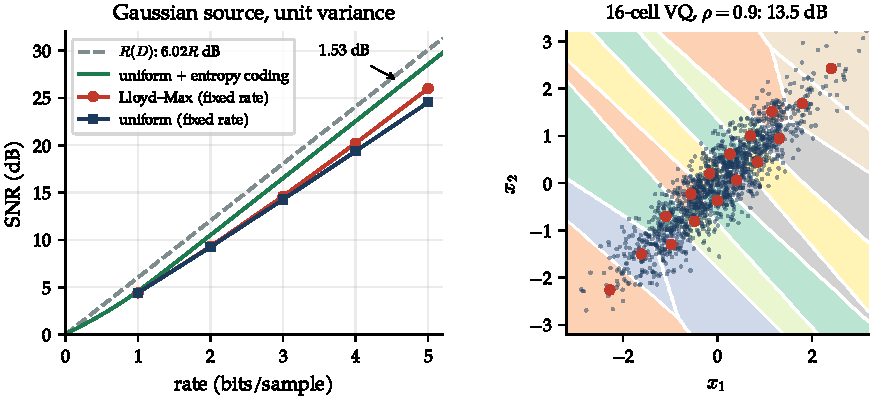
\includegraphics[width=0.92\linewidth]{figs/ch16_quantizers}\caption{Left: signal-to-noise ratio of quantisers for a unit-variance Gaussian
source. Fixed-rate quantisers (squares, circles) fall increasingly behind the rate--distortion
bound; a uniform quantiser followed by an ideal entropy coder (green) stays within 1.53\,dB
(0.254\,bit) of it at all rates above about one bit. Right: a 16-cell vector quantiser for pairs of
samples with correlation 0.9, designed with the Lloyd (k-means) algorithm on 20\,000 training
vectors. The cells follow the data, which a product of scalar quantisers cannot do; at the same
4 bits per pair the VQ achieves 13.5\,dB against 9.3\,dB for two independent 2-bit Lloyd--Max
quantisers.}\label{fig:ch16_quantizers}\end{figure}

\subsubsection{Entropy-coded scalar quantisation}

The surprise of the figure is the green curve. If the quantiser is allowed an \emph{unlimited}
number of uniformly spaced levels and its output is entropy coded, so that the rate is the entropy
of the quantiser index rather than the logarithm of the number of levels, the SNR at high rate is
\begin{equation}
\mathrm{SNR}_{\text{ECSQ}}\approx6.02\,R-1.53\ \mathrm{dB},
\label{eq:ch16:ecsq}
\end{equation}
within $10\log_{10}(\pi e/6)=1.53$\,dB, or $\tfrac12\log_2(\pi e/6)=0.254$ bits per sample, of the
rate--distortion bound. In plain words: the dumbest possible quantiser, evenly spaced rungs on a
ladder, is within a quarter of a bit of perfection, \emph{provided} an entropy coder makes the
common rungs cheap and the rare ones expensive.


\begin{deeper}[Where the 1.53\,dB comes from]
A uniform quantiser with small step $\Delta$ has distortion $\Delta^2/12$ and output entropy
$H\approx h(X)-\log_2\Delta$, where $h(X)$ is the differential entropy (each cell has probability
about $f(x)\Delta$). Eliminating $\Delta$ gives $D\approx\frac{1}{12}2^{2h(X)}2^{-2H}$, and for the
Gaussian $2^{2h(X)}=2\pi e\sigma^2$, so $D\approx\frac{\pi e}{6}\sigma^2 2^{-2H}$. Comparing with
$D(R)=\sigma^22^{-2R}$ gives the factor $\pi e/6=1.42$, or 1.53\,dB. The remarkable fact is that the
same 1.53\,dB gap to the Shannon lower bound holds for \emph{any} smooth source density, and that no
scalar quantiser of any shape, with or without entropy coding, does better at high rate. The
remaining 1.53\,dB is the \term{space-filling loss} of the cubic cell: in many dimensions, a cube
is a poor approximation to a sphere.
\end{deeper}

That result is the justification for the architecture of practically every modern codec: a
\emph{uniform} quantiser (with a slightly widened zero cell, the \term{deadzone}, which helps at low
rates) followed by a good adaptive entropy coder.

\subsection{Vector quantisation}


A \term{vector quantiser} (VQ) maps a block of $k$ samples to the nearest of $N$ code vectors,
sending $\log_2N$ bits, or $R=\log_2N/k$ bits per sample. Think of it as rounding not each number
separately but a whole list at once, to the nearest of a catalogue of typical lists. Shannon's
source coding theorem is itself a statement about vector quantisation in the limit $k\to\infty$,
and a VQ has three advantages over scalar quantisation, identified by Lookabaugh and Gray in 1989:
\begin{itemize}[nosep]
\item \emph{Space-filling advantage}: cells in $k$ dimensions can be more sphere-like than cubes (Figure~\ref{fig:ch16_vq_cells}).
This is what closes the 1.53\,dB gap, and only slowly: about 0.17\,dB for the hexagonal lattice in two
dimensions and about 1.0\,dB for the 24-dimensional Leech lattice.
\item \emph{Shape advantage}: cells can be concentrated where the probability density is high.
\item \emph{Memory advantage}: cells can follow the correlation between samples, as in the right
panel of Figure~\ref{fig:ch16_quantizers}, where the cells line up along the diagonal. For
correlated sources this is by far the largest gain.
\end{itemize}
\begin{figure}[H]\centering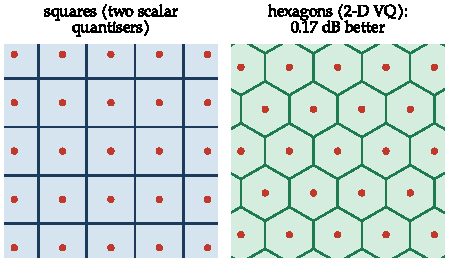
\includegraphics[width=0.5\linewidth]{figs/ch16_vq_cells}\caption{The space-filling advantage. Quantising two numbers separately tiles
the plane with squares; a two-dimensional vector quantiser can use hexagons, which are rounder and so
have a smaller mean-squared error for the same number of cells per unit area---0.17\,dB in two
dimensions, rising slowly towards 1.53\,dB as the dimension grows.}\label{fig:ch16_vq_cells}\end{figure}

Codebooks are designed with the generalised Lloyd algorithm (the LBG algorithm of Linde, Buzo and
Gray, 1980, known in machine learning as $k$-means): alternately assign training vectors to their
nearest code vectors and move each code vector to the centroid of its cell. The difficulty is
complexity: at $R$ bits per sample and dimension $k$ the codebook has $2^{kR}$ entries, so a
full-search VQ of 40-sample speech vectors at 1 bit per sample, with $2^{40}$ code vectors, is
impossible. Practical VQs are \emph{structured}: split and multistage VQ of LPC parameters in speech
codecs, the algebraic (sparse-pulse) codebooks of ACELP, the pyramid VQ of the CELT audio codec,
trellis-coded quantisation in JPEG~2000 Part~2, and, most recently, the residual VQ of neural audio
codecs (Section~\ref{sec:ch16:neural}). Most sources with memory, however, are handled a different
way: decorrelate first with a transform or a predictor, then use scalar quantisers.

\mdcfig{ch16_dct_recipe}{The DCT as a recipe. Top: a real $8\times8$ block from the portrait (chin
and lower lip) equals 222 units of the flat pattern, plus 208 of a vertical gradient, minus 207 of
a vertical cosine, and so on: five patterns carry almost all of it. Bottom: rebuilding the block
from the first 1, 3, 6, 10, 21 and 64 coefficients in zig-zag order. With ten coefficients the rms
error is under 8 grey levels.}

\begin{tryit}[Run Lloyd's algorithm by hand]
In Lab 24's \emph{Quantisers and Lloyd--Max} experiment, set \emph{Source distribution} to
Gaussian and \emph{Bits per sample} to 3, then drag \emph{Lloyd iterations} from 0 upwards one
step at a time. Watch the triangles (levels) slide outwards and the gain climb towards 0.35\,dB.
Switch to Laplacian---the peaky shape of speech samples and DCT coefficients---and the gain over a
uniform quantiser grows to well over a decibel. With Uniform, Lloyd has nothing to improve.
\end{tryit}

\subsection{Transform coding}

\begin{analogy}[A picture as a recipe of checkerboards]
You can describe an $8\times8$ patch of a photograph pixel by pixel---64 numbers, all about equally
important. Or you can describe it as a recipe: ``mostly this flat grey, plus a fair amount of a
dark-at-the-bottom gradient, plus a pinch of horizontal stripes'' (Figure~\ref{fig:ch16_dct_recipe}).
For natural images the recipe has a few big ingredients and many tiny ones, and you can leave the
tiny ones out without anyone tasting the difference. The discrete cosine transform finds that
recipe: it says how much of each of 64 standard checkerboard patterns the block contains. The
limit of the analogy: the patterns are fixed in advance, so content that is not smooth---text,
sharp edges, noise---needs many ingredients.
\end{analogy}

\mdcpairany{ch16_dct_basis}{The 64 basis images of the $8\times8$ two-dimensional DCT, from the
constant (DC) image at top left to the finest checkerboard at bottom right. Horizontal frequency
increases to the right, vertical frequency downwards. Every $8\times8$ block of a JPEG image is a
weighted sum of these patterns, and the weights are what the encoder quantises.}{ch16_compaction}{Energy
compaction on the portrait: averaged over all 1024 blocks, the first 6 DCT coefficients in zig-zag
order hold 93\% of the energy. For white noise of the same power (grey) every coefficient holds the
same share, and the transform buys nothing.}

Here is the mathematics behind the recipe. Consider a block of $N$ samples $\vect{x}$ with
covariance matrix $\vect{R}_x$ and an orthonormal transform $\vect{y}=\vect{T}\vect{x}$. The
coefficient $y_i$ has variance $\sigma_i^2$, and orthonormality preserves both total energy and
squared error, so quantisation noise in the coefficients appears unchanged in the reconstruction.
Suppose each coefficient is quantised with $b_i$ bits by a quantiser with distortion
$D_i=c\,\sigma_i^2\,2^{-2b_i}$ (the high-rate model; $c$ is 1 for an ideal coder and $\pi e/6$ for
ECSQ). Minimising $\sum_iD_i$ subject to an average rate $\bar b=\frac1N\sum_ib_i$ with a Lagrange
multiplier gives the classic \term{bit allocation} rule
\begin{equation}
b_i=\bar b+\frac12\log_2\frac{\sigma_i^2}{\left(\prod_j\sigma_j^2\right)^{1/N}},
\label{eq:ch16:bitalloc}
\end{equation}
with every coefficient getting the same distortion $D_i=c\,2^{-2\bar b}(\prod_j\sigma_j^2)^{1/N}$.
Read it as ``spend bits on big coefficients'': a coefficient with twice the standard deviation
gets one more bit. Compared with quantising the samples directly at $\bar b$ bits each, the
distortion falls by the \term{coding gain}
\begin{equation}
G_{\text{TC}}=\frac{\frac1N\sum_i\sigma_i^2}{\left(\prod_i\sigma_i^2\right)^{1/N}},
\label{eq:ch16:tcgain}
\end{equation}
the ratio of the arithmetic to the geometric mean of the coefficient variances. It is at least one,
with equality only when all variances are equal, and it is largest when the transform packs the
energy into as few coefficients as possible---exactly what Figure~\ref{fig:ch16_compaction} shows
for a real photograph.

The transform that maximises~\eqref{eq:ch16:tcgain} is the \term{Karhunen--Lo\`eve transform}
(KLT), whose rows are the eigenvectors of $\vect{R}_x$; the coefficients are then uncorrelated and
their variances are the eigenvalues. Since the product of the eigenvalues is $\det\vect{R}_x$, the
maximum gain is $(\operatorname{tr}\vect{R}_x/N)/(\det\vect{R}_x)^{1/N}$. As $N\to\infty$ this
approaches the reciprocal of the \term{spectral flatness measure} of the source, the ratio of the
geometric to the arithmetic mean of its power spectral density---exactly the same limit as the gain
of an optimum infinite-order predictor. Transform coding and predictive coding are two routes to the
same destination.

\subsubsection{Why the DCT}

The KLT depends on the signal statistics, must be computed and transmitted, and has no fast
algorithm. For the first-order autoregressive (AR(1)) model, $R_x[k]=\sigma^2\rho^{|k|}$, which is a
reasonable model of image rows and columns with $\rho$ around 0.9--0.95, the eigenvectors of
$\vect{R}_x$ approach the basis functions of the \term{discrete cosine transform} as $\rho\to1$. The
DCT-II,
\begin{equation}
y_k=\alpha_k\sum_{n=0}^{N-1}x_n\cos\frac{\pi(2n+1)k}{2N},\qquad
\alpha_0=\sqrt{1/N},\ \alpha_{k>0}=\sqrt{2/N},
\label{eq:ch16:dct}
\end{equation}
was introduced by Nasir Ahmed, T.~Natarajan and K.~R.~Rao in 1974 precisely because its
performance was close to the KLT's for such sources while it had a fast, signal-independent
algorithm. Figure~\ref{fig:ch16_coding_gain} (left) shows how close: for $\rho=0.95$ and $N=8$
the KLT gain is 8.85\,dB and the DCT's is 8.83\,dB. The DCT also avoids the artificial
discontinuity that the discrete Fourier transform creates at the block edges, because it
implicitly extends the block symmetrically rather than periodically. The eight-point DCT has
become one of the most computed transforms in history: it is inside every JPEG, MPEG and H.26x
codec, and the integer transforms of H.264, HEVC and VVC are its descendants.

\begin{worked}[The coding gain of a two-point transform]
Take pairs of samples from an AR(1) source with unit variance and correlation $\rho=0.95$. The
covariance matrix is $\begin{bsmallmatrix}1&\rho\\ \rho&1\end{bsmallmatrix}$, whose eigenvectors are
$(1,1)/\sqrt2$ and $(1,-1)/\sqrt2$---the two-point DCT, sum and difference---with eigenvalues
$1+\rho=1.95$ and $1-\rho=0.05$. The coding gain~\eqref{eq:ch16:tcgain} is
\[
G=\frac{(1.95+0.05)/2}{\sqrt{1.95\times0.05}}=\frac{1}{\sqrt{1-\rho^2}}=\frac{1}{\sqrt{0.0975}}=3.20,
\]
or 5.05\,dB, worth 0.84 bits per sample. By~\eqref{eq:ch16:bitalloc}, at an average of 2 bits per
sample the sum coefficient gets $2+\frac12\log_2(1.95/0.312)=3.32$ bits and the difference
coefficient $0.68$ bits (the geometric mean of the variances is $\sqrt{0.0975}=0.312$); the 4 bits
per pair are shared unequally because the energy is. With $N=8$ the gain rises to 8.83\,dB
(Figure~\ref{fig:ch16_coding_gain}), and the limit for $N\to\infty$ is $1/(1-\rho^2)=10.26$, or
10.1\,dB. Most of the available gain is captured by blocks of eight, which is one reason the early
standards chose $8\times8$: bigger blocks gained little and cost more memory and multiplications, and
on real images, which are not stationary, larger blocks also spread quantisation errors over a
larger area.
\end{worked}

\mdcfig{ch16_coding_gain}{Left: coding gain of the KLT (solid, pale) and the DCT (dashed) for an
AR(1) source, for block sizes 4, 8 and 16; the dotted curve is the infinite-block limit
$1/(1-\rho^2)$. The DCT is within a few hundredths of a decibel of the optimum. Right: variances of
the 64 coefficients of the $8\times8$ DCT measured on the 256$\times$256 portrait of
Figure~\ref{fig:ch16_jpeg_quality}, sorted, with the reverse water-filling level for an average of
1 bit per pixel. Only 47 coefficients rise above the water level and receive bits (orange curve);
the DC coefficient receives almost 6.}

\begin{tryit}[Throw away coefficients]
In Lab 24, open \emph{DCT energy compaction} with the \emph{Photograph}. Move \emph{Block column}
and \emph{Block row} onto a smooth cheek, then onto an eye, and drag \emph{Coefficients kept}
from 64 down to 3. On the smooth block three coefficients look perfect; on the eye they do not.
Then switch \emph{Image} to \emph{White noise}: the coefficient bars flatten out and no amount of
cleverness lets you drop any.
\end{tryit}

\subsubsection{Reverse water-filling}

The bit allocation~\eqref{eq:ch16:bitalloc} can produce negative $b_i$ for coefficients with small
variance, which is meaningless. The exact solution for Gaussian coefficients, from rate--distortion
theory, is \term{reverse water-filling}. Picture the coefficient variances as a row of hills of
different heights, and flood the landscape to a ``water level'' $\theta$. Each coefficient gets
\begin{equation}
D_i=\min(\theta,\sigma_i^2),\qquad R_i=\max\!\Big(0,\tfrac12\log_2\frac{\sigma_i^2}{\theta}\Big),
\label{eq:ch16:reversewf}
\end{equation}
and $\theta$ is adjusted until the total rate matches the budget. Only the hilltops that stick out
of the water are described; the submerged ones are not sent at all, and the decoder sets them to
zero and accepts their whole variance as distortion. This is the theoretical basis of the most
visible behaviour of every transform codec: at low rates, high-frequency coefficients are discarded
entirely. On the real image of Figure~\ref{fig:ch16_coding_gain}, the 64 DCT coefficients have a
coding gain of 12.6\,dB, and at an average of 1 bit per pixel reverse water-filling gives bits to
47 of them and nothing to the other 17.

Practical codecs use quantisation tables and deadzones rather than explicit bit allocation because,
with entropy coding, a uniform quantiser with the same step size for every coefficient implements
\eqref{eq:ch16:reversewf} automatically: equal steps mean equal distortion, the entropy coder spends
about $\frac12\log_2(\sigma_i^2/\theta)$ bits where the variance is large, and a coefficient smaller
than half a step quantises to zero and costs almost nothing.


\begin{figure}[H]\centering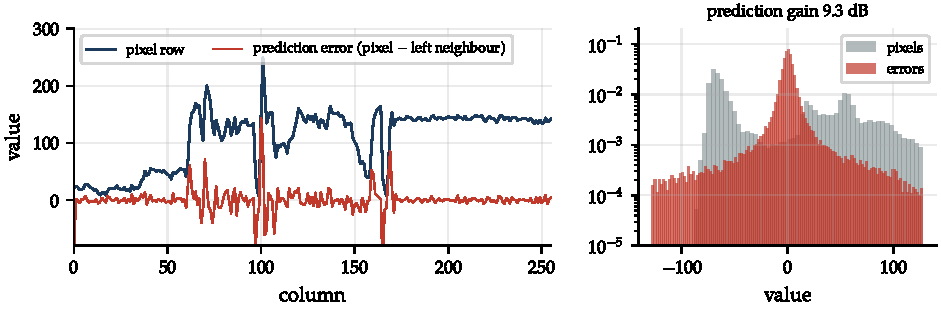
\includegraphics[width=0.92\linewidth]{figs/ch16_dpcm_residual}\caption{Prediction at work on the portrait. Left: one row of pixels (navy)
and the error of the simplest possible predictor, ``same as the pixel to the left'' (red), which is
near zero except at edges. Right: over the whole image the errors are sharply peaked at zero, and
their variance is 9.3\,dB below that of the pixels---a prediction gain worth about 1.5 bits per
pixel.}\label{fig:ch16_dpcm_residual}\end{figure}

\subsection{Predictive coding and the spectral flatness}

The differential PCM of Chapter~\ref{ch:pcm} is the other route to decorrelation: instead of
describing each sample, describe how wrong your best guess was. A linear predictor of order $p$
estimates $x_n$ from $x_{n-1},\dots,x_{n-p}$, and only the prediction error (Figure~\ref{fig:ch16_dpcm_residual}), with variance
$\sigma_e^2$, is quantised. The \term{prediction gain} $G_p=\sigma_x^2/\sigma_e^2$ increases with
order to the limit
\begin{equation}
G_\infty=\frac{\frac{1}{2\pi}\int_{-\pi}^{\pi}S_x(e^{j\omega})\,d\omega}{\exp\!\left(\frac{1}{2\pi}\int_{-\pi}^{\pi}\ln S_x(e^{j\omega})\,d\omega\right)}
=\frac{1}{\gamma_x^2},
\label{eq:ch16:sfm}
\end{equation}
where $\gamma_x^2$ is the spectral flatness measure: one for white noise, near zero for a sharply
peaked spectrum. In words: the more ``coloured'' the spectrum, the more predictable the signal and
the bigger the gain. It is the same quantity that limits the coding gain of an infinitely large
transform, and for an AR(1) source $G_\infty=1/(1-\rho^2)$, already reached with a first-order
predictor.

The two approaches differ in the details: prediction works sample by sample with no block delay and
suits low-delay speech coding, while transform coding lets the quantisation noise be shaped in
frequency, which perceptual coding needs. The predictor must run on reconstructed samples (closed
loop), or quantisation errors accumulate at the decoder---a lesson re-learned by every generation of
video coding engineers, who call the resulting divergence \term{drift}.

\begin{keyidea}[Decorrelate, quantise uniformly, entropy code]
For sources with memory, the best practical recipe is to decorrelate the samples with a transform
or a predictor, quantise the resulting values with uniform (deadzone) scalar quantisers of equal
step size, and entropy code the indices with an adaptive context model. The transform supplies the
memory advantage, the equal steps implement reverse water-filling, and the entropy coder recovers
most of the shape advantage, leaving the 1.53\,dB space-filling loss as the main price of
simplicity. Perceptual codecs modify only one thing: they make the step size depend on how audible
or visible the error is in each coefficient.
\end{keyidea}

\mdcfig{ch16_mse_perception}{Same error power, very different pictures. Each image has a PSNR of
about 23.7\,dB against the original: brightened by a constant (barely noticeable), blurred (clearly
soft), and JPEG-coded at quality 5 (blocky). A mean-squared-error meter cannot tell them apart; your
eye ranks them instantly.}

\begin{pitfall}[Mean-squared error is not what people perceive]
All the theory above minimises mean-squared error because it is tractable, not because it is right.
A codec tuned only for SNR or PSNR produces blurry images and muffled speech that score well
numerically and look or sound worse than a codec that preserves texture and sharpness at a lower
PSNR. Speech codecs weight their error spectrally; audio codecs follow a masking model; image and
video codecs are increasingly tuned with perceptual metrics (SSIM, VMAF and learned metrics) and
with ``psycho-visual'' options that deliberately put energy back into flattened textures. Always
check a codec's output by looking and listening, and be suspicious of any comparison made at a
single PSNR value. Figure~\ref{fig:ch16_mse_perception} makes the point with three pictures of
identical PSNR.
\end{pitfall}

%======================================================================
\section{Speech coding}
\label{sec:ch16:speech}
%======================================================================

Why does a phone call sound like a phone call? Close your eyes while a friend talks to you across
a table and then over an old landline, and you would never confuse the two. The landline voice is
thin and a little muffled; ``f'' and ``s'' blur together, which is why people spell names on the
phone with ``S as in Sugar''. The reason is not the codec at all but the band: the classic
telephone channel passes only 300--3400\,Hz, and Figure~\ref{fig:ch16_phone_band} shows what that
does to a hissing /s/. The handset itself (Figure~\ref{fig:ch16_handset}) was built for that band. Today's ``HD voice'' codecs widen the band to 7\,kHz or more, and the
difference is immediately audible.


\mdcpairany[H]{ch16_handset}{Inside a telephone handset: a dynamic microphone capsule at one end and
an earpiece at the other. For a century the network behind it was engineered around the
300--3400\,Hz band that these transducers and the loaded cable pairs could carry.}{ch16_phone_band}{Why
a phone call sounds ``phone-y''. A vowel's energy sits mostly below 3.4\,kHz, but almost all of the
energy of a fricative /s/ lies above it: in this synthetic example only 1.6\% of it survives the
telephone band (navy), while a 7\,kHz wideband (``HD voice'') channel keeps 84\% of it (green).}

Speech was the first signal to be compressed and remains the one for which the most specialised
models exist, because it comes from a single, well-understood instrument. Its codecs span a range
of rates from below 1\,kb/s to 64\,kb/s, and the story of how the rate fell by a factor of eight
without losing quality is the story of linear prediction.

\subsection{How speech is produced}

\mdcpairany{ch16_vocaltract}{The instrument: a mid-sagittal section of the head. The vocal tract
runs from the vocal folds (black, in the larynx) up through the pharynx and out through the mouth,
with the nasal cavity as a side branch. Its length, about 17\,cm in an adult man, sets the formant
frequencies.}{ch16_vocalfolds}{The vocal folds seen from above through a laryngoscope, held open for
breathing. In voiced speech they snap together and apart about a hundred times a second, chopping
the airflow into the pulses of the ``buzz''.}

\begin{analogy}[A buzz shaped by a tube]
Blow a raspberry through your lips and you have a buzz; hum through a cardboard tube and the tube
colours the buzz. Your voice works the same way. The vocal folds in your larynx chop the airflow
from your lungs into a buzz of pulses---about 120 a second for a typical man's voice. The throat
and mouth form a tube about 17\,cm long whose shape, set by your tongue, jaw and lips, makes
some frequencies ring and others die away (Figure~\ref{fig:ch16_source_filter}). Change the tube's
shape and the same buzz becomes ``ah'', ``ee'' or ``oo''. The limit of the analogy: for consonants
like /s/ and /f/ there is no buzz at all, just the hiss of air forced through a narrow gap.
\end{analogy}

Air from the lungs passes through the larynx, where the vocal folds either vibrate or stay open,
and then through the \emph{vocal tract}---the pharynx, mouth and, for nasal sounds, the nasal
cavity---before radiating from the lips (Figures~\ref{fig:ch16_vocaltract} and~\ref{fig:ch16_vocalfolds}). Two kinds of excitation
result. In \emph{voiced} sounds (vowels, and consonants such as \emph{m}, \emph{l} and \emph{z})
the folds open and close periodically, producing a train of airflow pulses at the
\term{fundamental frequency} or \emph{pitch} $f_0$, typically 80--180\,Hz for adult men,
160--300\,Hz for women and higher for children. In \emph{unvoiced} sounds (\emph{s}, \emph{f},
\emph{sh}) the excitation is turbulent noise generated at a constriction. Plosives (\emph{p},
\emph{t}, \emph{k}) add a brief burst after a closure.

The vocal tract shapes the excitation's spectrum. Its resonances, the \term{formants}, appear as
peaks in the spectral envelope at roughly 500, 1500 and 2500\,Hz for a uniform tube, and the
tongue, jaw and lips move them to make the different vowels: /a/ as in \emph{father} has its
first two formants near 730 and 1090\,Hz, /i/ as in \emph{beet} near 270 and 2290\,Hz
(Figures~\ref{fig:ch16_vowel_chart} and~\ref{fig:ch16_spectrogram}). This is the \term{source--filter model}: speech is an
excitation (periodic pulses or noise) passed through a slowly varying linear filter.

\mdcfig{ch16_source_filter}{The source--filter model in three pictures. Left: the glottal buzz is a
comb of harmonics at multiples of the pitch (here 125\,Hz), falling smoothly with frequency. Centre:
the vocal tract for /a/ is a filter with resonances---formants---near 730, 1090, 2440 and
3400\,Hz. Right: the vowel's spectrum is their product: the same harmonics, now with the formant
envelope (pale) stamped on them.}

The filter changes as the articulators move, but slowly---over tens of milliseconds---so it can be
treated as fixed over a \emph{frame} of 10--30\,ms. The consequence for compression is profound.
Instead of coding the waveform, a codec can send the filter parameters and a description of the
excitation once per frame. A 20\,ms frame of 8\,kHz speech has 160 samples, but the filter is
described by about ten numbers.

Figure~\ref{fig:ch16_vowel_lpc} shows the model at work on a synthetic vowel /a/, generated by
passing a train of glottal pulses at 120\,Hz through four formant resonators and a lip-radiation
differentiator---a classic formant synthesiser in the tradition of Dennis Klatt's. The spectrum
(panel b) shows the fine structure of the pitch harmonics, 120\,Hz apart, under the smooth envelope
of the formants.

\mdcpairany{ch16_vowel_chart}{The vowel map: average first and second formant frequencies of
American English vowels spoken by men, from the classic 1952 measurements of Peterson and Barney.
Axes are reversed so that the chart resembles the position of the tongue in the
mouth.}{ch16_spectrogram}{A spectrogram of synthetic speech: /a/, /s/, /i/, /u/. Horizontal
stripes are the pitch harmonics; the dark bands that move from vowel to vowel are the formants. The
/s/ is a cloud of noise above 4\,kHz, almost entirely above the telephone cut-off
(dashed).}

\subsection{Linear prediction}
\label{sec:ch16:lpc}

\mdcfig{ch16_vowel_lpc}{Linear prediction of a synthetic vowel /a/ (8\,kHz sampling). (a) The
speech waveform and the prediction residual $e[n]$ of a 10th-order LPC inverse filter: the
residual is nearly white apart from sharp pulses at the glottal closures, 8.3\,ms apart.
(b) The periodogram of a 32\,ms Hamming-windowed frame and the LPC envelope $E_p/|A(e^{j\omega})|^2$,
which captures the formants (dotted lines at their true frequencies) and ignores the harmonics.
(c) Prediction gain against predictor order: two coefficients capture most of the spectral tilt,
ten capture the formants, and higher orders add almost nothing. (d) The poles of $1/A(z)$ and the
roots of the line-spectral polynomials $P(z)$ and $Q(z)$, which lie on the unit circle and
interleave; pairs of LSFs cluster around each formant.}

How do we measure the tube from the sound alone? The trick is prediction. If the tube rings,
each sample is largely an echo of the last few, so we can guess it from them; the part we
\emph{cannot} guess is the buzz. Fitting the best predictor is therefore the same as measuring the
tube, and what the predictor misses is the excitation.

\term{Linear predictive coding} (LPC) fits an all-pole filter $1/A(z)$ to each frame, with
\begin{equation}
A(z)=1+\sum_{k=1}^{p}a_kz^{-k},\qquad e[n]=s[n]+\sum_{k=1}^pa_k\,s[n-k],
\label{eq:ch16:lpc}
\end{equation}
by minimising the energy of the prediction error $e[n]$. An all-pole model fits the source--filter
picture well: a lossless acoustic tube made of $p$ sections of equal length has exactly an all-pole
transfer function, and each formant corresponds to a pair of complex poles. Setting the derivative
of $\sum_ne^2[n]$ with respect to each $a_k$ to zero gives the \term{normal equations}
\begin{equation}
\sum_{k=1}^pa_k\,r[|i-k|]=-r[i],\qquad i=1,\dots,p,
\label{eq:ch16:normal}
\end{equation}
where, in the \emph{autocorrelation method}, $r[m]=\sum_n s_w[n]s_w[n+m]$ is computed from the
frame multiplied by a tapered window (Hamming, or an asymmetric window in low-delay codecs). The
matrix is symmetric Toeplitz and positive definite, which guarantees two things: the equations can
be solved in $O(p^2)$ operations, and the resulting synthesis filter $1/A(z)$ is always stable. (The
alternative \emph{covariance method} computes the correlation without windowing; it fits short frames
better but does not guarantee stability.)

\begin{deeper}[The Levinson--Durbin recursion]
The recursion that solves~\eqref{eq:ch16:normal}, found by Norman Levinson in 1947 for Wiener
filtering and refined by James Durbin in 1960, builds the order-$i$ predictor from the order-$(i-1)$
one. Start with $E_0=r[0]$ and for $i=1,\dots,p$ compute
\begin{align}
k_i&=-\frac{r[i]+\sum_{j=1}^{i-1}a_j^{(i-1)}\,r[i-j]}{E_{i-1}},\label{eq:ch16:levk}\\
a_i^{(i)}&=k_i,\qquad a_j^{(i)}=a_j^{(i-1)}+k_i\,a_{i-j}^{(i-1)}\quad(j=1,\dots,i-1),\\
E_i&=(1-k_i^2)\,E_{i-1}.\label{eq:ch16:leve}
\end{align}
The numbers $k_i$ are the \term{reflection coefficients} (or PARCOR, partial correlation,
coefficients, the name used by Fumitada Itakura and Shuzo Saito, who developed LPC for speech in
Japan in the late 1960s at the same time as Bishnu Atal and Manfred Schroeder at Bell Labs). They
have a physical meaning: in the acoustic-tube model, $k_i$ is the fraction of the pressure wave
reflected at the junction between tube sections $i$ and $i+1$, determined by the ratio of their
cross-sectional areas. Equation~\eqref{eq:ch16:leve} shows that the error energy falls at every step
and that stability is equivalent to $|k_i|<1$ for all $i$, a condition trivially checked after
quantisation. The reflection coefficients also define the \emph{lattice filter} structure, which
implements $A(z)$ or $1/A(z)$ stage by stage and is robust to coefficient quantisation.
\end{deeper}

\mdcfig{ch16_lpc_orders}{What the predictor order buys, on a frame of the synthetic vowel /a/.
Order 1 captures only the spectral tilt; orders 2 and 4 find one broad hump; order 10 resolves all
four formants at 730, 1090, 2440 and 3400\,Hz and ignores the harmonic fine structure, which is left
for the excitation to describe.}

\begin{worked}[A second-order predictor by hand]
A voiced frame has normalised autocorrelation $r[0]=1$, $r[1]=0.8$, $r[2]=0.5$. Find the
second-order LPC filter, its prediction gain and its resonance.

Step 1: $k_1=-r[1]/r[0]=-0.8$, so $a_1^{(1)}=-0.8$ and $E_1=(1-0.64)=0.36$. A first-order predictor
removes 64\% of the energy, a gain of $1/0.36=2.78$ (4.4\,dB).

Step 2: $k_2=-(r[2]+a_1^{(1)}r[1])/E_1=-(0.5-0.64)/0.36=0.389$. Then $a_2=0.389$,
$a_1=-0.8+0.389\times(-0.8)=-1.111$ and $E_2=0.36(1-0.389^2)=0.306$, a gain of 3.27 (5.1\,dB). The
filter is $A(z)=1-1.111z^{-1}+0.389z^{-2}$; you can check that the predictor coefficients
$(1.111,-0.389)$ satisfy~\eqref{eq:ch16:normal}.

The roots of $z^2-1.111z+0.389$ are $0.556\pm j0.283$, with radius $\sqrt{0.389}=0.624$ and angle
$27.0^\circ$. At 8\,kHz sampling the angle corresponds to $27.0/360\times8000=600$\,Hz, and the radius
to a 3\,dB bandwidth of roughly $-f_s\ln(0.624)/\pi=1.2$\,kHz: a single broad resonance, which is all
two coefficients can describe (Figure~\ref{fig:ch16_lpc_orders}). With order 10, as in panel (d) of Figure~\ref{fig:ch16_vowel_lpc},
the poles of the synthetic /a/ land at 706, 1089, 2443 and 3402\,Hz with radii 0.94--0.97, tracking the
true formants to within a few per cent.
\end{worked}

\subsubsection{Line spectral frequencies}

The filter coefficients $a_k$ are poor parameters for quantisation and transmission: small errors
can move poles outside the unit circle, and the coefficients cannot be interpolated between frames.
Reflection coefficients are better (stability is easy to check), but the representation used by
virtually every modern speech codec is the set of \term{line spectral frequencies} (LSFs), or line
spectral pairs, introduced by Itakura in 1975. Form the two polynomials
\begin{equation}
P(z)=A(z)+z^{-(p+1)}A(z^{-1}),\qquad Q(z)=A(z)-z^{-(p+1)}A(z^{-1}),
\label{eq:ch16:lsf}
\end{equation}
the transfer functions of the acoustic tube with the glottis end fully closed and fully open.
Their roots lie \emph{on} the unit circle, and if $A(z)$ is minimum phase they \emph{interleave}:
$0<\omega_1<\omega_2<\dots<\omega_p<\pi$, alternating between $P$ and $Q$ (panel d of
Figure~\ref{fig:ch16_vowel_lpc}). The $p$ angles are the LSFs. They behave like frequencies: they
cluster in pairs around each formant (in the figure, 1055 and 1162\,Hz bracket the second formant),
they vary smoothly from frame to frame and can be interpolated, the ordering property gives an
immediate stability check, and an error in one LSF affects the spectrum only near that frequency.
Split or multistage vector quantisers code ten LSFs in 18--46 bits per frame with an average spectral
distortion of about 1\,dB, the accepted threshold of transparency.

\begin{tryit}[Be a vocoder]
Lab 24's \emph{LPC: a buzz and a filter} analyses a synthetic vowel and resynthesises it. Pick
\emph{Vowel} /a/ and press both \emph{Listen} buttons. Now drag \emph{LPC order p} down to 2 and
listen again: the vowel turns into a dull ``uh'' because two coefficients describe one broad
resonance. Restore $p=10$, then drag \emph{New pitch} from 180 to 300\,Hz---the same tube, a
different buzz---and finally set \emph{Resynthesis excitation} to \emph{Noise (whisper)}.
\end{tryit}

\subsection{Vocoders: sending the model, not the wave}

A \term{vocoder} (voice coder) transmits only the model: the filter parameters, a voiced/unvoiced
decision, the pitch and the gain. The decoder regenerates the excitation from a pulse train or a noise
generator and passes it through the synthesis filter. Because no attempt is made to match the
waveform, the rate can be extremely low, and the speech, though intelligible, sounds synthetic---the
famous buzzy ``robot'' quality of military radio.


\mdcphoto[0.45]{ch16_stu3}{A STU-III secure telephone (introduced 1987), on display at the US
National Cryptologic Museum. Its 2.4\,kb/s LPC-10 mode let encrypted speech cross an ordinary
telephone line through a modem.}

The US Federal Standard 1015 \term{LPC-10} vocoder (1984) sends ten reflection coefficients, pitch,
voicing and gain in 54 bits every 22.5\,ms, a total of 2.4\,kb/s, which fitted the HF radio and secure
telephone (STU-III, Figure~\ref{fig:ch16_stu3}) channels of its day. Its successor, the \term{MELP} (mixed-excitation linear
prediction) coder, selected as the new US federal standard in 1996 (later MIL-STD-3005), mixes pulse
and noise excitation in several frequency bands, adds aperiodic pulses for transitions and shapes the
pulses, and gives much more natural speech at the same 2.4\,kb/s. Its enhanced version MELPe is
NATO's standard STANAG 4591 at 2.4, 1.2 and 0.6\,kb/s.

Vocoders live on wherever bits are extremely scarce: in military tactical radio, in satellite
telephony (the IMBE and AMBE family of multiband-excitation vocoders in Iridium, Inmarsat and
digital land-mobile radio such as P25 and DMR, at 2.4--4.8\,kb/s), and in open-source amateur-radio
codecs such as Codec~2 at 0.7--3.2\,kb/s. What they all share is the bet that the listener needs to
understand the words, not to hear the exact waveform. At 2.4\,kb/s, a vocoder sends roughly one bit
for every three samples of telephone speech; even the earliest digital telephone channel spent
eight. The cost is naturalness, and the remarkable achievement of the next twenty years of speech
coding was to buy most of the naturalness back while staying far closer to the vocoder's rate
than to PCM's.

\mdcpairany{ch16_voder}{The Voder at the 1939 New York World's Fair, at the Bell System exhibit. An
operator at the console ``played'' speech with keys selecting band-pass filters, a wrist bar
switching between buzz and hiss, and a foot pedal setting the pitch---a source--filter synthesiser
built from vacuum tubes. Photograph from Dudley's 1940 \emph{Bell System Technical Journal}
paper.}{ch16_sigsaly_record}{A SIGSALY key record at the US National Cryptologic Museum. Each
phonograph disc carried random key values that were added, modulo six, to the quantised vocoder
channels; only two copies of each record were made, one for each end of the link, and each was used
once.}

\begin{history}[From the Voder to SIGSALY]
Homer Dudley of Bell Telephone Laboratories began working on the vocoder in the late 1920s,
motivated by the enormous cost of transatlantic telephone bandwidth. His insight was that the
information in speech lies in the slow movements of the articulators, which change a few tens of
times per second, not in the kilohertz waveform. His vocoder, patented in the 1930s, analysed speech
with a bank of ten band-pass filters, sent the slowly varying energy in each band together with a
pitch signal, and resynthesised the speech from a buzz or hiss source at the far end. Its manual
cousin, the \emph{Voder}, was operated by trained women at a keyboard and pedal board and ``spoke''
to amazed crowds at the 1939 New York World's Fair (Figure~\ref{fig:ch16_voder}).

The vocoder's first serious use was secret. In 1943 Bell Labs and the US Army put into service
SIGSALY, a secure telephone system linking Washington and London (and later other Allied
headquarters). A vocoder reduced speech to about a dozen slowly varying channels (ten spectral bands
plus pitch information), each sampled 50 times a second and quantised to six levels; each sample was
then added, modulo six, to a random key sample from a phonograph record (Figure~\ref{fig:ch16_sigsaly_record}) of which exactly two copies
existed, one at each end---a one-time pad applied to digitised speech. Each terminal filled a room,
weighed tens of tonnes and needed its own air conditioning. Allied leaders, Churchill among them, and
their senior commanders used it for the rest of the war, and it was never broken. SIGSALY was one of
the first practical systems to transmit speech in digital form, and Alan Turing, who visited Bell
Labs in 1943, studied it before designing his own speech scrambler. The line from SIGSALY runs
through LPC-10 and MELP to the vocoder in every modern military radio.
\end{history}

\begin{figure}[htbp]\centering
\begin{tikzpicture}[
  blk/.style={draw=navy,fill=navy!6,thick,minimum height=0.85cm,minimum width=1.6cm,align=center,font=\sffamily\scriptsize},
  arr/.style={-{Stealth[length=2mm]},thick,navy},
  sm/.style={draw=accent,circle,thick,minimum size=0.5cm,inner sep=0pt,font=\sffamily\small}]
\node[blk] (acb) at (0,1.1) {Adaptive codebook\\(past excitation,\\pitch lag $T$)};
\node[blk] (fcb) at (0,-0.6) {Fixed (algebraic)\\codebook,\\index $c$};
\node[sm] (ga) at (2.1,1.1) {$\times$};
\node[sm] (gc) at (2.1,-0.6) {$\times$};
\node[sm] (sum) at (3.2,0.25) {$+$};
\node[blk] (syn) at (4.9,0.25) {LPC synthesis\\$1/\hat A(z)$};
\node[sm] (err) at (6.6,0.25) {$-$};
\node[blk] (w) at (8.4,0.25) {Perceptual\\weighting\\$W(z)$};
\node[blk,fill=accent!8,draw=accent] (min) at (8.4,-1.45) {Minimise\\weighted\\error energy};
\node[blk,fill=green!6,draw=green!50!black] (lpc) at (4.9,1.85) {LPC analysis,\\LSF quantisation};
\node[font=\sffamily\scriptsize] (in) at (6.6,2.7) {input speech $s[n]$};
\draw[arr] (acb)--(ga); \draw[arr] (fcb)--(gc);
\draw[arr] (ga)--(sum); \draw[arr] (gc)--(sum);
\draw[arr] (sum)--node[above,font=\scriptsize]{$u[n]$}(syn); \draw[arr] (syn)--node[below,font=\scriptsize]{$\hat s[n]$}(err);
\draw[arr] (in)--(err); \draw[arr] (in.west) -| (lpc.north); \draw[arr,green!50!black] (lpc)--(syn);
\draw[arr] (err)--(w); \draw[arr] (w)--(min);
\node[font=\scriptsize,above=1pt of ga] {$g_p$}; \node[font=\scriptsize,above left=0pt and 0pt of gc] {$g_c$};
\draw[arr,accent,dashed] (min.west) -- (2.1,-1.45) -- (gc.south);
\draw[arr,accent,dashed] (2.1,-1.45) -- (-1.3,-1.45) |- (acb.west);
\node[font=\sffamily\scriptsize,text=accent] at (4.9,-1.7) {choose $T$, $c$, $g_p$, $g_c$};
\draw[arr,navy!60,dashed] (sum.north) |- (0,2.55) -- (acb.north);
\node[font=\sffamily\tiny,text=navy!70,anchor=south] at (1.6,2.55) {past excitation fed back};
\end{tikzpicture}
\caption{The CELP encoder. The excitation $u[n]$ is the sum of a scaled segment of the past
excitation (the adaptive codebook, which models the pitch periodicity) and a scaled sparse vector
from a fixed codebook. The encoder synthesises each candidate through the quantised LPC filter,
compares it with the input through a perceptual weighting filter and transmits the indices and gains
that minimise the weighted error. The decoder is the upper-left half of the diagram.}
\label{fig:ch16_celp}
\end{figure}

\subsection{Waveform coders: PCM and ADPCM}

At the other extreme, \emph{waveform coders} try to reproduce the waveform sample by sample and
make no assumption about the signal, so they work for any audio in the band---music, modem tones,
DTMF signalling---and degrade gracefully. G.711 PCM at 64\,kb/s is the reference
(Chapter~\ref{ch:pcm}). \term{ADPCM} (adaptive differential PCM) in ITU-T G.726 (1990, merging the
earlier G.721 and G.723) runs at 16, 24, 32 or 40\,kb/s. It uses a backward-adaptive pole--zero
predictor (two poles, six zeros) and a backward-adaptive quantiser step (Figure~\ref{fig:ch16_adpcm}), both computed from the
past decoded signal so that no side information is sent. At 32\,kb/s it gives quality close to G.711
and it is the codec of DECT cordless telephones. ITU-T G.722 (1988) splits wideband speech into two
subbands with a quadrature-mirror filterbank and codes each with ADPCM at 48--64\,kb/s total; it was
the first wideband telephony codec and is still common in DECT and IP phones.


\begin{figure}[H]\centering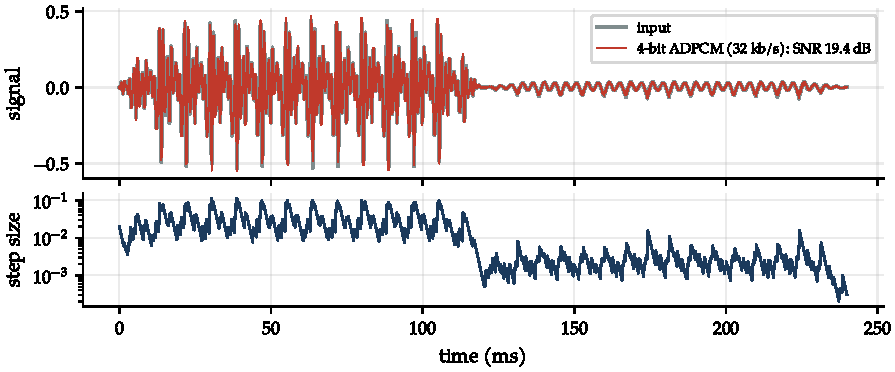
\includegraphics[width=0.92\linewidth]{figs/ch16_adpcm}\caption{Backward adaptation at work in a toy 4-bit ADPCM coder (a fixed first-order
predictor and a Jayant step-size rule, simpler than G.726). When the loud vowel gives way to a quiet
one, the step size (bottom) shrinks about tenfold within a few milliseconds, learned from the decoded
signal alone, so no side information is sent and the quiet vowel is coded as accurately as the loud
one. Overall SNR: 19.4\,dB at 32\,kb/s.}\label{fig:ch16_adpcm}\end{figure}

\subsection{Analysis by synthesis: CELP}

Waveform coders are robust but need 16\,kb/s or more; vocoders are efficient but sound synthetic.
\term{Code-excited linear prediction} (\term{CELP}), published by Manfred Schroeder and Bishnu Atal in
1985, found the middle ground that has dominated speech coding ever since. It keeps the LPC
synthesis filter of the vocoder but replaces the crude pulse-or-noise excitation with one chosen
from a codebook \emph{by trying the candidates and listening to the result}: the encoder contains a
copy of the decoder and selects the excitation whose synthesised output best matches the input,
according to a perceptually weighted error. Think of a tailor who, instead of measuring you, holds
up every jacket in the shop and picks the one that looks best in the mirror. This
\term{analysis-by-synthesis} principle (Figure~\ref{fig:ch16_celp}) makes the codec a waveform coder
of the vocal-tract output while sending only a vocoder's worth of parameters.


A CELP encoder processes each frame (typically 20\,ms) in four steps.
\begin{enumerate}[nosep]
\item \textbf{Short-term prediction.} Compute a 10th-order LPC filter from a windowed segment,
convert to LSFs, vector quantise them and interpolate between frames for each 5\,ms
\emph{subframe}.
\item \textbf{Long-term (pitch) prediction.} Voiced excitation is nearly periodic. The
\term{adaptive codebook} holds the excitation of the recent past; a candidate is the past excitation
delayed by a lag $T$ (in fractional samples, with $1/3$- or $1/4$-sample resolution) and scaled by a
gain $g_p$. The encoder searches the lag, first open-loop on the weighted speech once per frame and
then closed-loop around that estimate in each subframe.
\item \textbf{Innovation.} What the pitch predictor cannot explain is modelled by a vector from the
\term{fixed codebook}, scaled by $g_c$. Early CELP used random Gaussian codebooks, whose search cost a
supercomputer's attention (the first CELP simulations reportedly needed more than a minute of
Cray-1 time per second of speech). Modern codecs use \term{algebraic codebooks} (ACELP): each code vector
contains only a few pulses of amplitude $\pm1$ at positions restricted to interleaved tracks, so it
needs no storage and can be searched quickly with nested loops and pruning.
\item \textbf{Gains.} The two gains are vector quantised jointly, often with prediction of the
fixed-codebook gain from past subframes.
\end{enumerate}
Figure~\ref{fig:ch16_celp_search} acts out a simplified version of steps 2 and 3 on a real excitation.

\mdcfig{ch16_celp_search}{A toy CELP search on one 5\,ms subframe of the excitation of a slightly
breathy synthetic vowel (simplified: matched directly in the residual domain, without the
synthesis and weighting filters). (a) The adaptive codebook copies the past excitation from a lag
of 134 samples---two pitch periods back, a classic choice when it matches better than one---and
captures the glottal pulse, giving 8.2\,dB. (b) Four signed pulses on the interleaved tracks of
G.729 fit the remainder. (c) Together they reach 10.7\,dB.}

The error is weighted by $W(z)=A(z/\gamma_1)/A(z/\gamma_2)$, with $\gamma_1$ and $\gamma_2$ typically
around 0.9 and 0.6. This filter de-emphasises the formant regions, so that the minimisation lets more
of the quantisation noise sit under the formant peaks, where the speech masks it, and less in the
valleys between them, where it would be heard. Decoders add a \emph{postfilter} that deepens the
spectral valleys and sharpens the pitch harmonics, a trick that improves perceived quality
noticeably at low rates.

\begin{table}[htbp]\centering\small
\caption{The 80-bit frame of ITU-T G.729 (CS-ACELP, 8\,kb/s, 10\,ms frames with two 5\,ms subframes).}
\label{tab:ch16:g729}
\begin{tabular}{@{}l r r r@{}}
\toprule
Parameter & Subframe 1 & Subframe 2 & Bits per frame\\
\midrule
Line spectral pairs (multistage VQ) & \multicolumn{2}{c}{once per frame} & 18\\
Adaptive-codebook (pitch) delay & 8 & 5 (relative) & 13\\
Parity bit on the pitch delay & 1 & -- & 1\\
Fixed-codebook pulse positions & 13 & 13 & 26\\
Fixed-codebook pulse signs & 4 & 4 & 8\\
Codebook gains (two-stage VQ) & 7 & 7 & 14\\
\midrule
Total & & & 80\\
\bottomrule
\end{tabular}
\end{table}

Table~\ref{tab:ch16:g729} shows where the bits go in ITU-T \term{G.729} (1996), the 8\,kb/s
conjugate-structure ACELP coder that became the standard low-rate codec of voice over IP and of many
satellite and trunking systems. Each 10\,ms frame of 80 samples is described by 80 bits, one bit per
sample: 18 bits for the spectral envelope, 14 for the pitch, 34 for four signed pulses per subframe
and 14 for the gains. The algorithmic delay is 15\,ms (a 10\,ms frame plus 5\,ms of look-ahead for
the LPC window). The one parity bit, on the most sensitive parameter, is a small example of the
unequal error protection discussed in Section~\ref{sec:ch16:jscc}.

\subsection{Speech codecs in cellular networks}


\begin{figure}[H]\centering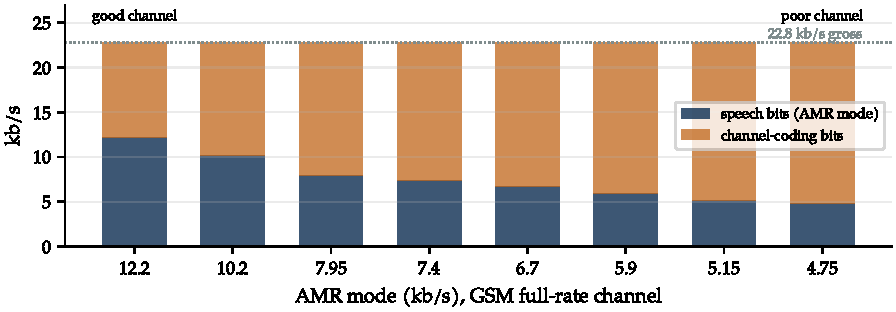
\includegraphics[width=0.92\linewidth]{figs/ch16_amr_modes}\caption{AMR's codec mode adaptation in a GSM full-rate channel. The gross rate is
fixed at 22.8\,kb/s; as the channel worsens the network moves to lower speech rates, and every
kilobit taken from the speech is given to the convolutional code. Speech quality falls a little, but
the call survives far deeper into the cell edge.}\label{fig:ch16_amr_modes}\end{figure}

Speech coding in mobile networks is shaped by the channel. The first digital cellular systems had
narrow, error-prone channels and needed codecs that were robust as well as efficient.
\begin{description}[style=nextline,leftmargin=1.2em,font=\sffamily\bfseries\small\color{navy}]
\item[GSM full rate (1990).] The RPE-LTP (regular-pulse excitation with long-term prediction) codec
at 13\,kb/s: LPC plus a pitch predictor, with a regular grid of pulses as the excitation, chosen
without a full analysis-by-synthesis search to fit the processors of the day. Its quality was
noticeably below wireline telephony.
\item[GSM enhanced full rate (1996).] A 12.2\,kb/s ACELP codec in the same channel gave
approximately wireline quality and was adopted quickly.
\item[AMR (1999).] The \term{adaptive multi-rate} codec (3GPP TS 26.090) has eight ACELP modes from
4.75 to 12.2\,kb/s (the 12.2 mode is the EFR codec). In GSM the gross channel rate is fixed at
22.8\,kb/s in a full-rate channel, and the network chooses the mode from measurements of channel
quality: in good conditions 12.2\,kb/s of speech and 10.6\,kb/s of convolutional coding; in poor
conditions 4.75\,kb/s of speech and the rest spent on stronger channel coding. This \emph{codec mode
adaptation} is a practical joint source--channel code (Section~\ref{sec:ch16:jscc}), and it extends
cell-edge coverage by several decibels (Figure~\ref{fig:ch16_amr_modes}). The speech bits of each mode are sorted into classes by their
perceptual sensitivity; the most important (class~1a) are protected by a CRC and the strongest code,
and a frame with a failed CRC is discarded and concealed by extrapolation from the previous one.
AMR is also the mandatory narrowband codec of UMTS.
\begin{figure}[H]\centering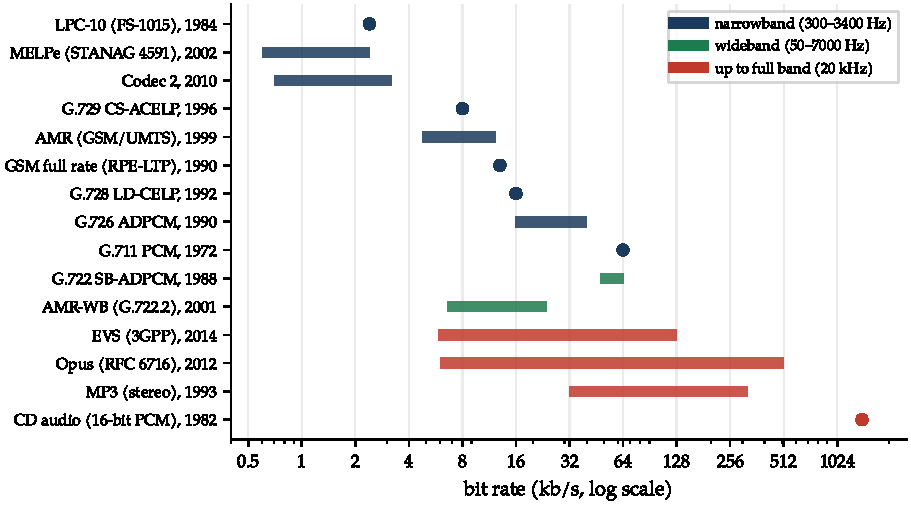
\includegraphics[width=0.85\linewidth]{figs/ch16_codecs}\caption{Bit rates of speech and audio codecs discussed in this chapter, coloured by
audio bandwidth, with the year of standardisation. Bars show the range of standard modes; dots mark
single-rate codecs. Over thirty years, the rate for telephone-quality narrowband speech fell from 64
to about 8\,kb/s, and then the effort switched to wider bandwidth and robustness rather than lower
rate.}\label{fig:ch16_codecs}\end{figure}

\item[AMR-WB (2001).] The wideband version (3GPP TS 26.190, identical to ITU-T G.722.2) samples at
16\,kHz, codes the 50--6400\,Hz band with ACELP and regenerates 6.4--7\,kHz from noise, at nine rates
from 6.6 to 23.85\,kb/s. It is the ``HD Voice'' of UMTS and LTE, and the improvement from adding the
band above 3.4\,kHz is dramatic: consonants such as \emph{s} and \emph{f}, which differ mostly above
3.4\,kHz, become distinguishable, and listening effort falls (Figure~\ref{fig:ch16_phone_band}).
\item[EVS (2014).] The \term{Enhanced Voice Services} codec (3GPP TS 26.441 and TS 26.445), designed
for VoLTE and carried into 5G voice, switches frame by frame between ACELP for speech and an MDCT
transform coder for music and noise, covers narrowband to full band (20\,kHz) at 5.9 to 128\,kb/s, and
includes a bit-exact AMR-WB interoperable mode. Its \emph{channel-aware mode} at 13.2\,kb/s sends a
compact redundant copy of important parameters of an earlier frame inside the current packet, so that
a lost packet can be partially reconstructed from a later one: forward error correction inside the
codec, tuned to the packet-loss rates of a loaded radio network.
\end{description}


\begin{inpractice}[Opus: the codec of the internet]
The \term{Opus} codec (IETF RFC~6716, 2012) is the dominant codec of interactive audio on the
internet: it is mandatory to implement in WebRTC (RFC~7874) and is used by browsers, many
conferencing and messaging applications, and game voice chat. Opus combines two very different
coders. \emph{SILK}, developed by Skype, is an LPC-based speech coder with noise-feedback quantisation,
used for speech up to wideband. \emph{CELT}, developed at Xiph.Org by Jean-Marc Valin and colleagues,
is a low-delay MDCT transform coder that codes the energy of each critical band explicitly and the
normalised band shape with pyramid vector quantisation, so that the spectral envelope is preserved
even at low rates. In \emph{hybrid} mode SILK codes the band below 8\,kHz and CELT the band above.
Opus runs from 6\,kb/s narrowband speech to 510\,kb/s stereo music, with frames from 2.5 to 60\,ms and
a default algorithmic delay of 26.5\,ms, and it can switch modes, bandwidth and rate at any frame
without signalling---an ideal match to a best-effort packet network whose capacity changes from
second to second. It includes in-band forward error correction (a low-rate copy of the previous
frame) and packet-loss concealment.
\end{inpractice}

Figure~\ref{fig:ch16_codecs} summarises the landscape. Two trends stand out. First, below about
8\,kb/s the quality of narrowband speech no longer improves much with rate; the effort since 2000 has
gone into bandwidth (wideband, super-wideband and full band) and into robustness to packet loss.
Second, the boundary between speech and audio coding has dissolved: EVS and Opus contain both an LPC
speech coder and an MDCT audio coder and switch between them, and the same is true of the MPEG USAC
(xHE-AAC) audio codec.

\mdcpairany{ch16_emodel}{The E-model's map from transmission rating $R$ to estimated MOS (ITU-T
G.107), with the user-satisfaction bands of ITU-T G.109. Each impairment---a low-rate codec, delay,
echo, packet loss---subtracts from $R$; the default with no impairments is 93.2.}{ch16_tandem}{Generation
loss, the image analogue of codec tandeming. Re-encoding the portrait with the same JPEG settings on
the same block grid barely changes it, but re-encoding with the grid shifted by 3 pixels each pass,
as when different codecs meet, loses about 4.5\,dB in eight passes.}

\subsection{Measuring speech quality}

How good is ``good''? Speech quality is ultimately a subjective matter, and it is measured
subjectively. In the \term{mean opinion score} (MOS) test of ITU-T P.800, panels of listeners rate
processed sentences on the absolute category rating scale---5 excellent, 4 good, 3 fair, 2 poor, 1
bad---and the scores are averaged. ``Toll quality,'' the quality of a good wireline call, corresponds
roughly to a MOS of 4 on this scale, but MOS values depend on the test conditions, the language and
the other systems in the test, so they should be compared only within one experiment.

Formal tests are slow and expensive, so objective models that predict MOS from the original and
degraded signals were developed and standardised: \term{PESQ} (ITU-T P.862, 2001) for narrowband and
wideband telephony, and its successor \term{POLQA} (ITU-T P.863, 2011), which also handles
super-wideband speech, time warping and the newer codecs. For network planning, the \emph{E-model} of
ITU-T G.107 combines impairments from the codec, delay, echo and packet loss into a single
transmission rating $R$ that maps to an estimated MOS (Figure~\ref{fig:ch16_emodel}).

\begin{pitfall}[Tandeming and non-speech signals]
A CELP codec models speech, and it does poorly on anything else. Music on hold turns watery;
fax and modem tones are destroyed, which is why networks must detect them and switch to G.711 or to a
relay protocol such as T.38; DTMF digits may be distorted enough to fail detection, so they are
normally carried out of band (RFC~4733 events). Worse is \emph{tandeming}: decoding and re-encoding the
speech at each network boundary. Each low-rate codec stage adds its own distortion, and two or three
tandems can lower quality noticeably (Figure~\ref{fig:ch16_tandem} shows the same effect for images).
Mobile networks therefore avoid transcoding whenever both ends support the same codec, with
tandem-free and transcoder-free operation (TFO, TrFO), and VoLTE calls between compatible handsets are
carried end to end without transcoding.
\end{pitfall}

%======================================================================
\mdcfig{ch16_noise_shaping}{Why a noisy MP3 sounds clean. Two noises of equal power are added to a
music frame. White noise (dashed) rises above the masking threshold over almost half of the band
(shaded) and is heard as hiss; the same power shaped to follow the threshold 6\,dB below it (green)
is completely hidden.}

\section{Perceptual audio coding}
\label{sec:ch16:audio}
%======================================================================

Here is a puzzle. A CD delivers 1411\,kb/s. An MP3 at 128\,kb/s keeps fewer than one bit in eleven,
and its signal-to-noise ratio, measured with a meter, is dreadful---often only a dozen or so
decibels in parts of the spectrum. Yet most people, on most music, cannot reliably tell the two
apart. How can a signal with so much noise sound clean?

Music has no source--filter model. A symphony orchestra, a distorted guitar and a rain shower have
nothing in common except the listener, and it is the listener that general audio codecs model. The
central fact is that the ear does not hear everything that reaches it: a loud sound hides quieter
sounds near it in frequency and time. A codec that puts its quantisation noise where it is hidden
can use far fewer bits than its SNR would suggest. That is the answer to the puzzle: the noise is
there, but it is hiding.

\begin{analogy}[A whisper during a drum hit]
Someone whispers to you just as the drummer hits the crash cymbal: you hear the cymbal, not the
whisper. Whisper again in a pause and you hear every word. The whisper did not change; the
\emph{context} did. A perceptual coder whispers its quantisation noise only where the music is
loud enough to drown it---next to strong tones, in busy frequency bands, in the instant after a
loud attack. The limit of the analogy: the hiding works only for sounds close in frequency and
time, so a loud bass note does nothing to hide a hiss at 10\,kHz.
\end{analogy}

\subsection{Psychoacoustics for the codec designer}

\subsubsection{The threshold in quiet}

The \term{absolute threshold of hearing}, the level of a pure tone that is just audible in silence,
depends strongly on frequency: it is lowest, around 0 to $-5$\,dB SPL, between 2 and 5\,kHz, where the
ear canal resonates, and rises steeply below 100\,Hz and above 15\,kHz
(Figure~\ref{fig:ch16_masking}a). A convenient fit due to Terhardt, with $f$ in kilohertz, is
\begin{equation}
T_q(f)=3.64f^{-0.8}-6.5\,e^{-0.6(f-3.3)^2}+10^{-3}f^4\quad\text{dB SPL}.
\label{eq:ch16:ath}
\end{equation}
A codec does not know how loud the listener will play the signal, so it assumes, conventionally, that a
full-scale sinusoid is reproduced at about 96\,dB SPL, which places the least significant bit of 16-bit
audio near the threshold.

\mdcfig{ch16_masking}{(a) The threshold in quiet~\eqref{eq:ch16:ath} and the masking thresholds
(dashed) of a tone and a narrow band of noise, computed with the Schroeder spreading function on the
Bark scale (top axis) and the tonal and noise offsets of Johnston's model. Their power sum with the
threshold in quiet is the global masking threshold (red). Noise masks more than a tone of the same
level, and masking spreads further towards high frequencies. (b) Temporal masking around a 200\,ms
masker (schematic, after Zwicker and Fastl): the threshold is raised for up to about 20\,ms before the
masker starts and 100--200\,ms after it stops.}

\subsubsection{Critical bands}

The cochlea acts as a bank of overlapping band-pass filters. Experiments on the detection of tones in
noise show that only noise within a certain bandwidth around a tone contributes to masking it; this
\term{critical bandwidth} is roughly 100\,Hz below 500\,Hz and about 20\% of the centre frequency above.
Counting critical bands from zero gives the \term{Bark} scale, after Heinrich Barkhausen, a
perceptual frequency axis on which the audible range spans about 24--25 Barks. A widely used
approximation, due to Zwicker, is
\begin{equation}
z(f)=13\arctan(0.00076f)+3.5\arctan\!\big((f/7500)^2\big)\ \text{Bark},\qquad f\text{ in Hz}.
\label{eq:ch16:bark}
\end{equation}
Half the Bark scale lies below about 1.7\,kHz (Figure~\ref{fig:ch16_bark}). The ear's frequency resolution is fine at low
frequencies and coarse at high ones, like a piano keyboard on which the keys get wider towards the
treble, and a codec's filterbank and bit allocation should follow suit.

\mdcfig[0.5]{ch16_bark}{The ear's frequency scale. The critical-band rate~\eqref{eq:ch16:bark}
(solid) rises quickly up to about 1\,kHz and slowly above; the critical bandwidth (dashed) is about
100\,Hz at low frequencies and grows to several kilohertz at the top of the audible range.}

\subsubsection{Simultaneous masking}

A \term{masker} raises the threshold of audibility of other sounds near it in frequency. On the Bark
scale the masking pattern has a roughly triangular shape: it falls steeply below the masker (about
25\,dB per Bark) and more gently above it (10 to 15\,dB per Bark, less for loud maskers), so that low
frequencies mask high ones more than the reverse (the \emph{upward spread of masking}). The peak of the
masking threshold lies some decibels below the masker, and here there is an important asymmetry:
noise is a much better masker than a tone. A noise band masks a tone at its centre to within about
5\,dB, whereas a tone masks noise only 15 to 25\,dB below its own level. Figure~\ref{fig:ch16_masking}(a)
shows the masking thresholds of a 70\,dB tone at 1\,kHz and a 60\,dB noise band at 4\,kHz computed with
a standard spreading function, and their combination with the threshold in quiet into a
\term{global masking threshold}. Anything below the red curve is inaudible, even though it may be only
20\,dB below a signal component and therefore far above the level that an SNR criterion would tolerate.

\subsubsection{Temporal masking}

Masking also extends in time (Figure~\ref{fig:ch16_masking}b). After a loud sound stops, the threshold
decays over 100 to 200\,ms (\emph{post-masking}, or forward masking). Remarkably, a loud sound also
masks sounds that occur a few milliseconds \emph{before} it (\emph{pre-masking}, or backward masking),
because the auditory system takes longer to process a quiet sound than a loud one. Pre-masking is
short, a few milliseconds and at most about 20\,ms, and that brevity creates the most notorious artefact
of transform audio coding, the pre-echo of Section~\ref{sec:ch16:preecho}.

\mdcfig[0.88]{ch16_psycho_frame}{A 46\,ms frame of a synthetic music signal---a harmonic tone at 220\,Hz and a band of noise
between 6 and 9\,kHz---with the masking threshold computed by a simplified psychoacoustic model
(tonal maskers identified as spectral peaks, noise maskers summed per critical band, spread with the
Schroeder function and added to the threshold in quiet). Everything in the shaded area is inaudible.
Only about 5\% of the spectral lines rise above the threshold, and even those need only enough
accuracy to keep the noise below the red curve.}

\begin{tryit}[Hide a tone]
Open Lab 24's \emph{Masking: hide a tone}. Leave the masker at 1\,kHz and 70\,dB SPL, put the
probe at 1400\,Hz, and lower \emph{Probe level} until the readout says the probe is inaudible;
press \emph{Listen} to check with your own ears. Now move the probe to 700\,Hz, the same distance
\emph{below} the masker: you will have to turn it much further down before it disappears. That is
the upward spread of masking.
\end{tryit}

\subsection{The perceptual coding principle}

A \term{perceptual audio coder} splits the signal into frequency components with a filterbank,
computes the masking threshold for each short frame with a \term{psychoacoustic model}, and
quantises each band just coarsely enough that the quantisation noise stays below the threshold.
The \term{signal-to-mask ratio} (SMR) in each band is the difference between the signal energy and the
masking threshold; the quantiser in that band must achieve an SNR of at least the SMR, which costs about
SMR/6.02 bits per sample in the band, and bands whose signal lies entirely below the threshold get
no bits at all (Figure~\ref{fig:ch16_band_bits}).

Figure~\ref{fig:ch16_psycho_frame} shows the idea on a synthetic frame. Only the strongest harmonics
of the tone rise above the masking threshold; the noise band and the upper harmonics lie entirely
below it and need not be coded at all---or, more precisely, need only be represented closely enough
that whatever the decoder substitutes is itself masked. James Johnston of Bell Labs formalised this
in 1988 as the \term{perceptual entropy}: the number of bits per sample needed to code each spectral
line with noise just at the masking threshold, $\sum_k\log_2(1+\sqrt{\text{SMR}_k})$ roughly. For the
frame of the figure a crude estimate gives about 190 bits, or about 8\,kb/s for this simple mono
signal. For real music, perceptual entropies are typically a small fraction of the 16 bits per sample
of the CD, which is why coders reach transparency for most material at 1.5--2 bits per sample
(roughly 128--192\,kb/s for stereo).

\mdcfig[0.9]{ch16_band_bits}{Bit allocation for the frame of Figure~\ref{fig:ch16_psycho_frame},
band by band. Navy bars: the signal-to-mask ratio in each critical band; red: the bits per spectral
line needed to keep the quantisation noise under the mask, about SMR/6 at the worst line of the
band. Eleven of the 25 bands, including the whole noise band at the top, need no bits at all, and
none needs more than about 3.5---a far cry from the 16 bits of the CD.}

The same accounting explains the puzzle we started with. Figure~\ref{fig:ch16_noise_shaping} adds
noise of exactly the same total power to the frame in two ways. Spread evenly across the spectrum
(white), it pokes above the threshold over half the band and is clearly audible. Shaped to sit 6\,dB
under the threshold everywhere, it is inaudible. Same SNR, opposite verdicts: the meter measures
power, the ear measures power \emph{relative to the mask}.

\begin{tryit}[Hear the noise you cannot hear]
In Lab 24's \emph{Noise under the mask}, set \emph{Noise} to \emph{Shaped under the mask} and
\emph{Noise relative to the threshold} to $-6$\,dB, and listen: music alone, then music plus noise.
Note the SNR readout. Now switch to \emph{White, same power} without touching anything else and
listen again---same SNR, audible hiss. Finally raise the shaped noise to $+6$\,dB and watch the
\emph{Bands with audible noise} readout leave zero.
\end{tryit}

\subsection{Filterbanks and the MDCT}

A perceptual coder needs a filterbank with good frequency resolution (to follow the critical bands
and to concentrate tonal energy in few coefficients), critical sampling (as many coefficients as input
samples, or the rate grows), perfect reconstruction in the absence of quantisation, and overlapping
windows (so that quantisation noise does not produce audible discontinuities at block boundaries). A
plain block DCT fails the last requirement; the \term{modified discrete cosine transform} (MDCT) meets
them all.

\subsubsection{The MDCT and time-domain aliasing cancellation}

The MDCT maps a block of $2N$ windowed input samples to $N$ coefficients,
\begin{equation}
X[k]=\sum_{n=0}^{2N-1}w[n]\,x[n]\cos\!\Big[\frac{\pi}{N}\Big(n+\frac12+\frac N2\Big)\Big(k+\frac12\Big)\Big],\qquad k=0,\dots,N-1,
\label{eq:ch16:mdct}
\end{equation}
and successive blocks overlap by $N$ samples, so the transform is critically sampled: $N$ new samples
in, $N$ coefficients out. That sounds impossible---half as many outputs as inputs in each block---and
indeed a single block cannot be inverted. The magic happens between neighbours.


\mdcfig{ch16_mdct}{(a) Sine windows overlapped by 50\%, satisfying the Princen--Bradley condition. (b)
The inverse MDCT of each block (coloured) contains time-reversed aliases; overlap-adding neighbours
cancels them and reconstructs the input exactly (dashed over grey). (c) Pre-echo. A quiet tone is
followed at 68\,ms by a sharp attack. Coding each block at the same SNR spreads the quantisation noise
uniformly over the window: with 2048-sample windows (46\,ms) the noise starts some 20\,ms before the
attack, where nothing masks it; with 256-sample windows it is confined to a few milliseconds and hidden
by pre-masking.}

\begin{deeper}[How the aliases cancel]
The inverse transform, $y[n]=\frac2N\,w[n]\sum_kX[k]\cos[\cdot]$, returns the windowed input
\emph{plus a time-reversed alias} of it in each half of the block, with opposite signs in the two
halves. When the window satisfies the \term{Princen--Bradley condition}
\begin{equation}
w^2[n]+w^2[n+N]=1,\qquad n=0,\dots,N-1,
\label{eq:ch16:pb}
\end{equation}
as the sine window $w[n]=\sin[\pi(n+\frac12)/2N]$ does, the alias in the second half of one block
exactly cancels the alias in the first half of the next when the outputs are overlapped and added.
This \term{time-domain aliasing cancellation} (TDAC), found by John Princen and Alan Bradley in 1986,
is the frequency-domain dual of the aliasing cancellation in a quadrature-mirror filterbank
(Chapter~\ref{ch:dsp}).
\end{deeper}

Figure~\ref{fig:ch16_mdct}(b) shows TDAC happening: each block's output is badly distorted, and the
sum is exact to machine precision. The MDCT can be computed with an FFT of size $N/2$, and it is the
transform of AAC, Dolby AC-3, Vorbis, Opus's CELT layer, the transform mode of EVS, and the hybrid
filterbank of MP3.

\subsubsection{Pre-echo and block switching}
\label{sec:ch16:preecho}

Long windows give fine frequency resolution: a 2048-sample window at 44.1\,kHz resolves 21.5\,Hz,
ideal for tonal music. But quantisation noise added to the coefficients spreads over the whole window
after the inverse transform. If a sharp attack---castanets, a snare drum, a plucked string---occurs
near the end of the window, the noise appears before the attack, in a quiet interval where pre-masking
lasts only a few milliseconds (Figure~\ref{fig:ch16_mdct}c). The result, a smeared ``pre-echo'' before
each transient, was the most audible defect of early transform coders. The remedy is \term{block
switching}: when a detector finds a transient, the coder switches to short windows (in AAC, eight
windows of 256 samples in place of one of 2048), using asymmetric transition windows that preserve the
Princen--Bradley condition. AAC adds \term{temporal noise shaping} (TNS), which applies linear
prediction \emph{across frequency} to the MDCT coefficients; by the duality of time and frequency, this
shapes the quantisation noise in time to follow the signal envelope within the block. Both tools trade
a few bits for the removal of a highly objectionable artefact.

\begin{figure}[H]\centering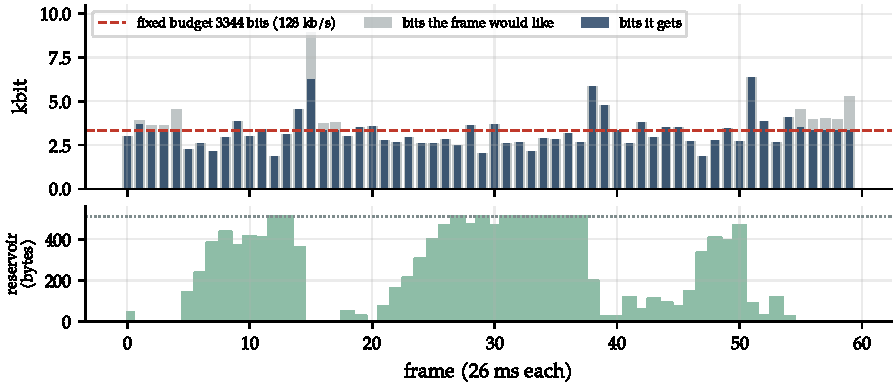
\includegraphics[width=0.9\linewidth]{figs/ch16_bit_reservoir}\caption{The bit reservoir as a savings account (simulated). At 128\,kb/s a
44.1\,kHz MP3 frame has a budget of 3344 bits (dashed). Quiet frames need less and bank the
difference, up to 511 bytes (bottom); transients such as frames 14--15 and 51 then draw on the savings
and get far more than the budget. Only when the reservoir is empty is a frame short-changed (grey
tops).}\label{fig:ch16_bit_reservoir}\end{figure}

\subsection{MP3 and AAC}

\subsubsection{MPEG-1 Layer III}

The MPEG-1 audio standard (ISO/IEC 11172-3, finalised in 1992) defined three layers of increasing
complexity. Layers I and II use a 32-band polyphase quadrature-mirror filterbank with block-companded
quantisation in each band; Layer II (MP2) is still the audio codec of DAB digital radio and of many
DVB broadcasts. Layer III, \term{MP3}, adds much more machinery:
\begin{itemize}[nosep]
\item a \emph{hybrid filterbank}: the 32 polyphase subbands are each split further by an 18-point MDCT,
giving 576 frequency lines per \emph{granule}, two granules per 1152-sample frame, with switching to
three short 6-point transforms per subband for transients;
\item non-uniform quantisation with a power law, $\hat X=\operatorname{sgn}(X)|X|^{3/4}$ before rounding,
which gives larger values larger steps;
\item scale factors per band, chosen by an iterative \emph{analysis-by-synthesis} loop in which an inner
loop adjusts the global step until the frame fits the bit budget and an outer loop amplifies the bands
whose noise exceeds the masking threshold;
\item Huffman coding of the quantised lines with a set of tables selected per region of the spectrum;
\item joint stereo: mid/side coding of $L+R$ and $L-R$ when the channels are similar, and intensity
stereo, which sends a single channel plus direction information at high frequencies;
\item a \term{bit reservoir}: frames are nominally of fixed size for a constant bit rate, but a frame may
borrow bits left unused by earlier frames (up to 511 bytes back). Easy frames donate bits to difficult
ones, so the coder behaves like a variable-rate coder with a small buffer while the channel sees a
constant rate (Figure~\ref{fig:ch16_bit_reservoir}).
\end{itemize}

At 128\,kb/s for stereo---about 11:1 compression from the CD rate---MP3 is good enough for most
listeners on most material, and at 192--256\,kb/s nearly transparent.

\mdcfig{ch16_sbr}{Spectral band replication. (a) A synthetic chord with harmonics to 19\,kHz. (b) A core
codec at low rate keeps only the band below 8\,kHz: the result sounds muffled. (c) The SBR decoder copies
the 4--8\,kHz band upwards and rescales it, band by band, to the original's coarse envelope, sent as a
few kilobits per second of side information. The harmonics in the rebuilt band are in the wrong places,
but the ear, judging mostly the envelope up there, rarely notices.}

\subsubsection{AAC and its extensions}

\term{Advanced Audio Coding} (AAC), standardised in MPEG-2 (1997) and extended in MPEG-4, removes the
compromises MP3 inherited from its Layer I/II compatibility. It uses a pure MDCT with 2048-sample
windows (1024 lines) switching to eight 256-sample windows, a choice of sine or Kaiser--Bessel-derived
window shapes, TNS, flexible mid/side and intensity stereo, better Huffman coding of scale factors and
spectral data, and up to 48 channels. In formal listening tests AAC generally reached the quality of
MP3 at a noticeably lower bit rate, and AAC became the codec of the iTunes store, of YouTube and most
streaming services, of digital television (in DVB and ISDB) and of the soundtrack of nearly every
video file.

At low rates even AAC runs out of bits for the top octave, and simply low-pass filtering the audio
makes it sound dull. \term{Spectral band replication} (SBR), developed by Coding Technologies in Sweden
and standardised as \emph{HE-AAC} (MPEG-4, 2003), codes only the lower half of the spectrum with the core
AAC coder, at half the sampling rate, and \emph{regenerates} the upper half at the decoder by
transposing the low band upwards and shaping its envelope with a few kilobits per second of side
information (spectral envelope, tonality and noise-floor parameters;
Figure~\ref{fig:ch16_sbr}). Because the ear is much less sensitive to the fine structure of high
frequencies than to their envelope, the result sounds full-bandwidth.

\emph{Parametric stereo} (PS), added in HE-AAC~v2 (2006), goes further: it sends a mono downmix and a
few parameters per band (inter-channel level and phase differences and coherence) from which the
decoder recreates a stereo image. HE-AAC~v2 delivers acceptable stereo at 24--48\,kb/s and is the codec
of DAB+ digital radio and of Digital Radio Mondiale on the short-wave bands, where every kilobit per
second is precious. The MPEG-D USAC codec (2012), marketed as xHE-AAC, merges AAC with an ACELP speech
coder and improved SBR and stereo tools, and works from about 6\,kb/s upwards for both speech and
music.

\mdcpairany{ch16_brandenburg}{Karlheinz Brandenburg, whose doctoral work at Erlangen and team at
Fraunhofer IIS produced much of MP3.}{ch16_vega}{Suzanne Vega in concert. Her unaccompanied
recording of ``Tom's Diner'' (1987) became, by Brandenburg's own account, the test track that
exposed the early coder's flaws---a lone voice leaves no music to hide the noise under.}

\begin{history}[The MP3 story]
Karlheinz Brandenburg (Figure~\ref{fig:ch16_brandenburg}) began working on perceptual audio coding for his doctoral thesis at the
University of Erlangen-Nuremberg in the 1980s, in a project whose original goal was to send music over
ISDN telephone lines at 64 or 128\,kb/s. With colleagues at the Fraunhofer Institute for Integrated
Circuits (IIS) in Erlangen and partners at AT\&T Bell Labs, Thomson and elsewhere, his group developed
the ASPEC coder, which contributed the core of MPEG-1 Layer III. Brandenburg has described tuning the
coder on Suzanne Vega's a cappella recording of ``Tom's Diner'' (Figure~\ref{fig:ch16_vega}), whose unaccompanied voice exposed every
artefact and which he listened to hundreds of times. Layer III was standardised in 1992 but initially
lost out to the simpler Layer II in broadcasting. Its breakthrough came from personal computers:
Fraunhofer's encoder and the \texttt{.mp3} file extension (chosen in 1995), a free player, portable players (Figures~\ref{fig:ch16_rio} and~\ref{fig:ch16_ipod}), the rise of
the internet and then Napster in 1999 turned a telecommunications research project into a force that
reshaped the recorded-music industry. The MP3 patents expired around 2017, and Fraunhofer ended its
licensing programme that year, by which time AAC had largely replaced it.
\end{history}

\mdcpairany{ch16_rio}{The Diamond Rio PMP300 (1998), one of the first portable MP3 players: 32\,MB of
flash memory, about half an hour of music at 128\,kb/s.}{ch16_ipod}{An Apple iPod classic (2007
generation). With a hard disk and AAC as well as MP3, players like this put thousands of songs in a
pocket; compression, not storage, made the music library portable.}

\begin{inpractice}[MiniDisc and ATRAC]
MP3 was not the first perceptual coder in consumers' hands. Sony's MiniDisc (1992, Figure~\ref{fig:ch16_minidisc}) recorded on a
small magneto-optical disc in a cartridge, and fitted the 74 minutes of a CD on it with ATRAC
(Adaptive TRansform Acoustic Coding), a perceptual coder that split the signal into three subbands
with quadrature-mirror filters and coded each with an MDCT of adaptive length, reducing the
1.4\,Mb/s of CD audio to about 292\,kb/s---a ratio of roughly five. Later ATRAC versions squeezed two
and four times as much music onto the same disc. The format's arc---from a dedicated consumer
format to ubiquitous files on general-purpose players---previewed what would happen to MP3 and AAC.
\end{inpractice}

\mdcphoto[0.45]{ch16_minidisc}{A MiniDisc with its cartridge opened, showing the 64\,mm
magneto-optical disc. Its ATRAC coder brought perceptual audio coding to consumers in 1992.}

\begin{inpractice}[Audio codecs in broadcasting]
Broadcast audio is a catalogue of this section's history. DAB (Eureka-147, 1995) uses MPEG-1 Layer II at
typically 128--192\,kb/s per stereo programme; DAB+ (2007) switched to HE-AAC~v2 and fits roughly three
times as many stations in the same multiplex. DVB television uses MPEG-1 Layer II, AAC, HE-AAC and Dolby
codecs. \term{Dolby AC-3} (Dolby Digital), introduced in cinemas in 1992 and standardised for US digital
television as ATSC A/52, is an MDCT coder with 512-sample windows and an exponent--mantissa
(floating-point-like) coefficient representation; it carries 5.1 channels in 384--448\,kb/s on DVD and
ATSC~1.0. ATSC~3.0 and newer DVB services use Dolby AC-4 or MPEG-H 3D Audio, which add object-based
audio (sounds sent as objects with positions rather than as fixed speaker channels) and dialogue
enhancement. HD Radio (NRSC-5) uses a proprietary perceptual codec (HDC) at a few tens of kilobits per
second per programme.
\end{inpractice}

\subsection{Lossless audio}

Archiving, mastering and a growing share of music streaming use \emph{lossless} coding. The
dominant format, \term{FLAC} (Free Lossless Audio Codec, released by Josh Coalson in 2001), is a direct
application of Sections~\ref{sec:ch16:lossless} and~\ref{sec:ch16:lpc}: each block of a few thousand
samples is predicted with a fixed polynomial predictor or an LPC filter of order up to 32 (with
quantised coefficients sent in the header), inter-channel correlation is removed with mid/side
decorrelation, and the integer residual is Rice coded with the parameter adapted per partition of the
block. Because prediction is done in integer arithmetic on the original samples, decoding is exact.

\mdcphoto[0.45]{ch16_cd}{A compact disc. Its 1411\,kb/s of 16-bit stereo PCM is the reference
against which every audio codec is judged; a lossless coder such as FLAC typically halves it, a
perceptual coder divides it by ten.}

Typical CD audio (Figure~\ref{fig:ch16_cd}) compresses to around 50--70\% of its original size, depending heavily on the music:
quiet acoustic recordings compress well, dense, loud modern masters much less. Apple's ALAC and MPEG-4
ALS work the same way. Lossless coding also illustrates the entropy limit of
Chapter~\ref{ch:infotheory} directly: no lossless coder can remove the noise floor of the recording,
which is incompressible, and for a 16-bit recording with a noise floor several bits above the least
significant bit those noisy bits set a hard floor on the compressed size. That is why the lossless
saving on a CD is a factor of about two and no more, while a perceptual coder, free to discard the
noise floor because nobody can hear it, gains a factor of ten.

%======================================================================
\section{Image coding}
\label{sec:ch16:image}
%======================================================================

Your phone's camera captures twelve million pixels, three colours each: 36 megabytes of raw data
per photo. The JPEG it saves is three or four megabytes, and you would struggle to spot the
difference. A photograph is a two-dimensional signal with strong local correlation, sharp edges,
textures, and a consumer---the human visual system---that is more forgiving of some errors than
others. Still-image coding is also where the transform-coding recipe of
Section~\ref{sec:ch16:lossy} was first put into mass production, and every video codec reuses its
machinery for the pictures it codes without reference to others.

\subsection{Colour and chroma subsampling}

Cameras and displays work in red, green and blue, but the three RGB planes of a natural image are
highly correlated, and the eye's sensitivity to fine detail is concentrated in brightness rather than
colour. (Look at a colour photo in dim light: you still see every edge, but the colours fade.) Image
and video codecs therefore convert to a luma--chroma space. The \term{YCbCr} transform of
ITU-R BT.601, used by JPEG, is
\begin{equation}
\begin{aligned}
Y&=0.299R+0.587G+0.114B,\\
C_b&=128+0.564\,(B-Y),\qquad C_r=128+0.713\,(R-Y),
\end{aligned}
\label{eq:ch16:ycbcr}
\end{equation}
where the luma weights follow the eye's spectral sensitivity---green counts most, blue least;
high-definition video uses the slightly different weights of BT.709 and ultra-high-definition those
of BT.2020. The chroma planes are smooth and low in energy (Figure~\ref{fig:ch16_chroma}), and the
visual system resolves colour detail at roughly half or less of the resolution at which it resolves
luminance detail.

\mdcfig{ch16_chroma}{A colour image and its luma and chroma planes. The chroma planes carry little
detail. The right-hand image was rebuilt with chroma downsampled by four in each direction---one
chroma sample per 16 pixels, four times coarser than 4:2:0---and upsampled again; it is hard to tell
from the original, although its RGB PSNR is only 33\,dB.}

Codecs exploit this with \term{chroma subsampling} (Figure~\ref{fig:ch16_chroma_formats}): in
\emph{4:2:2} format the chroma planes have half the horizontal resolution of luma, and in
\emph{4:2:0}, the format of almost all consumer images and video, half the resolution in both
directions. 4:2:0 halves the raw data (12 bits per pixel instead of 24) before any coding, at a
cost that is invisible in natural images and noticeable only in sharp coloured text and graphics.

\begin{figure}[htbp]\centering
\begin{tikzpicture}[x=0.42cm,y=0.42cm]
\foreach \fmt/\xo/\sx/\sy/\name in {0/0/1/1/{4:4:4},1/9.5/2/1/{4:2:2},2/19/2/2/{4:2:0}} {
  \foreach \i in {0,...,3} \foreach \j in {0,...,3}
    \draw[navy!60,fill=navy!8] (\xo+\i*1.6,\j*1.6) rectangle ++(1.3,1.3);
  \foreach \i in {0,...,3} \foreach \j in {0,...,3} {
    \pgfmathsetmacro{\ok}{(mod(\i,\sx)==0 && mod(\j,\sy)==0) ? 1 : 0}
    \ifdim\ok pt>0.5pt
      \fill[accent] (\xo+\i*1.6+0.65+0.8*\sx-0.8,\j*1.6+0.65+0.8*\sy-0.8) circle (0.28);
    \fi}
  \node[font=\sffamily\small\bfseries,text=navy] at (\xo+3.0,-1.0) {\name};
}
\node[font=\sffamily\scriptsize,anchor=west] at (28.5,4.6) {\textcolor{navy!60}{$\blacksquare$} luma sample (Y)};
\node[font=\sffamily\scriptsize,anchor=west] at (28.5,3.4) {\textcolor{accent}{$\bullet$} chroma pair (Cb, Cr)};
\node[font=\sffamily\scriptsize,anchor=west,align=left] at (28.5,1.6) {raw bits per pixel:\\4:4:4 = 24, 4:2:2 = 16,\\4:2:0 = 12};
\end{tikzpicture}
\caption{Chroma subsampling formats. Every pixel keeps its own brightness sample (squares), but in
4:2:2 two horizontally adjacent pixels share one colour sample (dot) and in 4:2:0 a $2\times2$ group
does. Studio video uses 4:2:2; almost everything you watch or photograph is 4:2:0.}
\label{fig:ch16_chroma_formats}
\end{figure}

Colour conversion hides one more subtlety. Pixel values are not proportional to light intensity: they
are \emph{gamma-encoded}, roughly as the 0.45 power of intensity, which approximates the eye's roughly
logarithmic response to brightness and so spreads the quantisation levels perceptually evenly. Coding
is done on the gamma-encoded values, which is one reason why mean-squared error in pixel values is at
least a reasonable first approximation to visible error.

\subsection{JPEG}

The baseline \term{JPEG} codec (ITU-T T.81, ISO/IEC 10918-1) processes each colour component
independently, in $8\times8$ blocks:
\begin{enumerate}[nosep]
\item \textbf{Level shift and DCT.} Subtract 128 from each 8-bit pixel and take the two-dimensional
DCT~\eqref{eq:ch16:dct} (separable: rows, then columns). The DC coefficient is eight times the block
mean; the 63 AC coefficients describe the detail (Figure~\ref{fig:ch16_dct_basis}).
\item \textbf{Quantisation.} Divide each coefficient by the corresponding entry of an $8\times8$
\term{quantisation table} and round. The tables in Annex~K of the standard were derived from
visibility experiments: steps are small (10--16) for low frequencies and large (up to 121) for high
frequencies, and larger for chroma than for luma. Encoders scale the table with a single ``quality''
parameter $Q$ from 1 to 100; in the widely used IJG convention, $Q=50$ gives the Annex~K table itself,
lower $Q$ scales it up and higher $Q$ down. This is the only lossy step, and it is where JPEG is
perceptual: the table is a crude contrast-sensitivity model.
\item \textbf{Zigzag scan.} Reorder the 64 quantised coefficients from low to high frequency along the
zigzag path (Figure~\ref{fig:ch16_jpeg_block}c), which tends to group the nonzero values at the start
and leave a long tail of zeros.
\item \textbf{DC coding.} Code the DC coefficient as the difference from the previous block's DC
(a DPCM step), as a \emph{size category} (the number of bits needed for the value) that is Huffman
coded, followed by that many bits giving the value.
\item \textbf{AC coding.} Code each nonzero AC coefficient as a Huffman-coded pair (\emph{run},
\emph{size})---the number of zeros that precede it and its size category---followed by the value bits.
Special symbols code a run of 16 zeros (ZRL) and \emph{end of block} (EOB) after the last nonzero
coefficient.
\end{enumerate}
The decoder reverses the steps, multiplying each index by its step size and taking the inverse DCT.
Figure~\ref{fig:ch16_jpeg_block} follows one real block through the pipeline, and the worked example
counts its bits.

\mdcfig{ch16_jpeg_block}{One $8\times8$ luma block from the portrait (the red square in
Figure~\ref{fig:ch16_jpeg_quality}, on the chin and lower lip) through the JPEG pipeline at $Q=50$. (a)
Pixel values. (b) DCT coefficients: the energy is concentrated in the first column, because the block
contains a horizontal edge (bright skin above, dark below). (c) The coefficients divided by the
Annex~K table and rounded: only 12 of 64 are nonzero; the orange line is the zigzag scan. (d) The
decoded block. The RMS error is 6.4 grey levels.}

\begin{worked}[Coding a real JPEG block]
Take the block of Figure~\ref{fig:ch16_jpeg_block} and assume it is the first block of the image, so the
DC predictor is zero. The quantised values in zigzag order are
\[
14\ \big|\ 3,\ 17,\ -15,\ 2,\ 2,\ -1,\ 1,\ 0,\ 5,\ -1,\ \underbrace{0,\dots,0}_{7},\ 1,\ \underbrace{0,0,0,0}_{4},\ 1,\ 0,\dots
\]
\emph{DC.} The value 14 is in size category 4 (values 8--15). With the example luminance DC table of
Annex~K, category 4 has the codeword \texttt{101}, followed by the four bits \texttt{1110}: 7 bits.

\emph{AC.} The symbols are (0,2)\,3; (0,5)\,17; (0,4)\,$-15$; (0,2)\,2; (0,2)\,2; (0,1)\,$-1$; (0,1)\,1;
(1,3)\,5; (0,1)\,$-1$; (7,1)\,1; (4,1)\,1; EOB. The example AC luminance table gives codeword lengths of 2
bits for (0,1) and (0,2), 4 for (0,4), 5 for (0,5), 7 for (1,3), 6 for (4,1), 8 for (7,1) and 4 for EOB.
Adding the value bits (equal to the size category) gives
\[
3(2+2)+(5+5)+(4+4)+3(2+1)+(7+3)+(8+1)+(6+1)+4=69\ \text{bits}.
\]
The block costs $7+69=76$ bits instead of $64\times8=512$: a compression ratio of 6.7:1, or 1.19 bits
per pixel, with a PSNR for the block of $20\log_{10}(255/6.42)=32.0$\,dB. This is a busy block with a
strong edge; smooth blocks of skin or background cost 10--20 bits, and averaged over the whole image
the same settings give 0.90 bits per pixel, a ratio of 8.9:1 (Figure~\ref{fig:ch16_jpeg_quality}).
Notice where the bits went: 28 bits for the three large AC coefficients (17, $-15$ and 5) that describe
the edge, 16 bits for the two isolated $\pm1$ values late in the scan, and only 4 bits to say that the
remaining 40 coefficients are all zero. That last number is the power of the EOB symbol and the zigzag scan.
\end{worked}

\mdcfig{ch16_jpeg_quality}{The chapter's JPEG implementation (baseline JPEG with IJG quality scaling
and optimised Huffman tables, headers not counted) at three quality settings, with the bit rate in bits
per pixel and the PSNR. At $Q=50$ the image is visually indistinguishable from the original at this size;
at $Q=15$ smooth areas begin to show blocks; at $Q=4$ most blocks are reduced to their DC value and a
few AC coefficients, and the $8\times8$ grid is plain to see.}

\begin{tryit}[Turn the quality knob]
In Lab 24's \emph{A toy JPEG}, start at \emph{Quality} 50 on the \emph{Photograph} and drag it down
slowly, watching the decoded image, the bits-per-pixel readout and the PSNR. Find the setting at
which blocks first become visible to you---note its PSNR---then set \emph{Right-hand view} to
\emph{Error $\times$4} to see where the bits were taken away. Can you get below 1 bit per pixel
while keeping the PSNR above 32\,dB?
\end{tryit}

\subsubsection{Artefacts and what JPEG leaves on the table}

At high compression JPEG produces two characteristic artefacts (Figure~\ref{fig:ch16_jpeg_zoom}).
\term{Blocking} appears because each block is coded independently: when a smooth gradient is
reduced to a single DC value per block, the block boundaries become visible steps. \term{Ringing}
appears around sharp edges, because the discarded high-frequency coefficients leave Gibbs-like
oscillations inside the block. Decoders can hide some of both with post-filters, and later codecs
build a \emph{deblocking filter} into the prediction loop (Section~\ref{sec:ch16:video}).

\mdcfig{ch16_jpeg_zoom}{JPEG artefacts up close: the portrait at quality 8 (0.28 bits per pixel,
a 28:1 ratio). The face has become a mosaic of $8\times8$ tiles (blocking), and the error map shows
the damage concentrated along edges and textures---the eyebrows, the creases, the collar---with
ringing inside the blocks that straddle them. Flat skin, which needed only its DC value, is almost
untouched.}

Have you noticed that streaming video looks worst in dark scenes---a night sky or a shadowy room
breaking into blotchy blocks while bright daylight scenes look fine? The same mechanism is at work
(Figure~\ref{fig:ch16_dark_scene}). Dark scenes are usually smooth and low in contrast: their gentle
gradients put almost all of each block's energy into the DC coefficient, the AC coefficients
quantise to zero, and each block becomes flat. Where the gradient is shallow, the step from one
block's DC level to the next is larger than the change inside the block, and you see a staircase of
tiles. Your eyes make matters worse: adapted to a dark room, they are sensitive to small steps in
dim regions, and the noise that would otherwise dither the steps is often removed by the encoder's
denoiser because it costs bits. Modern encoders fight back with adaptive quantisation that spends
extra bits on flat dark areas, with 10-bit coding, and with deliberately added film grain
(Section~\ref{sec:ch16:video}).

JPEG also leaves efficiency on the table: the DC prediction uses only the previous block, the Huffman
coding is not adaptive and the $8\times8$ block size is fixed. Its arithmetic-coding and progressive
modes fix some of this but were rarely implemented. Modern JPEG encoders (for example Google's
\emph{guetzli} and \emph{jpegli}, and Mozilla's \emph{mozjpeg}) wring out substantial savings by
optimising the quantisation and coefficient decisions while remaining decodable by any standard
decoder---an example of the rule that a standard defines only the decoder, leaving encoders free to
improve for decades.

\mdcfig{ch16_dark_scene}{Why video blocks up in dark scenes. Two gentle gradients, one dark and one
bright, both coded with the toy JPEG at the same quality. The dark one (shown six times brighter so
you can see what a dark-adapted eye sees) collapses into flat blocks with visible steps between them;
the row profile on the right is a staircase. The bright gradient's larger slope survives as
smaller steps that are hard to see.}

\begin{history}[The JPEG committee]
In the mid-1980s several groups within ISO and the CCITT (now ITU-T) were studying the compression of
photographic images for videotex, facsimile and the new personal computers. In 1986 they formed a
joint group, the \emph{Joint Photographic Experts Group}. The group ran a competition among a dozen
proposed techniques, and in 1988 an adaptive DCT scheme was selected over rival predictive and
block-truncation methods after subjective tests of the candidate coders on a set of standard test
images. The specification was approved as ITU-T T.81 in 1992 and as ISO/IEC 10918-1 in 1994. The
standard itself did not define a file format; the de facto JFIF format (1992) and the free software
library of the Independent JPEG Group (first released in 1991) did as much to spread JPEG as the
standard did, and the Exif format of digital cameras carried it into every phone. More than three
decades later, baseline JPEG remains the most widely used image format in the world---a testament to
getting the essentials right and keeping them simple.
\end{history}

\subsection{JPEG 2000 and wavelets}

The block DCT treats an image as a set of independent tiles. The \term{discrete wavelet transform}
(DWT) treats it as a hierarchy of scales, like a set of maps of the same country at different zoom
levels. One level of a 2D wavelet transform filters the image with a low-pass/high-pass pair along
rows and along columns and downsamples by two in each direction, producing a quarter-size
approximation (LL) and three detail subbands (LH, HL, HH) that capture horizontal, vertical and
diagonal edges. Repeating on LL gives a multi-resolution pyramid (Figure~\ref{fig:ch16_wavelet}).
The filters are short and overlapping, so there are no block boundaries and hence no blocking
artefacts, and the detail coefficients are sparse: most are near zero, with large values only along
edges.

\mdcfig{ch16_wavelet}{(a) A three-level wavelet decomposition of the portrait with the reversible
LeGall 5/3 filters of JPEG~2000, implemented by lifting; detail subbands are amplified by four. The
coarsest approximation (top left, $32\times32$) is a thumbnail of the image; the detail subbands are
mostly grey (near zero) except along edges. (b) Histograms of the pixel values and of the finest
diagonal subband on a log scale. The detail coefficients are sharply peaked at zero: the finest
subbands each hold only 2--5\% of the pixel variance, and most of their coefficients quantise to zero.}

\term{JPEG~2000} (ISO/IEC 15444-1, ITU-T T.800, 2000) combines a wavelet transform with an
embedded entropy coder, EBCOT (embedded block coding with optimised truncation), invented by David
Taubman. It uses the LeGall 5/3 filters, implemented by \emph{lifting} with integer arithmetic, for
lossless coding, and the Cohen--Daubechies--Feauveau 9/7 filters for lossy coding. Each subband is
divided into code blocks (typically $64\times64$) whose coefficients are coded bit plane by bit plane,
from the most significant, with the context-adaptive MQ arithmetic coder. Because each bit plane
refines the previous one, the compressed stream is \emph{embedded}: truncating it anywhere gives the
best image for that number of bits. A single file can therefore be decoded at many rates, resolutions
and qualities, and regions of interest can be given priority.

JPEG~2000 gives better quality than JPEG at the same rate, especially at low rates where JPEG blocks,
and its scalability and lossless mode are unique, but it never displaced JPEG on the web or in cameras:
the gain at typical web qualities was modest, decoding was several times slower, and JPEG was already
everywhere. It found its homes where its features matter: \emph{digital cinema} (the DCI specification
codes every frame of a theatrical feature as a JPEG~2000 image at up to 250\,Mb/s), medical imaging
(DICOM), archives and geospatial imagery, and broadcast contribution links.

\subsection{Lossless images: PNG and friends}
\label{sec:ch16:png}

\term{PNG} (Portable Network Graphics, 1996; RFC~2083) codes images losslessly by combining a simple
predictor with DEFLATE. Each row is first transformed by one of five \emph{filters}---None, Sub (predict
from the left neighbour), Up (from above), Average (of left and above) and Paeth (whichever of left,
above and upper-left is closest to the linear estimate left${}+{}$above${}-{}$upper-left)---chosen per row
by the encoder, and the filtered bytes are then DEFLATE-compressed (Figure~\ref{fig:ch16_png_filters}).

PNG excels on graphics, screenshots and text, where the LZ77 stage finds long repeated strings, and
it is poor on photographs: our portrait needs 5.2 bits per pixel losslessly, against about 1 bit per
pixel for a visually excellent lossy JPEG. That factor of five is the cost of insisting on
reproducing the camera's noise exactly. JPEG-LS (based on HP Labs' LOCO-I predictor with context
modelling and Golomb coding) and lossless JPEG~XL do better on photographs, but not dramatically:
noise is incompressible. Notice, too, how close the figure's simple order-0 entropy after the Paeth
filter (5.13 bits) is to what PNG actually achieves (5.18 bits): on a photograph, DEFLATE's
dictionary finds almost nothing to reuse, and the gain comes almost entirely from the prediction
filter.

\mdcfig[0.55]{ch16_png_filters}{What PNG's filters do to the portrait. Raw pixel bytes (grey) are
spread over the whole range, with an order-0 entropy of 7.13 bits; after the Sub filter (orange)
they pile up around zero at 5.42 bits, and the Paeth filter (navy) does slightly better at 5.13
bits. DEFLATE then works on the peaked, filtered bytes.}

\subsection{Modern image formats}

The newest image formats are the intra-frame (still-picture) modes of video codecs, packaged in image
containers. \emph{WebP} (Google, 2010) uses the intra coding of the VP8 video codec; \emph{HEIC}, the
default photo format of Apple devices since 2017, is an HEVC intra picture in the HEIF container;
\emph{AVIF} (Alliance for Open Media, 2019) is an AV1 intra picture in HEIF. They bring the tools of
Section~\ref{sec:ch16:video} to still images: variable block sizes, directional intra prediction from
already-decoded neighbours, integer transforms of several sizes, in-loop filtering and adaptive
arithmetic coding. \emph{JPEG~XL} (ISO/IEC 18181, 2022) was designed for images first, with variable-size
DCTs, ANS entropy coding, a lossless mode and, uniquely, the ability to losslessly recompress existing
JPEG files about 20\% smaller.

Figure~\ref{fig:ch16_rd_image} measures the progress on our test image. The toy JPEG of this chapter
tracks the real libjpeg within a few hundredths of a bit per pixel, which confirms that the pipeline above
is the whole of baseline JPEG. At 0.5 bits per pixel JPEG gives about 28\,dB, JPEG~2000 about 30\,dB and
WebP and AVIF about 32\,dB---roughly a halving of the bit rate at equal PSNR over thirty years of
development. Measured with PSNR the progress looks modest; measured by eye at low rates, where JPEG's
blocks give way to the softer, cleaner artefacts of the modern codecs, it is much larger.

\mdcfig[0.85]{ch16_rd_image}{Rate--distortion curves for the $256\times256$ grey-scale portrait with real codecs
(Pillow 12 with libjpeg, OpenJPEG, libwebp and libavif at default settings; file sizes include headers)
and with the chapter's toy JPEG (no headers). At 0.5 bits per pixel, a 16:1 compression ratio, JPEG~2000
gains about 2\,dB over JPEG and the video-derived WebP and AVIF about 4\,dB. The ranking among the newer
codecs depends on the image, the settings and above all on the quality metric: AVIF encoders are tuned
for visual quality rather than PSNR. On a small image, header overhead also penalises JPEG~2000 and AVIF
at the lowest rates.}

\begin{pitfall}[PSNR is a poor judge of images]
PSNR, $10\log_{10}(255^2/\text{MSE})$, is convenient and reproducible, but an image that is slightly
shifted or has a small brightness change can have a terrible PSNR and look identical, while a blurred
image can have a good PSNR and look bad. The \emph{structural similarity index} (SSIM, Wang, Bovik and
co-workers, 2004) compares local means, variances and correlations and matches human judgements
considerably better; Netflix's \emph{VMAF} (2016) fuses several such features with a model trained on
subjective scores and is now the industry's standard metric for video. When a vendor quotes a single
number, ask which metric, at what rate, on which content---and look at the images. The dark gradient of
Figure~\ref{fig:ch16_dark_scene} is a cautionary example: its PSNR is a splendid 46\,dB, and it is
blocky.
\end{pitfall}

%======================================================================
\section{Video coding}
\label{sec:ch16:video}
%======================================================================

Flip through the pages of a flip-book and a cartoon character walks across the page. Now look at
two neighbouring pages: they are almost identical. The character has moved a few millimetres, an
arm has swung a little, and the background has not changed at all. Video is the same. At 30 or 60
frames per second most of each frame is a slightly moved copy of the previous one, and a codec that
can describe the movement need only code what is new.

That is why video, by far the largest consumer of bits on every network---most of the traffic on the
internet and on mobile networks is compressed video---is also where source coding achieves its most
spectacular ratios. A still image compresses perhaps ten- or twentyfold; a video stream, two or three
hundredfold, and it starts at cameras and outside-broadcast trucks like those of Figures~\ref{fig:ch16_tv_camera} and~\ref{fig:ch16_ob_van}.


\subsection{Motion estimation and compensation}

\mdcpairany[H]{ch16_tv_camera}{A high-definition broadcast camera at a stadium (Euro 2008). Its
uncompressed HD output, more than a gigabit per second, leaves the venue as a few tens of megabits
after contribution coding and reaches viewers as a few megabits.}{ch16_ob_van}{An outside-broadcast
truck. Racks of routers, vision mixers and encoders turn the cameras' raw feeds into compressed
streams for satellite or fibre contribution links.}

\begin{analogy}[``The old one, moved a bit'']
Describing a new frame from scratch is like describing a room to someone who has never seen it.
Describing it relative to the previous frame is like phoning a friend who was in the room a second
ago: ``same as before, except the cat has moved two feet to the left and the door is half open''.
A video encoder sends exactly that kind of message: for each block of the new frame, ``take the
block from \emph{there} in the previous frame'' (a motion vector), plus a small correction (the
residual). The limit of the analogy: things that were hidden before---the wall behind the cat---have
no ``before'' to point to and must be described from scratch.
\end{analogy}

The simplest temporal predictor uses the previous frame as it is and codes the difference. That works
for a static camera and background, but any motion---a pan, a zoom, a person walking---leaves large
differences at every edge (Figure~\ref{fig:ch16_motion}c). \term{Motion-compensated prediction}
instead divides the current frame into blocks and, for each block, finds the displaced block in a
previously decoded \emph{reference frame} that matches it best. The encoder transmits the displacement,
the \term{motion vector}, and the prediction residual, which is transform coded exactly like a still
image. The decoder copies the displaced block from its own copy of the reference frame and adds the
decoded residual.

\mdcfig{ch16_motion}{Block motion compensation on a synthetic sequence: the camera pans by (3,\,2) pixels
between frames while a textured ball moves by (12,\,$-8$). (a) The current frame. (b) Motion vectors
from a full search over $\pm8$ pixels with $16\times16$ blocks and the sum-of-absolute-differences
criterion: the background vectors capture the pan, the ball's vectors its motion. (c) The plain frame
difference, with a mean-squared value of 2805. (d) The motion-compensated residual, 272: a 10\,dB
reduction in the energy to be coded, most of what remains being at the ball's edge, where blocks straddle
two motions, and in the region the ball uncovers.}

\term{Motion estimation}---finding the vectors---is the most expensive part of an encoder. An exhaustive
search over a $\pm S$ window evaluates $(2S+1)^2$ candidates per block, each costing a block's worth of
absolute differences: for $16\times16$ blocks, $S=32$ and 1080p at 60 frames per second, about $10^{12}$
operations per second. Practical encoders use hierarchical searches (on downsampled frames first),
predictive searches that start from the vectors of neighbouring blocks and the co-located block in the
previous frame, and early termination. Several refinements make the prediction much better:
\begin{itemize}[nosep]
\item \emph{Sub-pixel accuracy}: real motion is not an integer number of pixels. MPEG-1 and MPEG-2 use
half-pixel vectors with bilinear interpolation; H.264 onwards use quarter-pixel vectors with longer
interpolation filters (6 taps in H.264, 8 in HEVC). Quarter-pixel accuracy alone is worth a noticeable
share of the bit rate on typical content.
\item \emph{Variable block sizes}: large blocks for uniform motion, small ones at motion boundaries,
chosen by rate--distortion optimisation (below).
\item \emph{Multiple reference frames}, weighted prediction for fades, and \emph{bi-prediction}: the
average of a block from a past frame and one from a future frame, which halves the noise in the
prediction and handles uncovered background.
\item \emph{Vector prediction and merging}: motion vectors are highly correlated between neighbours, so
they are predicted from neighbouring vectors and only the difference is coded; HEVC's merge mode lets a
block simply inherit a neighbour's motion with a single index.
\end{itemize}

\begin{tryit}[Be the motion estimator]
In Lab 24's \emph{Motion estimation}, set \emph{Camera pan} to (3, 2) and \emph{Ball moves} to
(9, $-6$), and compare the plain difference with the motion-compensated residual. Now shrink
\emph{Search range} below the ball's speed: its vectors go wrong and its residual lights up. Restore
the range and switch \emph{Block size} to $8\times8$: the blocks along the ball's edge follow its
outline more closely and the residual shrinks---at the cost of four times as many vectors to send.
\end{tryit}

\subsection{Frame types and the group of pictures}

Frames are coded in three ways. An \term{I-frame} (intra) is coded without reference to other frames,
like a still image; it is expensive but provides a point where decoding can start, so it is needed
for random access, channel changing and recovery from errors. A \term{P-frame} (predicted) uses motion
compensation from earlier frames. A \term{B-frame} (bi-directionally predicted) may use both earlier and
later frames, which requires the encoder to send the later reference first. A \term{group of pictures}
(GOP) is the sequence from one I-frame to the next (Figure~\ref{fig:ch16_gop}).

\begin{figure}[htbp]\centering
\begin{tikzpicture}[x=0.95cm,
  fr/.style={draw=navy,thick,minimum width=0.72cm,minimum height=0.95cm,font=\sffamily\small\bfseries},
  arr/.style={-{Stealth[length=1.6mm]},thin}]
\foreach \t/\l/\c [count=\i] in {I/1/accent,B/2/green!50!black,B/3/green!50!black,P/4/navy,B/5/green!50!black,B/6/green!50!black,P/7/navy,B/8/green!50!black,B/9/green!50!black,I/10/accent} {
  \node[fr,fill=\c!12,draw=\c] (f\i) at (\i,0) {\t\textsubscript{\l}};
}
\draw[arr,navy] (f1.north) to[bend left=35] (f4.north);
\draw[arr,navy] (f4.north) to[bend left=35] (f7.north);
\foreach \b/\p/\n in {2/1/4,3/1/4,5/4/7,6/4/7,8/7/10,9/7/10} {
  \draw[arr,green!50!black] (f\p.south east) to[bend right=30] (f\b.south);
  \draw[arr,green!50!black] (f\n.south west) to[bend left=30] (f\b.south);
}
\node[font=\sffamily\scriptsize,anchor=west,text=navy] at (10.6,0.25) {display order};
\node[font=\sffamily\scriptsize,anchor=west] at (0.5,-1.55) {coding (transmission) order:\quad
\textbf{I1\ \ P4\ \ B2\ \ B3\ \ P7\ \ B5\ \ B6\ \ I10\ \ B8\ \ B9}};
\end{tikzpicture}
\caption{A group of pictures with two B-frames between reference frames (an ``IBBP'' structure).
P-frames are predicted from the previous reference frame (upper arrows), B-frames from the references
on both sides (lower arrows). Because a B-frame needs the following reference, frames are transmitted
out of order and the decoder reorders them, adding delay. Modern codecs generalise this to hierarchical
B-frames and allow B-frames themselves to serve as references.}
\label{fig:ch16_gop}
\end{figure}

The GOP structure trades efficiency against delay and robustness. B-frames are the cheapest frames,
often a third to a half the size of a P-frame, but they add a delay of several frames at the encoder;
long GOPs (several seconds) save bits but mean that a viewer who tunes in, or a decoder that loses a
packet, may wait seconds for the next I-frame. Broadcast television typically uses GOPs of about
0.5--1\,s so that channel changes are quick; streaming uses 2--6\,s segments, each starting with an
I-frame; video calls avoid B-frames entirely and often avoid periodic I-frames as well, using
\emph{intra refresh} (a column of intra-coded blocks that sweeps across successive frames) so that the
bit rate stays smooth. (Ever noticed that changing channels on digital TV takes a moment? Part of that
pause is the decoder waiting for the next I-frame.)

\subsection{The hybrid video codec}

Every mainstream video standard since H.261 has the same architecture, the \term{hybrid codec}:
motion-compensated prediction in time combined with transform coding of the residual in space
(Figure~\ref{fig:ch16_hybrid}). Its defining feature is that the encoder contains a complete decoder.
The prediction is formed from \emph{decoded} frames, exactly as the decoder will have them, so that the
quantisation errors of one frame are corrected, not compounded, by the next. An encoder that predicted
from the original frames would \emph{drift}: its prediction and the decoder's would diverge frame by
frame, the closed-loop lesson of DPCM in two dimensions.

\begin{figure}[htbp]\centering
\begin{tikzpicture}[
  blk/.style={draw=navy,fill=navy!6,thick,minimum height=0.8cm,minimum width=1.6cm,align=center,font=\sffamily\scriptsize},
  lossy/.style={blk,draw=accent,fill=accent!8},
  arr/.style={-{Stealth[length=2mm]},thick,navy},
  sm/.style={draw=navy,circle,thick,minimum size=0.48cm,inner sep=0pt,font=\sffamily\small}]
\node[font=\sffamily\scriptsize,align=center] (in) at (0,0) {input\\frame};
\node[sm] (sub) at (1.4,0) {$-$};
\node[blk] (T) at (3.3,0) {Transform\\(integer DCT)};
\node[lossy] (Q) at (5.5,0) {Quantiser\\(QP)};
\node[blk,minimum height=1.2cm] (ec) at (8.0,0) {Entropy\\coder\\(CABAC)};
\node[font=\sffamily\scriptsize] (bs) at (9.7,0) {bitstream};
\node[font=\sffamily\scriptsize,text=navy!70] at (5.5,-4.4) {decoder inside the encoder};
\node[blk] (iq) at (5.5,-1.3) {Inverse Q\\and transform};
\node[sm] (add) at (5.5,-2.5) {$+$};
\node[blk] (lf) at (5.5,-3.6) {In-loop filters\\(deblock, SAO, ALF)};
\node[blk] (fb) at (2.9,-3.6) {Decoded\\frame buffer};
\node[blk] (mc) at (2.9,-2.5) {Motion comp. /\\intra prediction};
\node[blk,fill=orange!8,draw=orange!70!black] (me) at (2.9,-4.9) {Motion\\estimation};
\draw[arr] (in)--(sub); \draw[arr] (sub)--node[above,font=\tiny]{residual}(T); \draw[arr] (T)--(Q);
\draw[arr] (Q)--(ec); \draw[arr] (ec)--(bs);
\draw[arr] (Q)--(iq); \draw[arr] (iq)--(add); \draw[arr] (add)--(lf); \draw[arr] (lf)--(fb);
\draw[arr] (fb)--(mc); \draw[arr] (mc)--node[above,font=\tiny]{prediction}(add);
\draw[arr] (mc.west) -| (sub.south);
\draw[arr,orange!70!black] (fb)--(me);
\draw[arr,orange!70!black] (in.south) |- (me.west);
\draw[arr,orange!70!black] (me.east) -| node[pos=0.3,below,font=\tiny]{motion vectors, modes} (ec.south);
\begin{scope}[on background layer]
\node[draw=navy!40,dashed,rounded corners,fit=(iq)(add)(lf)(fb)(mc),inner sep=5pt] {};
\end{scope}
\end{tikzpicture}
\caption{The hybrid block-based video encoder. The prediction (motion-compensated from decoded
reference frames, or intra from decoded neighbouring blocks) is subtracted from the input; the residual
is transformed, quantised and entropy coded together with the motion vectors and mode decisions. The
dashed box is a complete decoder, which keeps the encoder's reference frames identical to the
decoder's.}
\label{fig:ch16_hybrid}
\end{figure}

\subsubsection{Rate--distortion optimisation}

A modern encoder has an enormous number of choices for each block: intra or inter; which of dozens of
intra directions; which block partition; which reference frame and vector; which transform size; and,
through the quantisation parameter, how finely to quantise. The standard only specifies how the decoder
interprets the choices. The encoder makes them by \term{rate--distortion optimisation} (RDO): for each
decision it evaluates candidate modes $m$ and picks the one minimising the Lagrangian cost
\begin{equation}
J(m)=D(m)+\lambda\,R(m),
\label{eq:ch16:rdo}
\end{equation}
where $D$ is the distortion (sum of squared errors) and $R$ the number of bits, including side
information. Think of $\lambda$ as an exchange rate: how much distortion one bit is allowed to buy.

\mdcfig[0.55]{ch16_rdo_hull}{The operating points of the toy JPEG on the portrait, from quality 3 to
95, in the rate--distortion plane. The dashed tangent at $Q=50$ has slope $-\lambda$: at that operating
point one extra bit per pixel buys a reduction of about 68 in the mean squared error. RDO chooses,
block by block, whichever mode gives the lowest $D+\lambda R$, so every block works at the same
exchange rate.}

The multiplier $\lambda$ is the slope of the operating rate--distortion curve
(Figure~\ref{fig:ch16_rdo_hull}), and it must be consistent with the quantiser step: for high-rate
uniform quantisation, $D\propto\Delta^2$ and $dD/dR$ gives $\lambda\propto\Delta^2$. The H.264
reference encoder uses $\lambda=0.85\times2^{(\mathrm{QP}-12)/3}$, where the quantisation parameter
QP indexes a step size that doubles every 6 QP steps. RDO is the encoder-side embodiment of the
Lagrangian bit allocation of Section~\ref{sec:ch16:lossy}: it spends bits where they buy the most
distortion reduction, and it is responsible for a large part of the gains of each new standard---the
syntax of a new standard provides more choices, and RDO learns to use them.

\subsubsection{Rate control}

The number of bits produced for a frame depends on its content, but the channel---a broadcast multiplex,
a video call, a streaming segment---has a budget. \term{Rate control} adjusts QP (per frame and per block)
to meet the budget, using models of how bits vary with QP and content, and a buffer model to decide how
much short-term variation is allowed. Standards define a hypothetical decoder buffer (the VBV of MPEG-2,
the HRD of H.264 onwards): the encoder must produce a stream that neither overflows nor underflows a
decoder buffer of specified size filled at the channel rate. \emph{Constant bit rate} (CBR) coding with a
small buffer suits broadcast and low-delay links; \emph{variable bit rate} (VBR) with constant quality
suits storage and streaming; \emph{statistical multiplexing} in broadcasting shares a fixed multiplex
rate among several programmes, giving bits to whichever has the most demanding scene at that moment---a
multiple-access problem in the bit domain.

\subsection{Five generations of standards}

\begin{table}[htbp]\centering\small
\caption{The main video coding standards. Bit-rate savings are approximate and refer to equal subjective
quality relative to the preceding generation.}
\label{tab:ch16:video}
\begin{tabularx}{\linewidth}{@{}l l X@{}}
\toprule
Standard & Year & Key tools and applications\\
\midrule
H.261 & 1988 & $p\times64$\,kb/s for ISDN videoconferencing; $16\times16$ macroblocks, integer-pel
motion, $8\times8$ DCT, loop filter\\
MPEG-1 & 1993 & About 1.5\,Mb/s; Video CD; introduced B-frames and half-pel motion\\
MPEG-2 / H.262 & 1995 & Interlaced video, profiles and levels; DVD, DVB, ATSC (19.39\,Mb/s), cable and satellite TV\\
H.263, MPEG-4 Part 2 & 1996--99 & Low-rate video for mobile and internet; unrestricted vectors, overlapped
motion compensation, error-resilience tools\\
H.264 / AVC & 2003 & About 50\% saving over MPEG-2; variable block sizes down to $4\times4$, quarter-pel,
multiple references, integer transform, in-loop deblocking, CABAC, NAL; Blu-ray, HDTV, streaming, video calls\\
HEVC / H.265 & 2013 & About 50\% over AVC; coding tree units up to $64\times64$, quadtree partitioning, 35
intra modes, transforms up to $32\times32$, SAO, parallel tools; UHD broadcast, UHD Blu-ray, Apple devices\\
VP9 & 2013 & Google's royalty-free codec, efficiency similar to HEVC; YouTube, WebRTC\\
AV1 & 2018 & Alliance for Open Media, royalty-free; up to $128\times128$ superblocks, CDEF and loop restoration
filters, film-grain synthesis; streaming services, browsers\\
VVC / H.266 & 2020 & About 50\% over HEVC; $128\times128$ CTUs, multi-type tree partitioning, 67 intra modes,
affine motion, adaptive loop filter; broadcast (DVB, Brazil's TV 3.0), 8K\\
\bottomrule
\end{tabularx}
\end{table}

Table~\ref{tab:ch16:video} summarises thirty years of video standards. The pattern is remarkably
regular (Figure~\ref{fig:ch16_video_generations}): each generation, roughly a decade apart, halves the
bit rate for the same subjective quality, at the cost of an encoder several to ten times more complex
and a decoder about twice as complex. No single tool is responsible; each generation adds dozens of
refinements---finer partitions, more prediction modes, better filters, better entropy coding---each
worth a few per cent. The standards come from two families: the ITU-T VCEG and ISO/IEC MPEG
committees, working jointly since MPEG-2, and the royalty-free codecs of Google and the Alliance for
Open Media (AOMedia), created in 2015 in large part because of the complexity and cost of HEVC patent
licensing.

\mdcpairany{ch16_video_generations}{The halving rule of video coding: the approximate bit rate each
ITU-T/MPEG generation needs for the same subjective quality, relative to MPEG-2. AV1, from the
royalty-free family, is generally reported to sit between HEVC and VVC.}{ch16_dvd_chip}{A single-chip
DVD-player processor (MediaTek MT1389). By the mid-2000s one inexpensive chip decoded MPEG-2 video and
the disc's audio in real time, which is what made the DVD player a mass-market appliance.}

\subsubsection{H.264/AVC}

H.264 deserves special attention because of its reach: two decades after its publication it is still
the codec that every device can decode. Beyond the tools in the table, it introduced a clean split
between the \term{video coding layer} and the \term{network abstraction layer} (NAL). The coded data is
packaged in NAL units, each a self-contained packet with a one-byte header saying what it contains
(a slice of a picture, parameter sets, supplemental information) and how important it is for
reconstruction. The same NAL units can be carried in an MPEG-2 transport stream for broadcast, in RTP
packets for video calls, or in MP4 files for storage and streaming, and a network element can drop the
least important units first under congestion. This was a deliberate design for transmission over
lossy packet networks, and all its successors have kept it.

\begin{history}[The H.264 era]
By the late 1990s the ITU-T's Video Coding Experts Group (VCEG), under Gary Sullivan, had begun an
ambitious ``H.26L'' project aimed at halving the bit rate of existing codecs. MPEG, which was preparing
tools for MPEG-4, evaluated it and in 2001 the two bodies formed the Joint Video Team (JVT), chaired by
Sullivan with Thomas Wiegand and Ajay Luthra, to complete it as a single standard: ITU-T H.264 and
ISO/IEC 14496-10 AVC, approved in 2003. It arrived at exactly the right moment. Blu-ray adopted it
(alongside MPEG-2 and VC-1); broadcasters used it to launch HDTV on satellite and terrestrial networks
without new spectrum; and when online video exploded after 2005, H.264 in the MP4 container became the
format of YouTube, iTunes, the iPhone and Flash video, and later of WebRTC video calls. Hardware decoders
became so cheap and ubiquitous---as MPEG-2 decoders had before them (Figure~\ref{fig:ch16_dvd_chip})---that the codec outlived two successors. H.264 did for video what JPEG and
MP3 did for pictures and music, and the joint-team model it pioneered produced HEVC and VVC.
\end{history}

\mdcfig[0.55]{ch16_gop_sizes}{The frame sizes of the worked example: a 2\,s GOP at 5\,Mb/s with one
I-frame (red), 19 P-frames and 40 B-frames. The single I-frame holds 17\% of the GOP's bits.}

\begin{worked}[Video bit-rate budgets]
Uncompressed 1080p video at 60 frames per second with 8-bit 4:2:0 sampling needs
$1920\times1080\times1.5\times8\times60=1.49$\,Gb/s. A streaming service's top 1080p rendition with H.264
might use about 5\,Mb/s for film content: a compression ratio of about 300:1, or
$5\times10^6/(1920\times1080\times60)=0.040$ bits per pixel. Compare the 0.5--1 bit per pixel of a good JPEG:
temporal prediction makes the average video pixel some 20 times cheaper than a still one.

How are the bits distributed? Take 30 frames per second with a 2\,s GOP of 60 frames in an IBBP
structure: one I-frame, 19 P-frames and 40 B-frames. Suppose, as is typical for moderate motion, that an
I-frame costs eight times a P-frame and a B-frame half a P-frame. Then the GOP costs
$8P+19P+40\times0.5P=47P$ bits. At 5\,Mb/s the GOP has 10\,Mbit, so $P\approx213$\,kbit,
$B\approx106$\,kbit and the I-frame $\approx1.7$\,Mbit (Figure~\ref{fig:ch16_gop_sizes}). Sent at the
average rate, that I-frame alone takes 0.34\,s to transmit, about ten frame periods---which is why the
decoder needs a buffer of that order, why low-latency applications use intra refresh instead of
I-frames, and why a single lost I-frame packet is so much more damaging than a lost B-frame.

In broadcasting the budget is the multiplex. An ATSC~1.0 channel carries 19.39\,Mb/s; with MPEG-2 that
was one HD programme at about 12--15\,Mb/s plus a standard-definition subchannel or two. The same multiplex
with HEVC could carry roughly three or four HD programmes---which is how broadcasters have used each new
codec generation: not to cut bits but to add channels or resolution in the same spectrum.
\end{worked}

\mdcfig{ch16_film_grain}{Film-grain synthesis, simulated with the toy JPEG on a dark grainy
gradient (shown three times brighter). Coding the grain itself costs 0.14 bits per pixel and still
turns it into blotchy blocks (centre). Denoising, coding the clean picture at a third of the rate and
adding synthetic grain of the same statistics at the decoder (right) looks closer to the original,
although not one grain is in the right place.}

\begin{inpractice}[Film grain and the limits of prediction]
Film grain and sensor noise are the enemy of video compression: they are random, so they cannot be
predicted from the previous frame, and at typical streaming rates they are either smeared away or cost a
large share of the bits. AV1 (and, optionally, H.264, HEVC and VVC through supplemental messages) offers
\term{film-grain synthesis}: the encoder denoises the video, codes the clean version, estimates the grain's
statistics (an autoregressive model of its texture and a scaling function of its intensity) and sends
those few parameters; the decoder generates statistically similar grain and adds it back. The idea is the
same as spectral band replication in audio and noise substitution in AAC: when a component is noise-like,
send its statistics, not its waveform (Figure~\ref{fig:ch16_film_grain}). Streaming services report substantial bit-rate savings on grainy
film content with it, and the synthetic grain also dithers the flat dark regions that would otherwise
break into the blocks of Figure~\ref{fig:ch16_dark_scene}.
\end{inpractice}

%======================================================================

\section{Sending compressed media over real channels}
\label{sec:ch16:transmission}
%======================================================================

A compressed stream is a fragile, variable-rate signal; a real channel is noisy, lossy and
variable-capacity. Anyone who has watched a video call freeze into a smear of moving blocks has seen
the two collide. This section is about the engineering that joins them.

\begin{figure}[H]\centering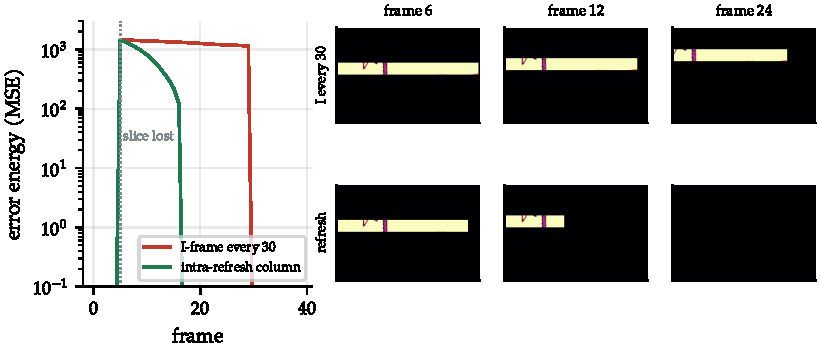
\includegraphics[width=0.92\linewidth]{figs/ch16_error_prop}\caption{An error that will not go away. A panning sequence loses one slice (16 rows)
in frame 5. Because every later frame is predicted from the damaged one, the error is copied forward,
moving with the picture, until something refreshes it. With an I-frame every 30 frames (red) it lasts
a full second; with an intra-refresh column sweeping across the picture (green) it is cleaned away
column by column within about 20 frames. Right: the error at frames 6, 12 and 24 for each scheme.}\label{fig:ch16_error_prop}\end{figure}

\subsection{Error resilience}

\mdcfig[0.85]{ch16_abr}{Adaptive streaming over a varying channel (a simulation with 4\,s segments, a
six-rung ladder from 0.4 to 7.5\,Mb/s and a 30\,s maximum buffer). Top: the available throughput and the
bit rate of the segments chosen by a player that streams at a fixed 3\,Mb/s and by an adaptive player that
uses the harmonic mean of recent throughput with a buffer-level safety rule. Bottom: the playback buffer.
During the deep fade between 150 and 205\,s the fixed-rate player drains its buffer and stalls; the adaptive
player drops to the lowest rungs, keeps playing, and climbs back when capacity returns.}

Because a video decoder predicts each frame from the previous ones, an error does not stay where it
lands: a corrupted block is copied into later frames by motion compensation, spreads spatially as vectors
point into it, and persists until the next intra refresh (Figure~\ref{fig:ch16_error_prop}). Codec
designers provide several layers of defence.

\begin{description}[style=nextline,leftmargin=1.2em,font=\sffamily\bfseries\small\color{navy}]
\item[Resynchronisation.] Frames are divided into \emph{slices}, each decodable independently of the
others in the same frame (entropy coding and intra prediction do not cross slice boundaries), and each
carried in its own packet. A lost packet costs one slice, not the frame.
\item[Limiting propagation.] Periodic I-frames or intra refresh bound how long an error persists;
\emph{reference picture selection} lets a decoder that reports a loss (through RTCP feedback in a video
call) ask the encoder to predict from an older, correctly received frame.
\item[Data partitioning and prioritisation.] Headers and motion vectors are much more important than
residual coefficients, so they can be separated and protected more strongly. H.264's data partitioning
and the NAL priority field support this.
\item[Concealment.] The decoder replaces lost blocks by interpolation from neighbours (spatial
concealment) or by copying from the previous frame with motion vectors estimated from neighbouring
blocks (temporal concealment). Good concealment hides most isolated slice losses.
\item[Forward error correction.] Below the codec, the transport adds FEC. Digital television in DVB-S,
DVB-T and DVB-C wraps the MPEG-2 transport stream's 188-byte packets in a Reed--Solomon RS(204,188) outer
code (Chapter~\ref{ch:classiccodes}), and DVB-S2 and DVB-T2 use BCH plus LDPC (Chapter~\ref{ch:moderncodes});
IPTV uses row--column XOR parity across packets (SMPTE 2022-1) or Raptor fountain codes; mobile broadcast
(3GPP MBMS) uses Raptor codes at the application layer so that receivers with different loss rates can all
recover.
\end{description}

\subsection{Adaptive bit-rate streaming}

For video on demand and live streaming over the internet, the dominant solution is not to protect a
single stream but to offer several. In \term{adaptive bit-rate streaming} (ABR) the content is encoded at
several rates and resolutions---a \emph{bit-rate ladder}---and each version is cut into segments of 2 to
10\,s, each starting with an I-frame so that the player can switch between versions at any segment
boundary. A \emph{manifest} file lists the versions and segment URLs. The player downloads segments over
ordinary HTTP (and hence through every cache and content-delivery network on the way), measures the
throughput it achieves, watches its playback buffer and chooses the version of the next segment. Apple's
\term{HTTP Live Streaming} (HLS, 2009, later RFC~8216) and the ISO standard \term{MPEG-DASH} (ISO/IEC
23009-1, 2012) are the two formats in use, now sharing a common segment format (CMAF). When your
film turns briefly soft as the train enters a tunnel and sharpens again afterwards, you are watching
the player step down and up its ladder.

The rate-selection algorithm (Figure~\ref{fig:ch16_abr}) is a control problem with conflicting goals:
maximise average quality, avoid stalls (rebuffering, which viewers hate far more than low quality) and
avoid frequent switching. \emph{Throughput-based} algorithms pick the highest rung below a conservative
estimate of recent throughput; \emph{buffer-based} algorithms (such as BBA, Huang et al., 2014) choose the
rate from the buffer level alone, on the principle that the buffer integrates the throughput history;
\emph{BOLA} (Spiteri et al., 2016) derives a buffer-based policy from Lyapunov optimisation and is the
default in the reference DASH player; model-predictive controllers optimise over a horizon of future
segments. Encoders also optimise the ladder itself: per-title and per-shot encoding choose the
resolution and rate of each rung from the content's own rate--quality curves, because a cartoon needs far
fewer bits than a football match. Low-latency variants (LL-HLS and low-latency DASH) cut segments into
sub-second chunks to bring live latency down to a few seconds.

ABR is joint source--channel coding at the system level: the source coder offers a menu of operating
points on its rate--distortion curve, and the transport chooses among them according to the channel
state---precisely the idea behind AMR's codec mode adaptation, at a thousand times the bit rate.


\begin{inpractice}[Video over the mobile network]
Video is the majority of mobile data traffic, and its behaviour shapes the network. ABR players respond to
the scheduler's allocation, which responds to the players' demand, and operators tune both: some cap
video resolution on congested cells, and most mobile video is delivered from caches inside or close to the
operator's network. For broadcast-like delivery of the same content to many users, LTE and 5G offer
multicast--broadcast services (eMBMS and 5G broadcast) with application-layer FEC. For real-time video
calls, where ABR's seconds of buffering are not available, the sender adapts instead: WebRTC's congestion
control estimates the available rate from packet delay and loss every few hundred milliseconds and
changes the encoder's target bit rate, resolution and frame rate on the fly, while temporal and spatial
scalability (SVC in VP9, AV1 and H.264 Annex~G) let a conferencing server forward different layers to
different participants without transcoding.
\end{inpractice}

%======================================================================

\begin{figure}[htbp]\centering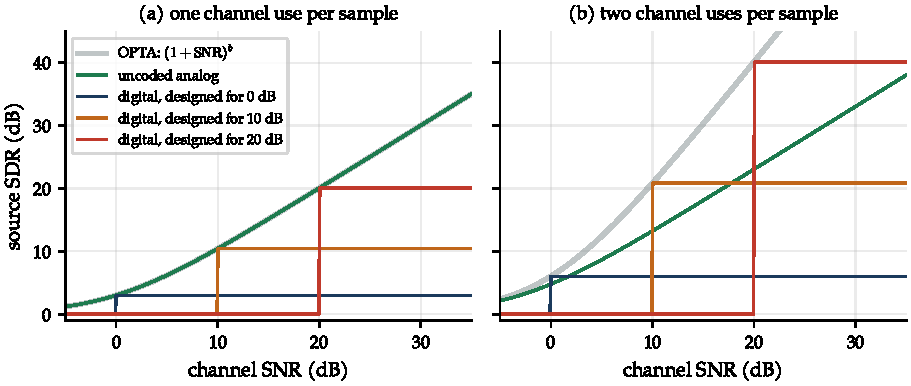
\includegraphics[width=0.92\linewidth]{figs/ch16_separation}\caption{Signal-to-distortion ratio of a Gaussian source sent over an AWGN channel.
(a) With one channel use per source sample, uncoded analogue transmission---scale the sample to the
power limit and send it; estimate it with a linear MMSE receiver---achieves the optimum $1+\mathrm{SNR}$
at \emph{every} SNR, while a separated digital system designed for a particular SNR reaches the optimum
only at its design point: it gains nothing above it and fails completely below it. (b) With two channel
uses per sample, the optimum rises to $(1+\mathrm{SNR})^2$, repeated analogue transmission achieves only
$1+2\,\mathrm{SNR}$, and digital coding designed for the right SNR wins by a wide margin.}\label{fig:ch16_separation}\end{figure}

\section{Joint source--channel coding}
\label{sec:ch16:jscc}
%======================================================================

\subsection{The separation theorem and its fine print}

Shannon's \term{source--channel separation theorem} (Chapter~\ref{ch:infotheory}) says that a source
with rate--distortion function $R(D)$ can be sent over a channel of capacity $C$ with distortion $D$ if
$R(D)<C$ (per unit time) and cannot if $R(D)>C$---and that the limit can be reached by designing the
source coder and the channel coder \emph{separately}, joined by a stream of equally likely bits. This is
the theorem that justifies the whole architecture of digital communication and the organisation of this
book: the source coder need not know about the channel, and the modem need not know whether its bits are
speech or spreadsheets.

For a Gaussian source of variance $\sigma^2$ sent over an AWGN channel with signal-to-noise ratio SNR,
using $b$ channel uses per source sample, setting $R(D)=bC$ gives the best achievable
\term{signal-to-distortion ratio}, often called the OPTA (optimum performance theoretically attainable):
\begin{equation}
\frac{\sigma^2}{D}=(1+\mathrm{SNR})^{\,b}.
\label{eq:ch16:opta}
\end{equation}

In words: every extra channel use per sample multiplies the achievable quality by another factor of
$(1+\mathrm{SNR})$. The theorem, however, has fine print, and every clause of it matters in practice.
\begin{description}[style=nextline,leftmargin=1.2em,font=\sffamily\bfseries\small\color{navy}]
\item[Unlimited delay and complexity.] Separation is optimal as block lengths go to infinity. At short
block lengths---a 20\,ms speech frame, a control message---both coders operate far from their limits, and
a joint design can do strictly better. Kostina and Verd\'u quantified the finite-blocklength penalty of
separation in 2013.
\item[A single, known channel.] The digital system is designed for a particular channel SNR. If the
actual SNR is higher, the extra quality is wasted, because the source was compressed for the design
rate; if lower, the channel code fails and the output collapses. This is the \term{cliff effect},
familiar to anyone who has watched digital television freeze while the analogue picture it replaced
would merely have become snowy (Figure~\ref{fig:ch16_separation}a).
\item[Point-to-point.] With several receivers of different quality (broadcasting), or several sources
(sensor networks, the multiple-access channel), separation is no longer optimal in general.
\end{description}


\begin{figure}[htbp]\centering
\begin{tikzpicture}[
  blk/.style={draw=navy,fill=navy!6,thick,rounded corners=2pt,minimum height=0.8cm,minimum width=1.5cm,align=center,font=\sffamily\scriptsize},
  arr/.style={-{Stealth[length=2mm]},thick}]
\node[blk] (enc) at (0,0) {scalable\\encoder};
\node[blk,fill=accent!10,draw=accent] (b) at (2.6,0.9) {base layer\\(robust: QPSK)};
\node[blk,fill=green!8,draw=green!50!black] (e) at (2.6,-0.9) {enhancement\\(fragile: 64-QAM)};
\draw[arr,navy] (enc)--(b); \draw[arr,navy] (enc)--(e);
\foreach \y/\snr/\got/\q in {1.6/{high SNR}/{base + enhancement}/{sharp HD},0/{medium SNR}/{base + part}/{good},-1.6/{low SNR}/{base only}/{soft but watchable}} {
  \node[blk,minimum width=2.6cm] (r) at (7.4,\y) {receiver at \snr\\decodes \got};
  \node[font=\sffamily\scriptsize,anchor=west,text=navy] at (8.85,\y) {$\Rightarrow$ \q};
  \draw[arr,navy!50] (3.9,0) -- (r.west);
}
\node[font=\sffamily\scriptsize,text=accent] at (5.0,-2.55) {no cliff: quality steps down gracefully};
\end{tikzpicture}
\caption{Layered coding with layered protection, the practical answer to the cliff effect of a single
digital design point. The base layer is coded and modulated so that every receiver gets it; each
enhancement layer reaches only the receivers whose channel is good enough. DVB-T hierarchical
modulation and scalable video (SVC, SHVC) work this way.}
\label{fig:ch16_layered}
\end{figure}

\subsection{When analogue is optimal}

The most striking counterexample is also the simplest. Take a memoryless Gaussian source and an AWGN
channel with one channel use per sample ($b=1$). Scale each sample to the transmit power, send it
\emph{uncoded}, and estimate it at the receiver with a linear minimum-mean-square-error estimator. The
resulting distortion is $\sigma^2/(1+\mathrm{SNR})$---exactly the OPTA~\eqref{eq:ch16:opta}, with no delay,
no complexity, no codebooks, and at every SNR simultaneously (Figure~\ref{fig:ch16_separation}a).
Thomas Goblick pointed this out in 1965, and Gastpar, Rimoldi and Vetterli characterised in 2003 exactly
when such ``uncoded'' transmission is optimal: when the source and channel are \emph{matched}, in the sense
that the channel's input cost and the source's distortion measure are the ones for which the channel's
optimal input and the source's optimal reconstruction coincide with the uncoded mapping. The match is
fragile. With two channel uses per sample (Figure~\ref{fig:ch16_separation}b) simple repetition gives
$1+2\,\mathrm{SNR}$, far below $(1+\mathrm{SNR})^2$ at high SNR, and digital coding wins; nonlinear
Shannon--Kotel'nikov mappings (spirals and other space-filling curves) that stretch one dimension into two
recover much of the gap while degrading gracefully.


The lesson is not that analogue beats digital; for sources with memory, perceptual distortion measures and
bandwidth mismatch, the digital approach wins overwhelmingly, and it allows compression, encryption,
multiplexing and regeneration that analogue signals do not. The lesson is that the graceful degradation of
analogue transmission is valuable, and that practical systems should try to recover some of it.

\subsection{Practical joint design}

Real systems retain the digital architecture but let the source and channel coders cooperate. The tools
appear throughout this chapter:
\begin{itemize}[nosep]
\item \emph{Unequal error protection}: protect the bits in proportion to their importance, as in the class
1a/1b/2 split of AMR in GSM and UMTS, the parity bit of G.729, and the prioritised NAL units of H.264.
\item \emph{Rate adaptation}: move the operating point along the rate--distortion curve as the channel
changes, as in AMR codec-mode adaptation, EVS channel-aware mode, WebRTC rate control and ABR streaming.
\item \emph{Layered (scalable) coding with layered transmission}: send a base layer robustly and
enhancement layers at higher rates, so that each receiver decodes as much as its channel allows (Figure~\ref{fig:ch16_layered}). DVB-T's
hierarchical modulation (a high-priority QPSK stream embedded in a 16- or 64-QAM constellation) and scalable
video (SVC, SHVC) are the classic examples; the broadcast channel of Chapter~\ref{ch:infotheory} explains
why superposition beats time-sharing.
\item \emph{Soft decoding using residual redundancy}: a source decoder that receives the channel decoder's
reliabilities, and uses the known structure and statistics of the source bits, can correct errors that the
channel code missed---for example, by choosing the most probable of the parameter values consistent with the
received soft bits. Iterative (turbo) source--channel decoding carries this further.
\item \emph{Channel-optimised quantisation}: design the quantiser's cells and the assignment of indices to
code vectors so that likely bit errors map to nearby reconstruction values (Farvardin and Vaishampayan,
1987--1991). The Gray-coded constellations of Chapter~\ref{ch:modulation} use the same idea for a different
purpose.
\item \emph{Analogue-like digital video}: SoftCast (Jakubczak and Katabi, 2011) sends scaled DCT coefficients
of video almost directly as the real and imaginary parts of OFDM symbols, so that quality degrades smoothly
with SNR in a multicast group, like the uncoded Gaussian system above.
\end{itemize}



\begin{figure}[htbp]\centering
\begin{tikzpicture}[
  net/.style={draw=navy,fill=navy!8,thick,trapezium,trapezium angle=70,minimum height=1.0cm,align=center,font=\sffamily\scriptsize,shape border rotate=270},
  netd/.style={net,shape border rotate=90},
  blk/.style={draw=navy,fill=navy!6,thick,rounded corners=2pt,minimum height=0.8cm,minimum width=1.2cm,align=center,font=\sffamily\scriptsize},
  arr/.style={-{Stealth[length=2mm]},thick,navy}]
\node[font=\sffamily\scriptsize,align=center] (x) at (0,0) {image\\$x$};
\node[net] (ga) at (1.9,0) {analysis\\net $g_a$};
\node[blk,draw=accent,fill=accent!8] (q) at (3.9,0) {quantise\\$\hat y$};
\node[blk] (ae) at (5.7,0) {arithmetic\\coder};
\node[blk] (ad) at (7.6,0) {arithmetic\\decoder};
\node[netd] (gs) at (9.6,0) {synthesis\\net $g_s$};
\node[font=\sffamily\scriptsize,align=center] (xh) at (11.4,0) {image\\$\hat x$};
\node[blk,fill=orange!8,draw=orange!70!black] (pm) at (6.65,1.5) {learned probability\\model (hyperprior)};
\draw[arr] (x)--(ga); \draw[arr] (ga)--node[above,font=\tiny]{latents $y$}(q); \draw[arr] (q)--(ae);
\draw[arr] (ae)--node[above,font=\tiny]{bits}(ad); \draw[arr] (ad)--(gs); \draw[arr] (gs)--(xh);
\draw[arr,orange!70!black] (pm)--(ae); \draw[arr,orange!70!black] (pm)--(ad);
\node[font=\sffamily\scriptsize,text=accent,align=center] at (5.7,-1.25) {trained end to end to minimise $D(x,\hat x)+\lambda R$};
\end{tikzpicture}
\caption{A learned image codec. The same three stages as Figure~\ref{fig:ch16_chain}---transform,
quantise, entropy code---but the transform and its inverse are neural networks and the probability
model that drives the arithmetic coder is learned too, all trained together on a rate--distortion
objective.}
\label{fig:ch16_learned}
\end{figure}

\begin{keyidea}[Separation is a design principle, not a law of nature]
Separate source and channel coding is optimal in the limit of infinite delay for a single known channel,
and it is the right default because it makes systems modular. But real links have finite delay, varying
channels and many receivers. The best systems keep the digital interface and add cross-layer hooks: bit
priorities, rate adaptation, scalable layers and soft information passed up the stack. Whenever a design
review hears ``the codec doesn't need to know about the channel,'' someone should ask about the cliff.
\end{keyidea}

%======================================================================

\section{Learned codecs}
\label{sec:ch16:neural}
%======================================================================


Every codec in this chapter was designed by hand: engineers chose the transform, the quantiser, the
contexts and the perceptual model and tuned them on test material. Since about 2016, neural networks have
been used to learn all of these components end to end (Figure~\ref{fig:ch16_learned}). A learned image
codec (Ball\'e, Laparra and Simoncelli, 2017) replaces the DCT with a convolutional \emph{analysis}
network that maps the image to a latent representation, quantises the latents uniformly, entropy codes
them with an arithmetic coder driven by a learned probability model, and reconstructs with a
\emph{synthesis} network. The whole system is trained to minimise $D+\lambda R$, the Lagrangian of
Section~\ref{sec:ch16:video}, with the rate estimated differentiably from the learned probability model.

Adding a \emph{hyperprior}---a small side channel that describes the local scale of the latents so that
the entropy model can adapt (Ball\'e et al., 2018)---made learned codecs competitive with the best
conventional intra coders in PSNR, and they surpass them on perceptual metrics, especially at low rates.
The JPEG committee's JPEG~AI project (ISO/IEC~6048) is the first international standard for a learned
image codec.


In audio, neural codecs such as Google's SoundStream (2021, used in the Lyra v2 codec) and Meta's EnCodec
(2022) use a convolutional encoder, a \emph{residual vector quantiser}---a cascade of small VQ stages, each
quantising the error of the previous one, the multistage VQ of Section~\ref{sec:ch16:lossy} reborn---and a
decoder trained with adversarial and perceptual losses. Figure~\ref{fig:ch16_rvq} shows the quantiser's structure. They code speech at 3--6\,kb/s with quality that, in their
authors' listening tests, conventional codecs needed several times the rate to match, and their discrete codes have become the
``tokens'' with which audio language models listen and speak. Generative decoders go further still: at very
low rates they do not reproduce the signal so much as synthesise a plausible signal consistent with the
transmitted description, which blurs the line between a codec and a generative model.

The obstacles to deployment are practical rather than theoretical: decoder complexity and power on phones,
the need for bit-exact, platform-independent decoding in a standard, and the difficulty of guaranteeing
behaviour on content unlike the training data. The same ideas, extended to include the channel, appear as
\emph{deep joint source--channel coding} (Bourtsoulatze, Kurka and G\"und\"uz, 2019), in which a network maps
images directly to channel symbols and degrades gracefully with SNR, and as the ``semantic communication''
studied for 6G, taken up in Chapter~\ref{ch:sixg}.

\begin{figure}[htbp]\centering
\begin{tikzpicture}[
  blk/.style={draw=navy,fill=navy!6,thick,rounded corners=2pt,minimum height=0.75cm,minimum width=1.35cm,align=center,font=\sffamily\scriptsize},
  q/.style={blk,draw=accent,fill=accent!8},
  sm/.style={draw=navy,circle,thick,minimum size=0.45cm,inner sep=0pt,font=\sffamily\small},
  arr/.style={-{Stealth[length=2mm]},thick,navy}]
\node[font=\sffamily\scriptsize,align=center] (x) at (0,0) {latent\\vector};
\node[q] (q1) at (1.9,0) {VQ stage 1\\(1024 entries)};
\node[sm] (s1) at (1.9,-1.3) {$-$};
\node[q] (q2) at (4.3,-1.3) {VQ stage 2};
\node[sm] (s2) at (4.3,-2.6) {$-$};
\node[q] (q3) at (6.7,-2.6) {VQ stage 3};
\node[font=\sffamily\scriptsize] (dots) at (8.6,-2.6) {$\cdots$};
\node[blk,fill=green!6,draw=green!50!black] (out) at (9.6,0) {indices\\$i_1,i_2,i_3,\dots$};
\draw[arr] (x)--(q1); \draw[arr] (x) |- (s1);
\draw[arr] (q1)--(s1);
\draw[arr] (s1)--node[above,font=\tiny]{residual}(q2); \draw[arr] (s1) |- (s2); \draw[arr] (q2)--(s2);
\draw[arr] (s2)--node[above,font=\tiny]{residual}(q3); \draw[arr] (q3)--(dots);
\draw[arr,green!50!black] (q1)--(out); \draw[arr,green!50!black] (q2) |- ([yshift=-4pt]out.west);
\draw[arr,green!50!black] (q3) |- ([yshift=-9pt]out.south west);
\end{tikzpicture}
\caption{The residual vector quantiser of neural audio codecs such as SoundStream and EnCodec. Each
stage quantises what the previous stages missed, so a few small codebooks act like one enormous one;
dropping the last stages lowers the bit rate gracefully, which is how one trained model serves several
rates.}
\label{fig:ch16_rvq}
\end{figure}

\begin{pitfall}[A codec that invents plausible content]
A codec that fills in detail from a learned model can produce output that looks right and is wrong. The
risk is not hypothetical. In 2013 the computer scientist David Kriesel found that certain Xerox scanners,
compressing documents with the JBIG2 standard's pattern-matching mode, replaced some digits with other
digits that looked similar---a 6 in a building plan became an 8---because symbols judged similar were coded
as copies of a single stored pattern. The scans looked perfectly crisp. For medical images, legal documents,
text, numbers and anything used as evidence, a codec must not substitute plausible content for actual
content, and learned codecs must be evaluated for exactly this failure.
\end{pitfall}

%======================================================================
\section{Summary}
%======================================================================

\begin{itemize}
\item Compression removes redundancy (reversibly, bounded by entropy; Figure~\ref{fig:ch16_summary_ratios} sums up the ratios) and irrelevance (irreversibly,
bounded by the rate--distortion function under a perceptual distortion measure). It is the cheapest way to
buy capacity, and it produced the factors of 10 to 500 of Table~\ref{tab:ch16:rates}.
\item Huffman codes are optimal symbol codes but lose up to a bit per symbol; arithmetic coding, range
coding and ANS reach the ideal adaptive code length and separate modelling from coding. CABAC is the
context-adaptive binary arithmetic coder of modern video. Golomb--Rice and exp-Golomb codes suit geometric
sources; Lempel--Ziv coders (DEFLATE, LZMA, Zstandard) are universal and dominate general-purpose data.
\item Entropy-coded uniform quantisation is within 1.53\,dB (0.254\,bit) of the rate--distortion bound at high
rate; vector quantisation closes the gap only slowly but exploits memory. Transforms concentrate energy;
the coding gain is the ratio of arithmetic to geometric mean of the coefficient variances; the DCT is nearly
the KLT for correlated sources; reverse water-filling explains why small coefficients are discarded.
\item Speech codecs model the source--filter production mechanism with linear prediction (Levinson--Durbin,
reflection coefficients, LSFs). CELP's analysis-by-synthesis search with adaptive and algebraic codebooks
and perceptual weighting underlies G.729, AMR, AMR-WB and EVS; Opus merges LPC and MDCT coding for the
internet. Quality is measured by MOS, PESQ and POLQA. The ``phone-y'' sound is the 3.4\,kHz band, not
the codec.

\item Audio codecs model the listener: the threshold in quiet, critical bands and simultaneous and temporal
masking. The MDCT with TDAC gives critically sampled, overlapped filterbanks; block switching and TNS control
pre-echo; MP3 and AAC add bit reservoirs and joint stereo; SBR and parametric stereo synthesise what is not
sent. A 128\,kb/s MP3 sounds clean because its noise is shaped to hide under the music.
\item Image codecs use colour transforms and chroma subsampling, then transform coding: JPEG's $8\times8$ DCT,
quantisation tables, zigzag and run-length Huffman coding; JPEG~2000's wavelets and embedded bit-plane
coding; and the intra modes of video codecs in WebP, HEIC and AVIF. Smooth dark gradients are where block
codecs fail first.
\begin{figure}[H]\centering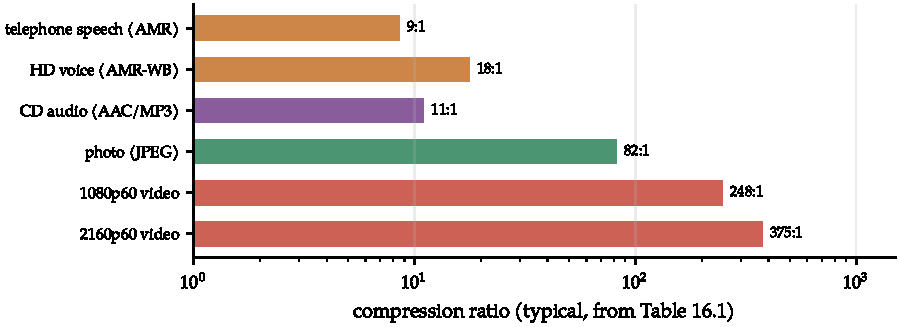
\includegraphics[width=0.92\linewidth]{figs/ch16_summary_ratios}\caption{The chapter in one picture: typical compression ratios of the codecs
of Table~\ref{tab:ch16:rates}, on a logarithmic scale. Speech gains a factor of ten from modelling the
talker, audio a factor of ten from modelling the listener, and video a factor of several hundred
from modelling both the viewer and the motion.}\label{fig:ch16_summary_ratios}\end{figure}

\item Video codecs are hybrid: motion-compensated prediction with a decoder in the loop, transform coding of
the residual, rate--distortion optimised decisions and rate control. Each generation from H.261 to VVC and AV1
has roughly halved the bit rate.
\item Compressed streams are fragile and variable in rate. Slices, intra refresh, concealment, FEC and
adaptive streaming match them to real channels. Separation is optimal only asymptotically; unequal
protection, rate adaptation and layered coding recover the graceful degradation that analogue systems had
for free. Learned codecs are the newest chapter in the story.
\end{itemize}

\begin{labbox}[Source coding, live]
Lab 24, \lab{moderncomms-labs/labs/lab24\_source\_coding.py} (run it with
\lab{python lab24\_source\_coding.py}), turns this chapter into nine interactive experiments:
\begin{itemize}
\item \textbf{Huffman vs arithmetic coding}: type any text (or load the book text) and compare the
Huffman code lengths and an adaptive order-0 to order-3 arithmetic coder with the entropy and with zlib,
bzip2 and xz (Figures~\ref{fig:ch16_huffman} and~\ref{fig:ch16_huff_redundancy}).
\item \textbf{LZ77: the sliding window}: step through a parse token by token and see the effect of the
window size and maximum match length (Figures~\ref{fig:ch16_lz77_parse} and~\ref{fig:ch16_compress_speed}).
\item \textbf{Quantisers and Lloyd--Max}: run Lloyd's algorithm one iteration at a time on Gaussian,
Laplacian and uniform sources (Figures~\ref{fig:ch16_lloyd_iter} and~\ref{fig:ch16_quantizers}).
\item \textbf{DCT energy compaction}: pick any $8\times8$ block, keep the first $k$ coefficients and watch
the rebuild (Figures~\ref{fig:ch16_dct_recipe} and~\ref{fig:ch16_compaction}).
\item \textbf{A toy JPEG}: the complete baseline pipeline with a quality slider, bit rate, PSNR and error
view (Figures~\ref{fig:ch16_jpeg_block}, \ref{fig:ch16_jpeg_quality} and~\ref{fig:ch16_jpeg_zoom}).
\item \textbf{LPC: a buzz and a filter}: analyse three vowels, change the predictor order, and resynthesise
at a new pitch or as a whisper---and listen (Figures~\ref{fig:ch16_vowel_lpc} and~\ref{fig:ch16_source_filter}).
\item \textbf{Masking: hide a tone} and \textbf{Noise under the mask}: move a masker and a probe, and hear
shaped and white noise of equal power (Figures~\ref{fig:ch16_masking} and~\ref{fig:ch16_noise_shaping}).
\item \textbf{Motion estimation}: set a camera pan and a moving ball, then vary the block size and search
range (Figure~\ref{fig:ch16_motion}).
\end{itemize}
The figure script \lab{book/figscripts/ch16\_figs.py} generates every data figure in this chapter,
including the rate--distortion comparison with real codecs, and is a good starting point for further
experiments.
\end{labbox}

\problems
\begin{enumerate}[label=\thechapter.\arabic*]
\item A source emits symbols with probabilities 0.4, 0.2, 0.15, 0.1, 0.1, 0.05. Construct a Huffman code,
compute its average length and efficiency, and write down the corresponding canonical code. Is the Huffman
code unique? Are its codeword lengths unique?
\item A binary source has $P(1)=0.05$. (a) What is its entropy? (b) What average length does a Huffman code
achieve on single symbols, on pairs and on triples? (c) Design a Golomb code for the run lengths of zeros
between ones and compare its rate with the entropy.
\item Encode the message \texttt{bcab} with the arithmetic coder of Figure~\ref{fig:ch16_arithmetic}. Find the
final interval and the shortest binary fraction inside it. Then decode your fraction, assuming the decoder
knows the message has four symbols.
\item Parse the string \texttt{abababababbbbbb} with LZ77 (unbounded window, minimum match length 2) and with
LZW starting from the dictionary $\{a,b\}$. Count the output symbols in each case.
\item Show that for a uniform quantiser with step $\Delta$ and a smooth density, the output entropy is
approximately $h(X)-\log_2\Delta$. Use it to derive~\eqref{eq:ch16:ecsq}, and compute the gap to the
rate--distortion bound for a Laplacian source (whose $R(D)$ at high rate is given by the Shannon lower bound).
\item Compute the coding gain of the KLT and of the DCT for an AR(1) source with $\rho=0.9$ and $N=4$. Using
reverse water-filling, find the bit allocation for an average of 1 bit per sample and the resulting SNR.
\item A speech frame has normalised autocorrelation $r=[1,\,0.9,\,0.7,\,0.45]$. Run the Levinson--Durbin
recursion to order 3. Give the reflection coefficients, the predictor, the prediction gain after each order,
and check that the synthesis filter is stable.
\item For the order-2 predictor of the worked example in Section~\ref{sec:ch16:lpc}, form $P(z)$ and $Q(z)$,
find their roots and verify that the LSFs interleave. What happens to the LSFs as the pole radius
approaches one?
\item G.729 sends 80 bits per 10\,ms frame. How many bits per second go to the spectral envelope, the pitch,
the fixed codebook and the gains? If the codec were carried in RTP/UDP/IPv4 packets with two frames per packet,
what would the IP-layer bit rate be, and what fraction is header?
\item A tone at 1\,kHz and 70\,dB SPL is present. Using~\eqref{eq:ch16:bark} and the spreading function and
offsets of Figure~\ref{fig:ch16_masking}, estimate the maximum level of an inaudible noise band at 1.5\,kHz
and at 700\,Hz. Explain the asymmetry.
\item Show that the sine window satisfies the Princen--Bradley condition~\eqref{eq:ch16:pb}. For an MDCT with
$N=1024$ at 48\,kHz, what are the frequency resolution and the time span over which pre-echo can spread? Repeat
for AAC's short blocks.
\item An image is coded with JPEG at 0.8 bits per pixel. Estimate the size of a $4000\times3000$ photograph
(luma and 4:2:0 chroma, with chroma costing about a quarter of the luma bits). What compression ratio is this
relative to 24-bit RGB?
\item A 4K (3840$\times$2160) 60 frame/s 10-bit 4:2:0 stream is coded with HEVC at 16\,Mb/s. Compute the raw rate,
the compression ratio and the bits per pixel. Using the frame-size model of the worked example (I $=8P$,
B $=P/2$, GOP of 64 frames with 3 B-frames between references), find the size of an I-frame.
\item \emph{(Simulation)} Implement an adaptive order-$k$ arithmetic coder model (count-based, with the
estimator of Figure~\ref{fig:ch16_huffman}) and measure the code length on a long English text for $k=0$ to 5.
Plot bits per character against $k$ and against text length, and explain the context-dilution effect.
\item \emph{(Simulation)} Extend the chapter's toy JPEG with (a) a deadzone quantiser and (b) trellis-free
``RD-optimised'' zeroing of isolated $\pm1$ coefficients whose removal saves more than $\lambda$ times the
distortion increase. Plot the rate--PSNR curves against the baseline and against libjpeg.
\item \emph{(Simulation)} Simulate a Gaussian source over an AWGN channel with (a) uncoded linear transmission
and (b) a scalar quantiser with 8 levels, Gray-mapped onto 8-PAM. Plot the SDR against channel SNR from 0 to
30\,dB, and compare both with the OPTA. Where does each scheme win?
\item \emph{(Simulation)} Reproduce Figure~\ref{fig:ch16_dark_scene}: code a smooth gradient whose
values span 18--32 with JPEG at quality 25 and measure the PSNR and the largest step between adjacent
blocks. Then add Gaussian noise of standard deviation 1 before coding (dither). Does the PSNR improve
or worsen? Does the picture? Relate your answer to the film-grain synthesis of
Figure~\ref{fig:ch16_film_grain}.
\item In Lab~24's \emph{Noise under the mask}, the SNR readout stays the same when you switch between
shaped and white noise. Using Figure~\ref{fig:ch16_noise_shaping}, explain why, and estimate how many
bits per sample a PCM coder would need to make white noise inaudible over the whole band if the
lowest point of the masking threshold lies 60\,dB below the loudest spectral line.
\end{enumerate}

\furtherreading
\begin{itemize}
\item K.~Sayood, \emph{Introduction to Data Compression}, 5th ed., Morgan Kaufmann, 2017. A readable, broad
textbook covering lossless coding, quantisation, transforms and the main media standards.
\item A.~Gersho and R.~M.~Gray, \emph{Vector Quantization and Signal Compression}, Kluwer, 1992. The
definitive treatment of scalar and vector quantisation, predictive and transform coding and bit allocation.
\item N.~S.~Jayant and P.~Noll, \emph{Digital Coding of Waveforms}, Prentice Hall, 1984. The classic on PCM,
DPCM, ADPCM, transform and subband coding of speech and images, with the coding-gain analysis of this chapter.
\item I.~H.~Witten, R.~M.~Neal and J.~G.~Cleary, ``Arithmetic coding for data compression,''
\emph{Communications of the ACM}, vol.~30, no.~6, 1987. The paper that made arithmetic coding practical, with
working code.
\item L.~R.~Rabiner and R.~W.~Schafer, \emph{Theory and Applications of Digital Speech Processing}, Pearson,
2011. Speech production, linear prediction and speech coding from the pioneers of the field.
\item A.~M.~Kondoz, \emph{Digital Speech: Coding for Low Bit Rate Communication Systems}, 2nd ed., Wiley,
2004. Detailed descriptions of CELP and its standardised variants.
\item T.~Painter and A.~Spanias, ``Perceptual coding of digital audio,'' \emph{Proceedings of the IEEE},
vol.~88, no.~4, 2000. An excellent tutorial survey of psychoacoustics, filterbanks and the MPEG and Dolby
coders.
\item G.~K.~Wallace, ``The JPEG still picture compression standard,'' \emph{Communications of the ACM},
vol.~34, no.~4, 1991. A clear overview by the chair of the JPEG committee.
\item D.~S.~Taubman and M.~W.~Marcellin, \emph{JPEG2000: Image Compression Fundamentals, Standards and
Practice}, Kluwer, 2002. Wavelets, embedded coding and EBCOT from the inventor of EBCOT.
\item T.~Wiegand, G.~J.~Sullivan, G.~Bj{\o}ntegaard and A.~Luthra, ``Overview of the H.264/AVC video coding
standard,'' \emph{IEEE Transactions on Circuits and Systems for Video Technology}, vol.~13, no.~7, 2003; with
the companion overviews of HEVC (Sullivan et al., same journal, vol.~22, no.~12, 2012) and VVC (Bross et al.,
vol.~31, no.~10, 2021). The authoritative introductions to each standard.
\item M.~Gastpar, B.~Rimoldi and M.~Vetterli, ``To code, or not to code: lossy source--channel communication
revisited,'' \emph{IEEE Transactions on Information Theory}, vol.~49, no.~5, 2003. When uncoded transmission is
optimal, and why.
\item J.~Ball\'e, V.~Laparra and E.~P.~Simoncelli, ``End-to-end optimized image compression,''
\emph{International Conference on Learning Representations} (ICLR), 2017. The paper that launched learned image
compression.
\end{itemize}
